\documentclass[11pt]{article}

% The four macros of the header standard; tools/zenodo/publish_revision.py patches them when it reserves the DOI.
\newcommand{\doctype}{Preprint}
\newcommand{\docversion}{v1.00.000}
\newcommand{\docdate}{6 November 2026}
\newcommand{\versiondoi}{10.5281/zenodo.0}
\newcommand{\conceptdoi}{10.5281/zenodo.0}
\newcommand{\docidentity}{CAOS\_Contraste, the validation of the risk models of a bank}

% The packages and conventions every Contraste manuscript shares (CAOS_MANAGE conventions/manuscript-content-bar.md
% section 2). A document sets its class, the four header macros and \docidentity, then % The packages and conventions every Contraste manuscript shares (CAOS_MANAGE conventions/manuscript-content-bar.md
% section 2). A document sets its class, the four header macros and \docidentity, then % The packages and conventions every Contraste manuscript shares (CAOS_MANAGE conventions/manuscript-content-bar.md
% section 2). A document sets its class, the four header macros and \docidentity, then \input{../_shared/preamble}.
\usepackage[T1]{fontenc}
\usepackage[utf8]{inputenc}
\usepackage{lmodern}
\usepackage{microtype}
\usepackage[a4paper,margin=2.5cm]{geometry}
\usepackage{amsmath,amssymb,amsthm,mathtools,bm}
\usepackage{graphicx}
\usepackage{booktabs,longtable,tabularx,array,multirow}
\usepackage{siunitx}
\usepackage{algorithm}
\usepackage{algpseudocode}
\usepackage{caption,subcaption}
\usepackage{xcolor}
\usepackage[numbers,sort&compress]{natbib}
\usepackage[hidelinks]{hyperref}
\usepackage{cleveref}
\usepackage{orcidlink}

\sisetup{group-separator={,},group-minimum-digits=4,detect-all}
\graphicspath{{figures/}{../figures/}}
\captionsetup{font=small,labelfont=bf}
\setlength{\LTcapwidth}{\textwidth}

% Theorem environments for the Theory sections of the manuscripts.
\newtheorem{proposition}{Proposition}
\newtheorem{lemma}{Lemma}
\newtheorem{corollary}{Corollary}
\theoremstyle{definition}
\newtheorem{definition}{Definition}
\newtheorem{assumption}{Assumption}
\theoremstyle{remark}
\newtheorem{remark}{Remark}

% Notation shared by the documents (each defines it again in its notation table).
\newcommand{\E}{\mathbb{E}}
\newcommand{\Prob}{\mathbb{P}}
\newcommand{\Var}{\operatorname{Var}}
\newcommand{\Cov}{\operatorname{Cov}}
\newcommand{\VaR}{\operatorname{VaR}}
\newcommand{\ES}{\operatorname{ES}}
\newcommand{\PD}{\mathrm{PD}}
\newcommand{\LGD}{\mathrm{LGD}}
\newcommand{\EAD}{\mathrm{EAD}}
\newcommand{\ECL}{\mathrm{ECL}}
\newcommand{\indic}{\mathbf{1}}
\newcommand{\R}{\mathbb{R}}
\newcommand{\dd}{\,\mathrm{d}}

% The page-1 header block (CAOS_MANAGE conventions/manuscript-header-standard.md). The document defines \doctype,
% \docversion, \docdate, \versiondoi, \conceptdoi and \docidentity before this file; the publishing tool patches the four
% macros of the standard when it reserves the version DOI.
\newcommand{\docrepo}{github.com/fsantibanezleal/CAOS\_Contraste}
\newcommand{\headerblock}{%
\begin{center}
\fbox{\parbox{0.94\textwidth}{\small\raggedright
\textbf{\doctype} \quad$\cdot$\quad \docversion, \docdate \quad$\cdot$\quad Licence CC BY 4.0\\[2pt]
CAOS open-research programme \quad$\cdot$\quad \docidentity\\[2pt]
Version DOI \href{https://doi.org/\versiondoi}{\texttt{\versiondoi}} \quad$\cdot$\quad
concept DOI (always latest) \href{https://doi.org/\conceptdoi}{\texttt{\conceptdoi}}\\[2pt]
Not peer reviewed. Source code, data and computational records: \href{https://\docrepo}{\texttt{\docrepo}}
}}
\end{center}
\vspace{4pt}}
.
\usepackage[T1]{fontenc}
\usepackage[utf8]{inputenc}
\usepackage{lmodern}
\usepackage{microtype}
\usepackage[a4paper,margin=2.5cm]{geometry}
\usepackage{amsmath,amssymb,amsthm,mathtools,bm}
\usepackage{graphicx}
\usepackage{booktabs,longtable,tabularx,array,multirow}
\usepackage{siunitx}
\usepackage{algorithm}
\usepackage{algpseudocode}
\usepackage{caption,subcaption}
\usepackage{xcolor}
\usepackage[numbers,sort&compress]{natbib}
\usepackage[hidelinks]{hyperref}
\usepackage{cleveref}
\usepackage{orcidlink}

\sisetup{group-separator={,},group-minimum-digits=4,detect-all}
\graphicspath{{figures/}{../figures/}}
\captionsetup{font=small,labelfont=bf}
\setlength{\LTcapwidth}{\textwidth}

% Theorem environments for the Theory sections of the manuscripts.
\newtheorem{proposition}{Proposition}
\newtheorem{lemma}{Lemma}
\newtheorem{corollary}{Corollary}
\theoremstyle{definition}
\newtheorem{definition}{Definition}
\newtheorem{assumption}{Assumption}
\theoremstyle{remark}
\newtheorem{remark}{Remark}

% Notation shared by the documents (each defines it again in its notation table).
\newcommand{\E}{\mathbb{E}}
\newcommand{\Prob}{\mathbb{P}}
\newcommand{\Var}{\operatorname{Var}}
\newcommand{\Cov}{\operatorname{Cov}}
\newcommand{\VaR}{\operatorname{VaR}}
\newcommand{\ES}{\operatorname{ES}}
\newcommand{\PD}{\mathrm{PD}}
\newcommand{\LGD}{\mathrm{LGD}}
\newcommand{\EAD}{\mathrm{EAD}}
\newcommand{\ECL}{\mathrm{ECL}}
\newcommand{\indic}{\mathbf{1}}
\newcommand{\R}{\mathbb{R}}
\newcommand{\dd}{\,\mathrm{d}}

% The page-1 header block (CAOS_MANAGE conventions/manuscript-header-standard.md). The document defines \doctype,
% \docversion, \docdate, \versiondoi, \conceptdoi and \docidentity before this file; the publishing tool patches the four
% macros of the standard when it reserves the version DOI.
\newcommand{\docrepo}{github.com/fsantibanezleal/CAOS\_Contraste}
\newcommand{\headerblock}{%
\begin{center}
\fbox{\parbox{0.94\textwidth}{\small\raggedright
\textbf{\doctype} \quad$\cdot$\quad \docversion, \docdate \quad$\cdot$\quad Licence CC BY 4.0\\[2pt]
CAOS open-research programme \quad$\cdot$\quad \docidentity\\[2pt]
Version DOI \href{https://doi.org/\versiondoi}{\texttt{\versiondoi}} \quad$\cdot$\quad
concept DOI (always latest) \href{https://doi.org/\conceptdoi}{\texttt{\conceptdoi}}\\[2pt]
Not peer reviewed. Source code, data and computational records: \href{https://\docrepo}{\texttt{\docrepo}}
}}
\end{center}
\vspace{4pt}}
.
\usepackage[T1]{fontenc}
\usepackage[utf8]{inputenc}
\usepackage{lmodern}
\usepackage{microtype}
\usepackage[a4paper,margin=2.5cm]{geometry}
\usepackage{amsmath,amssymb,amsthm,mathtools,bm}
\usepackage{graphicx}
\usepackage{booktabs,longtable,tabularx,array,multirow}
\usepackage{siunitx}
\usepackage{algorithm}
\usepackage{algpseudocode}
\usepackage{caption,subcaption}
\usepackage{xcolor}
\usepackage[numbers,sort&compress]{natbib}
\usepackage[hidelinks]{hyperref}
\usepackage{cleveref}
\usepackage{orcidlink}

\sisetup{group-separator={,},group-minimum-digits=4,detect-all}
\graphicspath{{figures/}{../figures/}}
\captionsetup{font=small,labelfont=bf}
\setlength{\LTcapwidth}{\textwidth}

% Theorem environments for the Theory sections of the manuscripts.
\newtheorem{proposition}{Proposition}
\newtheorem{lemma}{Lemma}
\newtheorem{corollary}{Corollary}
\theoremstyle{definition}
\newtheorem{definition}{Definition}
\newtheorem{assumption}{Assumption}
\theoremstyle{remark}
\newtheorem{remark}{Remark}

% Notation shared by the documents (each defines it again in its notation table).
\newcommand{\E}{\mathbb{E}}
\newcommand{\Prob}{\mathbb{P}}
\newcommand{\Var}{\operatorname{Var}}
\newcommand{\Cov}{\operatorname{Cov}}
\newcommand{\VaR}{\operatorname{VaR}}
\newcommand{\ES}{\operatorname{ES}}
\newcommand{\PD}{\mathrm{PD}}
\newcommand{\LGD}{\mathrm{LGD}}
\newcommand{\EAD}{\mathrm{EAD}}
\newcommand{\ECL}{\mathrm{ECL}}
\newcommand{\indic}{\mathbf{1}}
\newcommand{\R}{\mathbb{R}}
\newcommand{\dd}{\,\mathrm{d}}

% The page-1 header block (CAOS_MANAGE conventions/manuscript-header-standard.md). The document defines \doctype,
% \docversion, \docdate, \versiondoi, \conceptdoi and \docidentity before this file; the publishing tool patches the four
% macros of the standard when it reserves the version DOI.
\newcommand{\docrepo}{github.com/fsantibanezleal/CAOS\_Contraste}
\newcommand{\headerblock}{%
\begin{center}
\fbox{\parbox{0.94\textwidth}{\small\raggedright
\textbf{\doctype} \quad$\cdot$\quad \docversion, \docdate \quad$\cdot$\quad Licence CC BY 4.0\\[2pt]
CAOS open-research programme \quad$\cdot$\quad \docidentity\\[2pt]
Version DOI \href{https://doi.org/\versiondoi}{\texttt{\versiondoi}} \quad$\cdot$\quad
concept DOI (always latest) \href{https://doi.org/\conceptdoi}{\texttt{\conceptdoi}}\\[2pt]
Not peer reviewed. Source code, data and computational records: \href{https://\docrepo}{\texttt{\docrepo}}
}}
\end{center}
\vspace{4pt}}

% The number macros written by tables/make_tables.py from experiments/results.json (definitions only, no conditional).
% Written by tables/make_tables.py from experiments/results.json: one macro per number quoted in the text.
\newcommand{\abClosedformCells}{16}
\newcommand{\abClosedformDelta}{25.4}
\newcommand{\abClosedformFrom}{34.0}
\newcommand{\abClosedformHi}{26.6}
\newcommand{\abClosedformLo}{24.3}
\newcommand{\abClosedformN}{10{,}743}
\newcommand{\abClosedformTo}{59.5}
\newcommand{\abCvmCells}{16}
\newcommand{\abCvmDelta}{-14.6}
\newcommand{\abCvmDown}{14.6}
\newcommand{\abCvmDownHi}{15.7}
\newcommand{\abCvmDownLo}{13.5}
\newcommand{\abCvmFrom}{62.2}
\newcommand{\abCvmHi}{-13.5}
\newcommand{\abCvmLo}{-15.7}
\newcommand{\abCvmN}{10{,}371}
\newcommand{\abCvmTo}{47.6}
\newcommand{\abExpertpriorCells}{16}
\newcommand{\abExpertpriorDelta}{48.5}
\newcommand{\abExpertpriorFrom}{34.0}
\newcommand{\abExpertpriorHi}{49.6}
\newcommand{\abExpertpriorLo}{47.3}
\newcommand{\abExpertpriorN}{10{,}743}
\newcommand{\abExpertpriorTo}{82.5}
\newcommand{\abHeavytailCells}{15}
\newcommand{\abHeavytailDelta}{21.6}
\newcommand{\abHeavytailFrom}{13.6}
\newcommand{\abHeavytailHi}{22.9}
\newcommand{\abHeavytailLo}{20.4}
\newcommand{\abHeavytailN}{9{,}385}
\newcommand{\abHeavytailTo}{35.2}
\newcommand{\abMeanadjustedCells}{16}
\newcommand{\abMeanadjustedDelta}{3.0}
\newcommand{\abMeanadjustedFrom}{58.6}
\newcommand{\abMeanadjustedHi}{3.4}
\newcommand{\abMeanadjustedLo}{2.6}
\newcommand{\abMeanadjustedN}{11{,}337}
\newcommand{\abMeanadjustedTo}{61.6}
\newcommand{\abMeancorrectionCells}{12}
\newcommand{\abMeancorrectionDelta}{2.9}
\newcommand{\abMeancorrectionFrom}{62.5}
\newcommand{\abMeancorrectionHi}{3.4}
\newcommand{\abMeancorrectionLo}{2.5}
\newcommand{\abMeancorrectionN}{10{,}635}
\newcommand{\abMeancorrectionTo}{65.5}
\newcommand{\abObreCells}{16}
\newcommand{\abObreDelta}{-1.7}
\newcommand{\abObreDown}{1.7}
\newcommand{\abObreDownHi}{2.4}
\newcommand{\abObreDownLo}{1.0}
\newcommand{\abObreFrom}{61.7}
\newcommand{\abObreHi}{-1.0}
\newcommand{\abObreLo}{-2.4}
\newcommand{\abObreN}{10{,}941}
\newcommand{\abObreTo}{60.0}
\newcommand{\abThresholdCells}{16}
\newcommand{\abThresholdDelta}{14.8}
\newcommand{\abThresholdFrom}{0.0}
\newcommand{\abThresholdHi}{15.5}
\newcommand{\abThresholdLo}{14.2}
\newcommand{\abThresholdN}{11{,}876}
\newcommand{\abThresholdTo}{14.8}
\newcommand{\abWrongfamilyCells}{15}
\newcommand{\abWrongfamilyDelta}{-44.2}
\newcommand{\abWrongfamilyFrom}{49.1}
\newcommand{\abWrongfamilyHi}{-43.1}
\newcommand{\abWrongfamilyLo}{-45.3}
\newcommand{\abWrongfamilyN}{10{,}275}
\newcommand{\abWrongfamilyTo}{4.9}
\newcommand{\bootSlMax}{7}
\newcommand{\bootSlMed}{6}
\newcommand{\bootSlMin}{4}
\newcommand{\bootSpMax}{31}
\newcommand{\bootSpMed}{10}
\newcommand{\bootSpMin}{6}
\newcommand{\cClAFaBelow}{100}
\newcommand{\cClAFaIqr}{0.12}
\newcommand{\cClAFaIqrHi}{0.13}
\newcommand{\cClAFaIqrLo}{0.11}
\newcommand{\cClAFaMed}{0.25}
\newcommand{\cClAFaNdef}{1000}
\newcommand{\cClAFaPhi}{0.5}
\newcommand{\cClAFaPlo}{0.162}
\newcommand{\cClAFaSd}{0.35}
\newcommand{\cClAFbBelow}{94}
\newcommand{\cClAFbIqr}{0.23}
\newcommand{\cClAFbIqrHi}{0.26}
\newcommand{\cClAFbIqrLo}{0.20}
\newcommand{\cClAFbMed}{0.28}
\newcommand{\cClAFbNdef}{1000}
\newcommand{\cClAFbPhi}{1.1}
\newcommand{\cClAFbPlo}{0.152}
\newcommand{\cClAFbSd}{0.66}
\newcommand{\cClATaBelow}{100}
\newcommand{\cClATaIqr}{0.09}
\newcommand{\cClATaIqrHi}{0.09}
\newcommand{\cClATaIqrLo}{0.08}
\newcommand{\cClATaMed}{0.25}
\newcommand{\cClATaNdef}{1000}
\newcommand{\cClATaPhi}{0.4}
\newcommand{\cClATaPlo}{0.178}
\newcommand{\cClATaSd}{0.25}
\newcommand{\cClATbBelow}{99}
\newcommand{\cClATbIqr}{0.15}
\newcommand{\cClATbIqrHi}{0.16}
\newcommand{\cClATbIqrLo}{0.13}
\newcommand{\cClATbMed}{0.29}
\newcommand{\cClATbNdef}{1000}
\newcommand{\cClATbPhi}{0.6}
\newcommand{\cClATbPlo}{0.173}
\newcommand{\cClATbSd}{0.40}
\newcommand{\cClBFaBelow}{99}
\newcommand{\cClBFaIqr}{0.09}
\newcommand{\cClBFaIqrHi}{0.10}
\newcommand{\cClBFaIqrLo}{0.08}
\newcommand{\cClBFaMed}{0.09}
\newcommand{\cClBFaNdef}{1000}
\newcommand{\cClBFaPhi}{0.4}
\newcommand{\cClBFaPlo}{0.042}
\newcommand{\cClBFaSd}{0.71}
\newcommand{\cClBFbBelow}{90}
\newcommand{\cClBFbIqr}{0.25}
\newcommand{\cClBFbIqrHi}{0.30}
\newcommand{\cClBFbIqrLo}{0.21}
\newcommand{\cClBFbMed}{0.13}
\newcommand{\cClBFbNdef}{929}
\newcommand{\cClBFbPhi}{2.1}
\newcommand{\cClBFbPlo}{0.043}
\newcommand{\cClBFbSd}{1.18}
\newcommand{\cClBTaBelow}{100}
\newcommand{\cClBTaIqr}{0.06}
\newcommand{\cClBTaIqrHi}{0.06}
\newcommand{\cClBTaIqrLo}{0.05}
\newcommand{\cClBTaMed}{0.09}
\newcommand{\cClBTaNdef}{1000}
\newcommand{\cClBTaPhi}{0.2}
\newcommand{\cClBTaPlo}{0.052}
\newcommand{\cClBTaSd}{0.45}
\newcommand{\cClBTbBelow}{95}
\newcommand{\cClBTbIqr}{0.18}
\newcommand{\cClBTbIqrHi}{0.21}
\newcommand{\cClBTbIqrLo}{0.16}
\newcommand{\cClBTbMed}{0.15}
\newcommand{\cClBTbNdef}{989}
\newcommand{\cClBTbPhi}{1.0}
\newcommand{\cClBTbPlo}{0.057}
\newcommand{\cClBTbSd}{0.87}
\newcommand{\cClCFaBelow}{94}
\newcommand{\cClCFaIqr}{0.16}
\newcommand{\cClCFaIqrHi}{0.18}
\newcommand{\cClCFaIqrLo}{0.13}
\newcommand{\cClCFaMed}{0.07}
\newcommand{\cClCFaNdef}{860}
\newcommand{\cClCFaPhi}{1.2}
\newcommand{\cClCFaPlo}{0.018}
\newcommand{\cClCFaSd}{1.37}
\newcommand{\cClCFbBelow}{94}
\newcommand{\cClCFbIqr}{0.19}
\newcommand{\cClCFbIqrHi}{0.22}
\newcommand{\cClCFbIqrLo}{0.16}
\newcommand{\cClCFbMed}{0.07}
\newcommand{\cClCFbNdef}{609}
\newcommand{\cClCFbPhi}{1.2}
\newcommand{\cClCFbPlo}{0.015}
\newcommand{\cClCFbSd}{1.45}
\newcommand{\cClCTaBelow}{96}
\newcommand{\cClCTaIqr}{0.14}
\newcommand{\cClCTaIqrHi}{0.16}
\newcommand{\cClCTaIqrLo}{0.12}
\newcommand{\cClCTaMed}{0.09}
\newcommand{\cClCTaNdef}{954}
\newcommand{\cClCTaPhi}{0.8}
\newcommand{\cClCTaPlo}{0.026}
\newcommand{\cClCTaSd}{1.05}
\newcommand{\cClCTbBelow}{92}
\newcommand{\cClCTbIqr}{0.26}
\newcommand{\cClCTbIqrHi}{0.33}
\newcommand{\cClCTbIqrLo}{0.22}
\newcommand{\cClCTbMed}{0.13}
\newcommand{\cClCTbNdef}{682}
\newcommand{\cClCTbPhi}{1.3}
\newcommand{\cClCTbPlo}{0.023}
\newcommand{\cClCTbSd}{1.28}
\newcommand{\cClDFaBelow}{98}
\newcommand{\cClDFaIqr}{0.11}
\newcommand{\cClDFaIqrHi}{0.17}
\newcommand{\cClDFaIqrLo}{0.06}
\newcommand{\cClDFaMed}{0.04}
\newcommand{\cClDFaNdef}{63}
\newcommand{\cClDFaPhi}{0.3}
\newcommand{\cClDFaPlo}{0.006}
\newcommand{\cClDFaSd}{1.32}
\newcommand{\cClDFbBelow}{96}
\newcommand{\cClDFbIqr}{0.16}
\newcommand{\cClDFbIqrHi}{0.20}
\newcommand{\cClDFbIqrLo}{0.11}
\newcommand{\cClDFbMed}{0.06}
\newcommand{\cClDFbNdef}{244}
\newcommand{\cClDFbPhi}{0.7}
\newcommand{\cClDFbPlo}{0.007}
\newcommand{\cClDFbSd}{1.50}
\newcommand{\cClDTaBelow}{100}
\newcommand{\cClDTaIqr}{0.06}
\newcommand{\cClDTaIqrHi}{0.15}
\newcommand{\cClDTaIqrLo}{0.01}
\newcommand{\cClDTaMed}{0.06}
\newcommand{\cClDTaNdef}{14}
\newcommand{\cClDTaPhi}{0.2}
\newcommand{\cClDTaPlo}{0.035}
\newcommand{\cClDTaSd}{0.63}
\newcommand{\cClDTbBelow}{99}
\newcommand{\cClDTbIqr}{0.18}
\newcommand{\cClDTbIqrHi}{0.22}
\newcommand{\cClDTbIqrLo}{0.12}
\newcommand{\cClDTbMed}{0.09}
\newcommand{\cClDTbNdef}{156}
\newcommand{\cClDTbPhi}{0.5}
\newcommand{\cClDTbPlo}{0.014}
\newcommand{\cClDTbSd}{1.16}
\newcommand{\cCvAFaBelow}{49}
\newcommand{\cCvAFaIqr}{1.47}
\newcommand{\cCvAFaIqrHi}{1.59}
\newcommand{\cCvAFaIqrLo}{1.29}
\newcommand{\cCvAFaMed}{1.01}
\newcommand{\cCvAFaNdef}{999}
\newcommand{\cCvAFaPhi}{6.4}
\newcommand{\cCvAFaPlo}{0.249}
\newcommand{\cCvAFaSd}{0.98}
\newcommand{\cCvAFbBelow}{52}
\newcommand{\cCvAFbIqr}{1.85}
\newcommand{\cCvAFbIqrHi}{2.16}
\newcommand{\cCvAFbIqrLo}{1.55}
\newcommand{\cCvAFbMed}{0.95}
\newcommand{\cCvAFbNdef}{993}
\newcommand{\cCvAFbPhi}{8.1}
\newcommand{\cCvAFbPlo}{0.180}
\newcommand{\cCvAFbSd}{1.18}
\newcommand{\cCvATaBelow}{51}
\newcommand{\cCvATaIqr}{1.09}
\newcommand{\cCvATaIqrHi}{1.22}
\newcommand{\cCvATaIqrLo}{0.97}
\newcommand{\cCvATaMed}{0.97}
\newcommand{\cCvATaNdef}{1000}
\newcommand{\cCvATaPhi}{3.8}
\newcommand{\cCvATaPlo}{0.328}
\newcommand{\cCvATaSd}{0.76}
\newcommand{\cCvATbBelow}{52}
\newcommand{\cCvATbIqr}{1.22}
\newcommand{\cCvATbIqrHi}{1.36}
\newcommand{\cCvATbIqrLo}{1.09}
\newcommand{\cCvATbMed}{0.96}
\newcommand{\cCvATbNdef}{1000}
\newcommand{\cCvATbPhi}{4.1}
\newcommand{\cCvATbPlo}{0.289}
\newcommand{\cCvATbSd}{0.84}
\newcommand{\cCvBFaBelow}{55}
\newcommand{\cCvBFaIqr}{1.50}
\newcommand{\cCvBFaIqrHi}{1.73}
\newcommand{\cCvBFaIqrLo}{1.34}
\newcommand{\cCvBFaMed}{0.88}
\newcommand{\cCvBFaNdef}{928}
\newcommand{\cCvBFaPhi}{4.9}
\newcommand{\cCvBFaPlo}{0.123}
\newcommand{\cCvBFaSd}{1.11}
\newcommand{\cCvBFbBelow}{59}
\newcommand{\cCvBFbIqr}{1.47}
\newcommand{\cCvBFbIqrHi}{1.62}
\newcommand{\cCvBFbIqrLo}{1.27}
\newcommand{\cCvBFbMed}{0.75}
\newcommand{\cCvBFbNdef}{868}
\newcommand{\cCvBFbPhi}{4.3}
\newcommand{\cCvBFbPlo}{0.095}
\newcommand{\cCvBFbSd}{1.18}
\newcommand{\cCvBTaBelow}{51}
\newcommand{\cCvBTaIqr}{1.20}
\newcommand{\cCvBTaIqrHi}{1.31}
\newcommand{\cCvBTaIqrLo}{1.06}
\newcommand{\cCvBTaMed}{0.98}
\newcommand{\cCvBTaNdef}{981}
\newcommand{\cCvBTaPhi}{3.9}
\newcommand{\cCvBTaPlo}{0.254}
\newcommand{\cCvBTaSd}{0.84}
\newcommand{\cCvBTbBelow}{52}
\newcommand{\cCvBTbIqr}{1.43}
\newcommand{\cCvBTbIqrHi}{1.58}
\newcommand{\cCvBTbIqrLo}{1.25}
\newcommand{\cCvBTbMed}{0.96}
\newcommand{\cCvBTbNdef}{950}
\newcommand{\cCvBTbPhi}{4.1}
\newcommand{\cCvBTbPlo}{0.188}
\newcommand{\cCvBTbSd}{0.95}
\newcommand{\cCvCFaBelow}{83}
\newcommand{\cCvCFaIqr}{0.56}
\newcommand{\cCvCFaIqrHi}{0.62}
\newcommand{\cCvCFaIqrLo}{0.51}
\newcommand{\cCvCFaMed}{0.49}
\newcommand{\cCvCFaNdef}{612}
\newcommand{\cCvCFaPhi}{1.3}
\newcommand{\cCvCFaPlo}{0.099}
\newcommand{\cCvCFaSd}{0.83}
\newcommand{\cCvCFbBelow}{85}
\newcommand{\cCvCFbIqr}{0.57}
\newcommand{\cCvCFbIqrHi}{0.64}
\newcommand{\cCvCFbIqrLo}{0.50}
\newcommand{\cCvCFbMed}{0.40}
\newcommand{\cCvCFbNdef}{612}
\newcommand{\cCvCFbPhi}{1.4}
\newcommand{\cCvCFbPlo}{0.051}
\newcommand{\cCvCFbSd}{1.01}
\newcommand{\cCvCTaBelow}{75}
\newcommand{\cCvCTaIqr}{0.59}
\newcommand{\cCvCTaIqrHi}{0.65}
\newcommand{\cCvCTaIqrLo}{0.53}
\newcommand{\cCvCTaMed}{0.69}
\newcommand{\cCvCTaNdef}{678}
\newcommand{\cCvCTaPhi}{1.6}
\newcommand{\cCvCTaPlo}{0.199}
\newcommand{\cCvCTaSd}{0.66}
\newcommand{\cCvCTbBelow}{80}
\newcommand{\cCvCTbIqr}{0.61}
\newcommand{\cCvCTbIqrHi}{0.66}
\newcommand{\cCvCTbIqrLo}{0.53}
\newcommand{\cCvCTbMed}{0.56}
\newcommand{\cCvCTbNdef}{620}
\newcommand{\cCvCTbPhi}{1.4}
\newcommand{\cCvCTbPlo}{0.109}
\newcommand{\cCvCTbSd}{0.83}
\newcommand{\cCvDFaBelow}{100}
\newcommand{\cCvDFaIqr}{0.17}
\newcommand{\cCvDFaIqrHi}{0.19}
\newcommand{\cCvDFaIqrLo}{0.14}
\newcommand{\cCvDFaMed}{0.21}
\newcommand{\cCvDFaNdef}{240}
\newcommand{\cCvDFaPhi}{0.4}
\newcommand{\cCvDFaPlo}{0.050}
\newcommand{\cCvDFaSd}{0.69}
\newcommand{\cCvDFbBelow}{100}
\newcommand{\cCvDFbIqr}{0.19}
\newcommand{\cCvDFbIqrHi}{0.21}
\newcommand{\cCvDFbIqrLo}{0.16}
\newcommand{\cCvDFbMed}{0.15}
\newcommand{\cCvDFbNdef}{322}
\newcommand{\cCvDFbPhi}{0.4}
\newcommand{\cCvDFbPlo}{0.026}
\newcommand{\cCvDFbSd}{0.87}
\newcommand{\cCvDTaBelow}{100}
\newcommand{\cCvDTaIqr}{0.13}
\newcommand{\cCvDTaIqrHi}{0.16}
\newcommand{\cCvDTaIqrLo}{0.10}
\newcommand{\cCvDTaMed}{0.26}
\newcommand{\cCvDTaNdef}{146}
\newcommand{\cCvDTaPhi}{0.5}
\newcommand{\cCvDTaPlo}{0.114}
\newcommand{\cCvDTaSd}{0.44}
\newcommand{\cCvDTbBelow}{100}
\newcommand{\cCvDTbIqr}{0.16}
\newcommand{\cCvDTbIqrHi}{0.18}
\newcommand{\cCvDTbIqrLo}{0.13}
\newcommand{\cCvDTbMed}{0.21}
\newcommand{\cCvDTbNdef}{217}
\newcommand{\cCvDTbPhi}{0.5}
\newcommand{\cCvDTbPlo}{0.059}
\newcommand{\cCvDTbSd}{0.63}
\newcommand{\cLgAFaBelow}{100}
\newcommand{\cLgAFaIqr}{0.03}
\newcommand{\cLgAFaIqrHi}{0.03}
\newcommand{\cLgAFaIqrLo}{0.03}
\newcommand{\cLgAFaMed}{0.18}
\newcommand{\cLgAFaNdef}{1000}
\newcommand{\cLgAFaPhi}{0.2}
\newcommand{\cLgAFaPlo}{0.143}
\newcommand{\cLgAFaSd}{0.13}
\newcommand{\cLgAFbBelow}{100}
\newcommand{\cLgAFbIqr}{0.03}
\newcommand{\cLgAFbIqrHi}{0.03}
\newcommand{\cLgAFbIqrLo}{0.03}
\newcommand{\cLgAFbMed}{0.17}
\newcommand{\cLgAFbNdef}{1000}
\newcommand{\cLgAFbPhi}{0.2}
\newcommand{\cLgAFbPlo}{0.139}
\newcommand{\cLgAFbSd}{0.14}
\newcommand{\cLgATaBelow}{100}
\newcommand{\cLgATaIqr}{0.02}
\newcommand{\cLgATaIqrHi}{0.02}
\newcommand{\cLgATaIqrLo}{0.02}
\newcommand{\cLgATaMed}{0.18}
\newcommand{\cLgATaNdef}{1000}
\newcommand{\cLgATaPhi}{0.2}
\newcommand{\cLgATaPlo}{0.152}
\newcommand{\cLgATaSd}{0.10}
\newcommand{\cLgATbBelow}{100}
\newcommand{\cLgATbIqr}{0.02}
\newcommand{\cLgATbIqrHi}{0.02}
\newcommand{\cLgATbIqrLo}{0.02}
\newcommand{\cLgATbMed}{0.17}
\newcommand{\cLgATbNdef}{1000}
\newcommand{\cLgATbPhi}{0.2}
\newcommand{\cLgATbPlo}{0.146}
\newcommand{\cLgATbSd}{0.10}
\newcommand{\cLgBFaBelow}{100}
\newcommand{\cLgBFaIqr}{0.01}
\newcommand{\cLgBFaIqrHi}{0.01}
\newcommand{\cLgBFaIqrLo}{0.01}
\newcommand{\cLgBFaMed}{0.04}
\newcommand{\cLgBFaNdef}{1000}
\newcommand{\cLgBFaPhi}{0.1}
\newcommand{\cLgBFaPlo}{0.031}
\newcommand{\cLgBFaSd}{0.16}
\newcommand{\cLgBFbBelow}{100}
\newcommand{\cLgBFbIqr}{0.01}
\newcommand{\cLgBFbIqrHi}{0.01}
\newcommand{\cLgBFbIqrLo}{0.01}
\newcommand{\cLgBFbMed}{0.04}
\newcommand{\cLgBFbNdef}{1000}
\newcommand{\cLgBFbPhi}{0.1}
\newcommand{\cLgBFbPlo}{0.031}
\newcommand{\cLgBFbSd}{0.20}
\newcommand{\cLgBTaBelow}{100}
\newcommand{\cLgBTaIqr}{0.01}
\newcommand{\cLgBTaIqrHi}{0.01}
\newcommand{\cLgBTaIqrLo}{0.01}
\newcommand{\cLgBTaMed}{0.04}
\newcommand{\cLgBTaNdef}{1000}
\newcommand{\cLgBTaPhi}{0.0}
\newcommand{\cLgBTaPlo}{0.034}
\newcommand{\cLgBTaSd}{0.11}
\newcommand{\cLgBTbBelow}{100}
\newcommand{\cLgBTbIqr}{0.01}
\newcommand{\cLgBTbIqrHi}{0.01}
\newcommand{\cLgBTbIqrLo}{0.01}
\newcommand{\cLgBTbMed}{0.04}
\newcommand{\cLgBTbNdef}{1000}
\newcommand{\cLgBTbPhi}{0.1}
\newcommand{\cLgBTbPlo}{0.034}
\newcommand{\cLgBTbSd}{0.13}
\newcommand{\cLgCFaBelow}{100}
\newcommand{\cLgCFaIqr}{0.00}
\newcommand{\cLgCFaIqrHi}{0.00}
\newcommand{\cLgCFaIqrLo}{0.00}
\newcommand{\cLgCFaMed}{0.01}
\newcommand{\cLgCFaNdef}{1000}
\newcommand{\cLgCFaPhi}{0.0}
\newcommand{\cLgCFaPlo}{0.008}
\newcommand{\cLgCFaSd}{0.18}
\newcommand{\cLgCFbBelow}{100}
\newcommand{\cLgCFbIqr}{0.00}
\newcommand{\cLgCFbIqrHi}{0.00}
\newcommand{\cLgCFbIqrLo}{0.00}
\newcommand{\cLgCFbMed}{0.01}
\newcommand{\cLgCFbNdef}{1000}
\newcommand{\cLgCFbPhi}{0.0}
\newcommand{\cLgCFbPlo}{0.009}
\newcommand{\cLgCFbSd}{0.25}
\newcommand{\cLgCTaBelow}{100}
\newcommand{\cLgCTaIqr}{0.00}
\newcommand{\cLgCTaIqrHi}{0.00}
\newcommand{\cLgCTaIqrLo}{0.00}
\newcommand{\cLgCTaMed}{0.01}
\newcommand{\cLgCTaNdef}{1000}
\newcommand{\cLgCTaPhi}{0.0}
\newcommand{\cLgCTaPlo}{0.009}
\newcommand{\cLgCTaSd}{0.13}
\newcommand{\cLgCTbBelow}{100}
\newcommand{\cLgCTbIqr}{0.00}
\newcommand{\cLgCTbIqrHi}{0.00}
\newcommand{\cLgCTbIqrLo}{0.00}
\newcommand{\cLgCTbMed}{0.01}
\newcommand{\cLgCTbNdef}{1000}
\newcommand{\cLgCTbPhi}{0.0}
\newcommand{\cLgCTbPlo}{0.010}
\newcommand{\cLgCTbSd}{0.17}
\newcommand{\cLgDFaBelow}{100}
\newcommand{\cLgDFaIqr}{0.00}
\newcommand{\cLgDFaIqrHi}{0.00}
\newcommand{\cLgDFaIqrLo}{0.00}
\newcommand{\cLgDFaMed}{0.00}
\newcommand{\cLgDFaNdef}{1000}
\newcommand{\cLgDFaPhi}{0.0}
\newcommand{\cLgDFaPlo}{0.002}
\newcommand{\cLgDFaSd}{0.18}
\newcommand{\cLgDFbBelow}{100}
\newcommand{\cLgDFbIqr}{0.00}
\newcommand{\cLgDFbIqrHi}{0.00}
\newcommand{\cLgDFbIqrLo}{0.00}
\newcommand{\cLgDFbMed}{0.00}
\newcommand{\cLgDFbNdef}{1000}
\newcommand{\cLgDFbPhi}{0.0}
\newcommand{\cLgDFbPlo}{0.003}
\newcommand{\cLgDFbSd}{0.31}
\newcommand{\cLgDTaBelow}{100}
\newcommand{\cLgDTaIqr}{0.00}
\newcommand{\cLgDTaIqrHi}{0.00}
\newcommand{\cLgDTaIqrLo}{0.00}
\newcommand{\cLgDTaMed}{0.00}
\newcommand{\cLgDTaNdef}{1000}
\newcommand{\cLgDTaPhi}{0.0}
\newcommand{\cLgDTaPlo}{0.003}
\newcommand{\cLgDTaSd}{0.13}
\newcommand{\cLgDTbBelow}{100}
\newcommand{\cLgDTbIqr}{0.00}
\newcommand{\cLgDTbIqrHi}{0.00}
\newcommand{\cLgDTbIqrLo}{0.00}
\newcommand{\cLgDTbMed}{0.00}
\newcommand{\cLgDTbNdef}{1000}
\newcommand{\cLgDTbPhi}{0.0}
\newcommand{\cLgDTbPlo}{0.003}
\newcommand{\cLgDTbSd}{0.22}
\newcommand{\cMaAFaBelow}{51}
\newcommand{\cMaAFaIqr}{1.05}
\newcommand{\cMaAFaIqrHi}{1.16}
\newcommand{\cMaAFaIqrLo}{0.98}
\newcommand{\cMaAFaMed}{0.97}
\newcommand{\cMaAFaNdef}{1000}
\newcommand{\cMaAFaPhi}{3.5}
\newcommand{\cMaAFaPlo}{0.322}
\newcommand{\cMaAFaSd}{0.72}
\newcommand{\cMaAFbBelow}{52}
\newcommand{\cMaAFbIqr}{1.11}
\newcommand{\cMaAFbIqrHi}{1.28}
\newcommand{\cMaAFbIqrLo}{1.03}
\newcommand{\cMaAFbMed}{0.95}
\newcommand{\cMaAFbNdef}{1000}
\newcommand{\cMaAFbPhi}{4.1}
\newcommand{\cMaAFbPlo}{0.294}
\newcommand{\cMaAFbSd}{0.83}
\newcommand{\cMaATaBelow}{52}
\newcommand{\cMaATaIqr}{0.72}
\newcommand{\cMaATaIqrHi}{0.78}
\newcommand{\cMaATaIqrLo}{0.63}
\newcommand{\cMaATaMed}{0.97}
\newcommand{\cMaATaNdef}{1000}
\newcommand{\cMaATaPhi}{2.4}
\newcommand{\cMaATaPlo}{0.421}
\newcommand{\cMaATaSd}{0.53}
\newcommand{\cMaATbBelow}{55}
\newcommand{\cMaATbIqr}{0.75}
\newcommand{\cMaATbIqrHi}{0.81}
\newcommand{\cMaATbIqrLo}{0.68}
\newcommand{\cMaATbMed}{0.91}
\newcommand{\cMaATbNdef}{1000}
\newcommand{\cMaATbPhi}{2.7}
\newcommand{\cMaATbPlo}{0.407}
\newcommand{\cMaATbSd}{0.58}
\newcommand{\cMaBFaBelow}{54}
\newcommand{\cMaBFaIqr}{1.26}
\newcommand{\cMaBFaIqrHi}{1.35}
\newcommand{\cMaBFaIqrLo}{1.12}
\newcommand{\cMaBFaMed}{0.94}
\newcommand{\cMaBFaNdef}{976}
\newcommand{\cMaBFaPhi}{3.9}
\newcommand{\cMaBFaPlo}{0.226}
\newcommand{\cMaBFaSd}{0.87}
\newcommand{\cMaBFbBelow}{56}
\newcommand{\cMaBFbIqr}{1.31}
\newcommand{\cMaBFbIqrHi}{1.44}
\newcommand{\cMaBFbIqrLo}{1.16}
\newcommand{\cMaBFbMed}{0.86}
\newcommand{\cMaBFbNdef}{937}
\newcommand{\cMaBFbPhi}{4.0}
\newcommand{\cMaBFbPlo}{0.151}
\newcommand{\cMaBFbSd}{1.01}
\newcommand{\cMaBTaBelow}{53}
\newcommand{\cMaBTaIqr}{0.83}
\newcommand{\cMaBTaIqrHi}{0.91}
\newcommand{\cMaBTaIqrLo}{0.71}
\newcommand{\cMaBTaMed}{0.96}
\newcommand{\cMaBTaNdef}{995}
\newcommand{\cMaBTaPhi}{2.9}
\newcommand{\cMaBTaPlo}{0.368}
\newcommand{\cMaBTaSd}{0.62}
\newcommand{\cMaBTbBelow}{51}
\newcommand{\cMaBTbIqr}{1.00}
\newcommand{\cMaBTbIqrHi}{1.10}
\newcommand{\cMaBTbIqrLo}{0.89}
\newcommand{\cMaBTbMed}{0.98}
\newcommand{\cMaBTbNdef}{988}
\newcommand{\cMaBTbPhi}{3.1}
\newcommand{\cMaBTbPlo}{0.271}
\newcommand{\cMaBTbSd}{0.74}
\newcommand{\cMaCFaBelow}{77}
\newcommand{\cMaCFaIqr}{0.58}
\newcommand{\cMaCFaIqrHi}{0.62}
\newcommand{\cMaCFaIqrLo}{0.52}
\newcommand{\cMaCFaMed}{0.64}
\newcommand{\cMaCFaNdef}{668}
\newcommand{\cMaCFaPhi}{1.5}
\newcommand{\cMaCFaPlo}{0.183}
\newcommand{\cMaCFaSd}{0.65}
\newcommand{\cMaCFbBelow}{81}
\newcommand{\cMaCFbIqr}{0.62}
\newcommand{\cMaCFbIqrHi}{0.67}
\newcommand{\cMaCFbIqrLo}{0.54}
\newcommand{\cMaCFbMed}{0.53}
\newcommand{\cMaCFbNdef}{656}
\newcommand{\cMaCFbPhi}{1.5}
\newcommand{\cMaCFbPlo}{0.100}
\newcommand{\cMaCFbSd}{0.83}
\newcommand{\cMaCTaBelow}{68}
\newcommand{\cMaCTaIqr}{0.56}
\newcommand{\cMaCTaIqrHi}{0.60}
\newcommand{\cMaCTaIqrLo}{0.51}
\newcommand{\cMaCTaMed}{0.81}
\newcommand{\cMaCTaNdef}{732}
\newcommand{\cMaCTaPhi}{1.5}
\newcommand{\cMaCTaPlo}{0.291}
\newcommand{\cMaCTaSd}{0.52}
\newcommand{\cMaCTbBelow}{72}
\newcommand{\cMaCTbIqr}{0.60}
\newcommand{\cMaCTbIqrHi}{0.66}
\newcommand{\cMaCTbIqrLo}{0.56}
\newcommand{\cMaCTbMed}{0.71}
\newcommand{\cMaCTbNdef}{683}
\newcommand{\cMaCTbPhi}{1.5}
\newcommand{\cMaCTbPlo}{0.206}
\newcommand{\cMaCTbSd}{0.66}
\newcommand{\cMaDFaBelow}{99}
\newcommand{\cMaDFaIqr}{0.17}
\newcommand{\cMaDFaIqrHi}{0.20}
\newcommand{\cMaDFaIqrLo}{0.14}
\newcommand{\cMaDFaMed}{0.24}
\newcommand{\cMaDFaNdef}{182}
\newcommand{\cMaDFaPhi}{0.5}
\newcommand{\cMaDFaPlo}{0.078}
\newcommand{\cMaDFaSd}{0.55}
\newcommand{\cMaDFbBelow}{99}
\newcommand{\cMaDFbIqr}{0.17}
\newcommand{\cMaDFbIqrHi}{0.21}
\newcommand{\cMaDFbIqrLo}{0.14}
\newcommand{\cMaDFbMed}{0.19}
\newcommand{\cMaDFbNdef}{268}
\newcommand{\cMaDFbPhi}{0.4}
\newcommand{\cMaDFbPlo}{0.055}
\newcommand{\cMaDFbSd}{0.68}
\newcommand{\cMaDTaBelow}{100}
\newcommand{\cMaDTaIqr}{0.12}
\newcommand{\cMaDTaIqrHi}{0.15}
\newcommand{\cMaDTaIqrLo}{0.09}
\newcommand{\cMaDTaMed}{0.29}
\newcommand{\cMaDTaNdef}{88}
\newcommand{\cMaDTaPhi}{0.5}
\newcommand{\cMaDTaPlo}{0.156}
\newcommand{\cMaDTaSd}{0.39}
\newcommand{\cMaDTbBelow}{100}
\newcommand{\cMaDTbIqr}{0.16}
\newcommand{\cMaDTbIqrHi}{0.18}
\newcommand{\cMaDTbIqrLo}{0.12}
\newcommand{\cMaDTbMed}{0.27}
\newcommand{\cMaDTbNdef}{164}
\newcommand{\cMaDTbPhi}{0.5}
\newcommand{\cMaDTbPlo}{0.110}
\newcommand{\cMaDTbSd}{0.49}
\newcommand{\cMcAFaBelow}{51}
\newcommand{\cMcAFaIqr}{1.05}
\newcommand{\cMcAFaIqrHi}{1.15}
\newcommand{\cMcAFaIqrLo}{0.98}
\newcommand{\cMcAFaMed}{0.97}
\newcommand{\cMcAFaNdef}{1000}
\newcommand{\cMcAFaPhi}{3.5}
\newcommand{\cMcAFaPlo}{0.324}
\newcommand{\cMcAFaSd}{0.72}
\newcommand{\cMcAFbBelow}{52}
\newcommand{\cMcAFbIqr}{1.11}
\newcommand{\cMcAFbIqrHi}{1.26}
\newcommand{\cMcAFbIqrLo}{1.03}
\newcommand{\cMcAFbMed}{0.96}
\newcommand{\cMcAFbNdef}{1000}
\newcommand{\cMcAFbPhi}{4.1}
\newcommand{\cMcAFbPlo}{0.296}
\newcommand{\cMcAFbSd}{0.83}
\newcommand{\cMcATaBelow}{52}
\newcommand{\cMcATaIqr}{0.72}
\newcommand{\cMcATaIqrHi}{0.78}
\newcommand{\cMcATaIqrLo}{0.63}
\newcommand{\cMcATaMed}{0.97}
\newcommand{\cMcATaNdef}{1000}
\newcommand{\cMcATaPhi}{2.4}
\newcommand{\cMcATaPlo}{0.423}
\newcommand{\cMcATaSd}{0.53}
\newcommand{\cMcATbBelow}{55}
\newcommand{\cMcATbIqr}{0.75}
\newcommand{\cMcATbIqrHi}{0.81}
\newcommand{\cMcATbIqrLo}{0.68}
\newcommand{\cMcATbMed}{0.92}
\newcommand{\cMcATbNdef}{1000}
\newcommand{\cMcATbPhi}{2.7}
\newcommand{\cMcATbPlo}{0.409}
\newcommand{\cMcATbSd}{0.58}
\newcommand{\cMcBFaBelow}{53}
\newcommand{\cMcBFaIqr}{1.26}
\newcommand{\cMcBFaIqrHi}{1.35}
\newcommand{\cMcBFaIqrLo}{1.13}
\newcommand{\cMcBFaMed}{0.94}
\newcommand{\cMcBFaNdef}{976}
\newcommand{\cMcBFaPhi}{3.9}
\newcommand{\cMcBFaPlo}{0.226}
\newcommand{\cMcBFaSd}{0.87}
\newcommand{\cMcBFbBelow}{56}
\newcommand{\cMcBFbIqr}{1.32}
\newcommand{\cMcBFbIqrHi}{1.43}
\newcommand{\cMcBFbIqrLo}{1.16}
\newcommand{\cMcBFbMed}{0.86}
\newcommand{\cMcBFbNdef}{937}
\newcommand{\cMcBFbPhi}{4.0}
\newcommand{\cMcBFbPlo}{0.152}
\newcommand{\cMcBFbSd}{1.01}
\newcommand{\cMcBTaBelow}{53}
\newcommand{\cMcBTaIqr}{0.83}
\newcommand{\cMcBTaIqrHi}{0.91}
\newcommand{\cMcBTaIqrLo}{0.70}
\newcommand{\cMcBTaMed}{0.96}
\newcommand{\cMcBTaNdef}{995}
\newcommand{\cMcBTaPhi}{2.9}
\newcommand{\cMcBTaPlo}{0.368}
\newcommand{\cMcBTaSd}{0.62}
\newcommand{\cMcBTbBelow}{51}
\newcommand{\cMcBTbIqr}{1.00}
\newcommand{\cMcBTbIqrHi}{1.10}
\newcommand{\cMcBTbIqrLo}{0.90}
\newcommand{\cMcBTbMed}{0.98}
\newcommand{\cMcBTbNdef}{988}
\newcommand{\cMcBTbPhi}{3.2}
\newcommand{\cMcBTbPlo}{0.272}
\newcommand{\cMcBTbSd}{0.74}
\newcommand{\cMcCFaBelow}{77}
\newcommand{\cMcCFaIqr}{0.58}
\newcommand{\cMcCFaIqrHi}{0.62}
\newcommand{\cMcCFaIqrLo}{0.52}
\newcommand{\cMcCFaMed}{0.64}
\newcommand{\cMcCFaNdef}{668}
\newcommand{\cMcCFaPhi}{1.5}
\newcommand{\cMcCFaPlo}{0.183}
\newcommand{\cMcCFaSd}{0.65}
\newcommand{\cMcCFbBelow}{81}
\newcommand{\cMcCFbIqr}{0.62}
\newcommand{\cMcCFbIqrHi}{0.67}
\newcommand{\cMcCFbIqrLo}{0.54}
\newcommand{\cMcCFbMed}{0.53}
\newcommand{\cMcCFbNdef}{656}
\newcommand{\cMcCFbPhi}{1.5}
\newcommand{\cMcCFbPlo}{0.100}
\newcommand{\cMcCFbSd}{0.83}
\newcommand{\cMcCTaBelow}{68}
\newcommand{\cMcCTaIqr}{0.56}
\newcommand{\cMcCTaIqrHi}{0.60}
\newcommand{\cMcCTaIqrLo}{0.51}
\newcommand{\cMcCTaMed}{0.81}
\newcommand{\cMcCTaNdef}{732}
\newcommand{\cMcCTaPhi}{1.5}
\newcommand{\cMcCTaPlo}{0.291}
\newcommand{\cMcCTaSd}{0.52}
\newcommand{\cMcCTbBelow}{72}
\newcommand{\cMcCTbIqr}{0.60}
\newcommand{\cMcCTbIqrHi}{0.66}
\newcommand{\cMcCTbIqrLo}{0.55}
\newcommand{\cMcCTbMed}{0.71}
\newcommand{\cMcCTbNdef}{683}
\newcommand{\cMcCTbPhi}{1.5}
\newcommand{\cMcCTbPlo}{0.206}
\newcommand{\cMcCTbSd}{0.66}
\newcommand{\cObAFaBelow}{51}
\newcommand{\cObAFaIqr}{1.13}
\newcommand{\cObAFaIqrHi}{1.25}
\newcommand{\cObAFaIqrLo}{1.03}
\newcommand{\cObAFaMed}{0.96}
\newcommand{\cObAFaNdef}{1000}
\newcommand{\cObAFaPhi}{3.8}
\newcommand{\cObAFaPlo}{0.323}
\newcommand{\cObAFaSd}{0.75}
\newcommand{\cObAFbBelow}{50}
\newcommand{\cObAFbIqr}{1.27}
\newcommand{\cObAFbIqrHi}{1.43}
\newcommand{\cObAFbIqrLo}{1.12}
\newcommand{\cObAFbMed}{0.98}
\newcommand{\cObAFbNdef}{1000}
\newcommand{\cObAFbPhi}{5.1}
\newcommand{\cObAFbPlo}{0.279}
\newcommand{\cObAFbSd}{0.89}
\newcommand{\cObATaBelow}{51}
\newcommand{\cObATaIqr}{0.76}
\newcommand{\cObATaIqrHi}{0.85}
\newcommand{\cObATaIqrLo}{0.68}
\newcommand{\cObATaMed}{0.98}
\newcommand{\cObATaNdef}{1000}
\newcommand{\cObATaPhi}{2.6}
\newcommand{\cObATaPlo}{0.426}
\newcommand{\cObATaSd}{0.56}
\newcommand{\cObATbBelow}{54}
\newcommand{\cObATbIqr}{0.77}
\newcommand{\cObATbIqrHi}{0.85}
\newcommand{\cObATbIqrLo}{0.69}
\newcommand{\cObATbMed}{0.92}
\newcommand{\cObATbNdef}{1000}
\newcommand{\cObATbPhi}{2.9}
\newcommand{\cObATbPlo}{0.394}
\newcommand{\cObATbSd}{0.61}
\newcommand{\cObBFaBelow}{52}
\newcommand{\cObBFaIqr}{1.31}
\newcommand{\cObBFaIqrHi}{1.48}
\newcommand{\cObBFaIqrLo}{1.16}
\newcommand{\cObBFaMed}{0.96}
\newcommand{\cObBFaNdef}{971}
\newcommand{\cObBFaPhi}{4.3}
\newcommand{\cObBFaPlo}{0.216}
\newcommand{\cObBFaSd}{0.90}
\newcommand{\cObBFbBelow}{53}
\newcommand{\cObBFbIqr}{1.48}
\newcommand{\cObBFbIqrHi}{1.61}
\newcommand{\cObBFbIqrLo}{1.30}
\newcommand{\cObBFbMed}{0.92}
\newcommand{\cObBFbNdef}{929}
\newcommand{\cObBFbPhi}{4.6}
\newcommand{\cObBFbPlo}{0.151}
\newcommand{\cObBFbSd}{1.04}
\newcommand{\cObBTaBelow}{51}
\newcommand{\cObBTaIqr}{0.90}
\newcommand{\cObBTaIqrHi}{0.99}
\newcommand{\cObBTaIqrLo}{0.80}
\newcommand{\cObBTaMed}{0.98}
\newcommand{\cObBTaNdef}{992}
\newcommand{\cObBTaPhi}{2.9}
\newcommand{\cObBTaPlo}{0.348}
\newcommand{\cObBTaSd}{0.64}
\newcommand{\cObBTbBelow}{51}
\newcommand{\cObBTbIqr}{1.08}
\newcommand{\cObBTbIqrHi}{1.20}
\newcommand{\cObBTbIqrLo}{0.99}
\newcommand{\cObBTbMed}{0.98}
\newcommand{\cObBTbNdef}{985}
\newcommand{\cObBTbPhi}{3.5}
\newcommand{\cObBTbPlo}{0.260}
\newcommand{\cObBTbSd}{0.78}
\newcommand{\cObCFaBelow}{77}
\newcommand{\cObCFaIqr}{0.62}
\newcommand{\cObCFaIqrHi}{0.67}
\newcommand{\cObCFaIqrLo}{0.56}
\newcommand{\cObCFaMed}{0.63}
\newcommand{\cObCFaNdef}{648}
\newcommand{\cObCFaPhi}{1.5}
\newcommand{\cObCFaPlo}{0.172}
\newcommand{\cObCFaSd}{0.80}
\newcommand{\cObCFbBelow}{81}
\newcommand{\cObCFbIqr}{0.60}
\newcommand{\cObCFbIqrHi}{0.66}
\newcommand{\cObCFbIqrLo}{0.53}
\newcommand{\cObCFbMed}{0.54}
\newcommand{\cObCFbNdef}{634}
\newcommand{\cObCFbPhi}{1.4}
\newcommand{\cObCFbPlo}{0.106}
\newcommand{\cObCFbSd}{0.84}
\newcommand{\cObCTaBelow}{66}
\newcommand{\cObCTaIqr}{0.57}
\newcommand{\cObCTaIqrHi}{0.62}
\newcommand{\cObCTaIqrLo}{0.52}
\newcommand{\cObCTaMed}{0.79}
\newcommand{\cObCTaNdef}{715}
\newcommand{\cObCTaPhi}{1.6}
\newcommand{\cObCTaPlo}{0.274}
\newcommand{\cObCTaSd}{0.57}
\newcommand{\cObCTbBelow}{74}
\newcommand{\cObCTbIqr}{0.59}
\newcommand{\cObCTbIqrHi}{0.65}
\newcommand{\cObCTbIqrLo}{0.54}
\newcommand{\cObCTbMed}{0.68}
\newcommand{\cObCTbNdef}{653}
\newcommand{\cObCTbPhi}{1.5}
\newcommand{\cObCTbPlo}{0.189}
\newcommand{\cObCTbSd}{0.68}
\newcommand{\cObDFaBelow}{99}
\newcommand{\cObDFaIqr}{0.15}
\newcommand{\cObDFaIqrHi}{0.18}
\newcommand{\cObDFaIqrLo}{0.12}
\newcommand{\cObDFaMed}{0.23}
\newcommand{\cObDFaNdef}{181}
\newcommand{\cObDFaPhi}{0.4}
\newcommand{\cObDFaPlo}{0.072}
\newcommand{\cObDFaSd}{0.57}
\newcommand{\cObDFbBelow}{100}
\newcommand{\cObDFbIqr}{0.19}
\newcommand{\cObDFbIqrHi}{0.21}
\newcommand{\cObDFbIqrLo}{0.17}
\newcommand{\cObDFbMed}{0.20}
\newcommand{\cObDFbNdef}{277}
\newcommand{\cObDFbPhi}{0.4}
\newcommand{\cObDFbPlo}{0.051}
\newcommand{\cObDFbSd}{0.68}
\newcommand{\cObDTaBelow}{100}
\newcommand{\cObDTaIqr}{0.12}
\newcommand{\cObDTaIqrHi}{0.15}
\newcommand{\cObDTaIqrLo}{0.09}
\newcommand{\cObDTaMed}{0.29}
\newcommand{\cObDTaNdef}{96}
\newcommand{\cObDTaPhi}{0.5}
\newcommand{\cObDTaPlo}{0.126}
\newcommand{\cObDTaSd}{0.39}
\newcommand{\cObDTbBelow}{100}
\newcommand{\cObDTbIqr}{0.14}
\newcommand{\cObDTbIqrHi}{0.17}
\newcommand{\cObDTbIqrLo}{0.12}
\newcommand{\cObDTbMed}{0.27}
\newcommand{\cObDTbNdef}{176}
\newcommand{\cObDTbPhi}{0.5}
\newcommand{\cObDTbPlo}{0.114}
\newcommand{\cObDTbSd}{0.49}
\newcommand{\cScAFaBelow}{27}
\newcommand{\cScAFaIqr}{1.23}
\newcommand{\cScAFaIqrHi}{1.33}
\newcommand{\cScAFaIqrLo}{1.12}
\newcommand{\cScAFaMed}{1.43}
\newcommand{\cScAFaNdef}{974}
\newcommand{\cScAFaPhi}{3.9}
\newcommand{\cScAFaPlo}{0.602}
\newcommand{\cScAFaSd}{0.58}
\newcommand{\cScAFbBelow}{26}
\newcommand{\cScAFbIqr}{1.17}
\newcommand{\cScAFbIqrHi}{1.26}
\newcommand{\cScAFbIqrLo}{1.04}
\newcommand{\cScAFbMed}{1.45}
\newcommand{\cScAFbNdef}{790}
\newcommand{\cScAFbPhi}{3.9}
\newcommand{\cScAFbPlo}{0.636}
\newcommand{\cScAFbSd}{0.57}
\newcommand{\cScATaBelow}{19}
\newcommand{\cScATaIqr}{0.72}
\newcommand{\cScATaIqrHi}{0.78}
\newcommand{\cScATaIqrLo}{0.67}
\newcommand{\cScATaMed}{1.40}
\newcommand{\cScATaNdef}{998}
\newcommand{\cScATaPhi}{2.8}
\newcommand{\cScATaPlo}{0.775}
\newcommand{\cScATaSd}{0.38}
\newcommand{\cScATbBelow}{18}
\newcommand{\cScATbIqr}{0.68}
\newcommand{\cScATbIqrHi}{0.73}
\newcommand{\cScATbIqrLo}{0.60}
\newcommand{\cScATbMed}{1.36}
\newcommand{\cScATbNdef}{862}
\newcommand{\cScATbPhi}{2.7}
\newcommand{\cScATbPlo}{0.796}
\newcommand{\cScATbSd}{0.37}
\newcommand{\cScBFaBelow}{38}
\newcommand{\cScBFaIqr}{0.58}
\newcommand{\cScBFaIqrHi}{0.64}
\newcommand{\cScBFaIqrLo}{0.52}
\newcommand{\cScBFaMed}{1.13}
\newcommand{\cScBFaNdef}{908}
\newcommand{\cScBFaPhi}{2.2}
\newcommand{\cScBFaPlo}{0.669}
\newcommand{\cScBFaSd}{0.37}
\newcommand{\cScBFbBelow}{34}
\newcommand{\cScBFbIqr}{0.59}
\newcommand{\cScBFbIqrHi}{0.65}
\newcommand{\cScBFbIqrLo}{0.54}
\newcommand{\cScBFbMed}{1.15}
\newcommand{\cScBFbNdef}{692}
\newcommand{\cScBFbPhi}{2.2}
\newcommand{\cScBFbPlo}{0.642}
\newcommand{\cScBFbSd}{0.42}
\newcommand{\cScBTaBelow}{34}
\newcommand{\cScBTaIqr}{0.83}
\newcommand{\cScBTaIqrHi}{0.87}
\newcommand{\cScBTaIqrLo}{0.75}
\newcommand{\cScBTaMed}{1.22}
\newcommand{\cScBTaNdef}{972}
\newcommand{\cScBTaPhi}{3.0}
\newcommand{\cScBTaPlo}{0.578}
\newcommand{\cScBTaSd}{0.49}
\newcommand{\cScBTbBelow}{34}
\newcommand{\cScBTbIqr}{0.84}
\newcommand{\cScBTbIqrHi}{0.91}
\newcommand{\cScBTbIqrLo}{0.77}
\newcommand{\cScBTbMed}{1.26}
\newcommand{\cScBTbNdef}{730}
\newcommand{\cScBTbPhi}{2.8}
\newcommand{\cScBTbPlo}{0.577}
\newcommand{\cScBTbSd}{0.52}
\newcommand{\cScCFaBelow}{40}
\newcommand{\cScCFaIqr}{0.56}
\newcommand{\cScCFaIqrHi}{0.63}
\newcommand{\cScCFaIqrLo}{0.51}
\newcommand{\cScCFaMed}{1.10}
\newcommand{\cScCFaNdef}{739}
\newcommand{\cScCFaPhi}{2.2}
\newcommand{\cScCFaPlo}{0.618}
\newcommand{\cScCFaSd}{0.49}
\newcommand{\cScCFbBelow}{36}
\newcommand{\cScCFbIqr}{0.58}
\newcommand{\cScCFbIqrHi}{0.64}
\newcommand{\cScCFbIqrLo}{0.50}
\newcommand{\cScCFbMed}{1.12}
\newcommand{\cScCFbNdef}{561}
\newcommand{\cScCFbPhi}{2.2}
\newcommand{\cScCFbPlo}{0.629}
\newcommand{\cScCFbSd}{0.43}
\newcommand{\cScCTaBelow}{42}
\newcommand{\cScCTaIqr}{0.83}
\newcommand{\cScCTaIqrHi}{0.92}
\newcommand{\cScCTaIqrLo}{0.74}
\newcommand{\cScCTaMed}{1.10}
\newcommand{\cScCTaNdef}{828}
\newcommand{\cScCTaPhi}{2.8}
\newcommand{\cScCTaPlo}{0.470}
\newcommand{\cScCTaSd}{0.58}
\newcommand{\cScCTbBelow}{38}
\newcommand{\cScCTbIqr}{0.82}
\newcommand{\cScCTbIqrHi}{0.90}
\newcommand{\cScCTbIqrLo}{0.73}
\newcommand{\cScCTbMed}{1.17}
\newcommand{\cScCTbNdef}{577}
\newcommand{\cScCTbPhi}{2.8}
\newcommand{\cScCTbPlo}{0.517}
\newcommand{\cScCTbSd}{0.53}
\newcommand{\cScDFaBelow}{44}
\newcommand{\cScDFaIqr}{0.51}
\newcommand{\cScDFaIqrHi}{0.63}
\newcommand{\cScDFaIqrLo}{0.44}
\newcommand{\cScDFaMed}{1.04}
\newcommand{\cScDFaNdef}{253}
\newcommand{\cScDFaPhi}{2.0}
\newcommand{\cScDFaPlo}{0.562}
\newcommand{\cScDFaSd}{0.59}
\newcommand{\cScDFbBelow}{46}
\newcommand{\cScDFbIqr}{0.55}
\newcommand{\cScDFbIqrHi}{0.62}
\newcommand{\cScDFbIqrLo}{0.50}
\newcommand{\cScDFbMed}{1.03}
\newcommand{\cScDFbNdef}{451}
\newcommand{\cScDFbPhi}{2.1}
\newcommand{\cScDFbPlo}{0.575}
\newcommand{\cScDFbSd}{0.45}
\newcommand{\cScDTaBelow}{58}
\newcommand{\cScDTaIqr}{0.67}
\newcommand{\cScDTaIqrHi}{1.07}
\newcommand{\cScDTaIqrLo}{0.52}
\newcommand{\cScDTaMed}{0.94}
\newcommand{\cScDTaNdef}{151}
\newcommand{\cScDTaPhi}{2.8}
\newcommand{\cScDTaPlo}{0.123}
\newcommand{\cScDTaSd}{1.20}
\newcommand{\cScDTbBelow}{52}
\newcommand{\cScDTbIqr}{0.84}
\newcommand{\cScDTbIqrHi}{0.97}
\newcommand{\cScDTbIqrLo}{0.69}
\newcommand{\cScDTbMed}{0.97}
\newcommand{\cScDTbNdef}{419}
\newcommand{\cScDTbPhi}{2.6}
\newcommand{\cScDTbPlo}{0.387}
\newcommand{\cScDTbSd}{0.74}
\newcommand{\cSlAFaBelow}{58}
\newcommand{\cSlAFaIqr}{1.03}
\newcommand{\cSlAFaIqrHi}{1.13}
\newcommand{\cSlAFaIqrLo}{0.96}
\newcommand{\cSlAFaMed}{0.84}
\newcommand{\cSlAFaNdef}{1000}
\newcommand{\cSlAFaPhi}{3.3}
\newcommand{\cSlAFaPlo}{0.226}
\newcommand{\cSlAFaSd}{0.81}
\newcommand{\cSlAFbBelow}{57}
\newcommand{\cSlAFbIqr}{1.10}
\newcommand{\cSlAFbIqrHi}{1.24}
\newcommand{\cSlAFbIqrLo}{1.01}
\newcommand{\cSlAFbMed}{0.84}
\newcommand{\cSlAFbNdef}{1000}
\newcommand{\cSlAFbPhi}{4.0}
\newcommand{\cSlAFbPlo}{0.195}
\newcommand{\cSlAFbSd}{0.94}
\newcommand{\cSlATaBelow}{61}
\newcommand{\cSlATaIqr}{0.69}
\newcommand{\cSlATaIqrHi}{0.76}
\newcommand{\cSlATaIqrLo}{0.61}
\newcommand{\cSlATaMed}{0.84}
\newcommand{\cSlATaNdef}{1000}
\newcommand{\cSlATaPhi}{2.2}
\newcommand{\cSlATaPlo}{0.318}
\newcommand{\cSlATaSd}{0.60}
\newcommand{\cSlATbBelow}{63}
\newcommand{\cSlATbIqr}{0.73}
\newcommand{\cSlATbIqrHi}{0.79}
\newcommand{\cSlATbIqrLo}{0.67}
\newcommand{\cSlATbMed}{0.80}
\newcommand{\cSlATbNdef}{1000}
\newcommand{\cSlATbPhi}{2.5}
\newcommand{\cSlATbPlo}{0.306}
\newcommand{\cSlATbSd}{0.64}
\newcommand{\cSlBFaBelow}{54}
\newcommand{\cSlBFaIqr}{1.28}
\newcommand{\cSlBFaIqrHi}{1.44}
\newcommand{\cSlBFaIqrLo}{1.18}
\newcommand{\cSlBFaMed}{0.92}
\newcommand{\cSlBFaNdef}{1000}
\newcommand{\cSlBFaPhi}{4.5}
\newcommand{\cSlBFaPlo}{0.203}
\newcommand{\cSlBFaSd}{0.95}
\newcommand{\cSlBFbBelow}{54}
\newcommand{\cSlBFbIqr}{1.53}
\newcommand{\cSlBFbIqrHi}{1.76}
\newcommand{\cSlBFbIqrLo}{1.38}
\newcommand{\cSlBFbMed}{0.90}
\newcommand{\cSlBFbNdef}{1000}
\newcommand{\cSlBFbPhi}{6.5}
\newcommand{\cSlBFbPlo}{0.136}
\newcommand{\cSlBFbSd}{1.17}
\newcommand{\cSlBTaBelow}{54}
\newcommand{\cSlBTaIqr}{0.82}
\newcommand{\cSlBTaIqrHi}{0.90}
\newcommand{\cSlBTaIqrLo}{0.70}
\newcommand{\cSlBTaMed}{0.93}
\newcommand{\cSlBTaNdef}{1000}
\newcommand{\cSlBTaPhi}{2.9}
\newcommand{\cSlBTaPlo}{0.340}
\newcommand{\cSlBTaSd}{0.64}
\newcommand{\cSlBTbBelow}{52}
\newcommand{\cSlBTbIqr}{1.02}
\newcommand{\cSlBTbIqrHi}{1.14}
\newcommand{\cSlBTbIqrLo}{0.91}
\newcommand{\cSlBTbMed}{0.96}
\newcommand{\cSlBTbNdef}{1000}
\newcommand{\cSlBTbPhi}{3.4}
\newcommand{\cSlBTbPlo}{0.252}
\newcommand{\cSlBTbSd}{0.79}
\newcommand{\cSlCFaBelow}{53}
\newcommand{\cSlCFaIqr}{1.34}
\newcommand{\cSlCFaIqrHi}{1.56}
\newcommand{\cSlCFaIqrLo}{1.19}
\newcommand{\cSlCFaMed}{0.94}
\newcommand{\cSlCFaNdef}{1000}
\newcommand{\cSlCFaPhi}{5.4}
\newcommand{\cSlCFaPlo}{0.210}
\newcommand{\cSlCFaSd}{0.99}
\newcommand{\cSlCFbBelow}{54}
\newcommand{\cSlCFbIqr}{1.74}
\newcommand{\cSlCFbIqrHi}{1.94}
\newcommand{\cSlCFbIqrLo}{1.50}
\newcommand{\cSlCFbMed}{0.90}
\newcommand{\cSlCFbNdef}{1000}
\newcommand{\cSlCFbPhi}{7.2}
\newcommand{\cSlCFbPlo}{0.123}
\newcommand{\cSlCFbSd}{1.24}
\newcommand{\cSlCTaBelow}{52}
\newcommand{\cSlCTaIqr}{0.90}
\newcommand{\cSlCTaIqrHi}{0.99}
\newcommand{\cSlCTaIqrLo}{0.78}
\newcommand{\cSlCTaMed}{0.97}
\newcommand{\cSlCTaNdef}{1000}
\newcommand{\cSlCTaPhi}{3.0}
\newcommand{\cSlCTaPlo}{0.314}
\newcommand{\cSlCTaSd}{0.69}
\newcommand{\cSlCTbBelow}{51}
\newcommand{\cSlCTbIqr}{1.18}
\newcommand{\cSlCTbIqrHi}{1.29}
\newcommand{\cSlCTbIqrLo}{1.05}
\newcommand{\cSlCTbMed}{0.97}
\newcommand{\cSlCTbNdef}{1000}
\newcommand{\cSlCTbPhi}{4.1}
\newcommand{\cSlCTbPlo}{0.230}
\newcommand{\cSlCTbSd}{0.87}
\newcommand{\cSlDFaBelow}{52}
\newcommand{\cSlDFaIqr}{1.32}
\newcommand{\cSlDFaIqrHi}{1.48}
\newcommand{\cSlDFaIqrLo}{1.18}
\newcommand{\cSlDFaMed}{0.95}
\newcommand{\cSlDFaNdef}{1000}
\newcommand{\cSlDFaPhi}{5.0}
\newcommand{\cSlDFaPlo}{0.167}
\newcommand{\cSlDFaSd}{1.02}
\newcommand{\cSlDFbBelow}{55}
\newcommand{\cSlDFbIqr}{1.78}
\newcommand{\cSlDFbIqrHi}{1.98}
\newcommand{\cSlDFbIqrLo}{1.50}
\newcommand{\cSlDFbMed}{0.84}
\newcommand{\cSlDFbNdef}{1000}
\newcommand{\cSlDFbPhi}{8.7}
\newcommand{\cSlDFbPlo}{0.091}
\newcommand{\cSlDFbSd}{1.35}
\newcommand{\cSlDTaBelow}{53}
\newcommand{\cSlDTaIqr}{0.95}
\newcommand{\cSlDTaIqrHi}{1.03}
\newcommand{\cSlDTaIqrLo}{0.87}
\newcommand{\cSlDTaMed}{0.94}
\newcommand{\cSlDTaNdef}{1000}
\newcommand{\cSlDTaPhi}{3.0}
\newcommand{\cSlDTaPlo}{0.296}
\newcommand{\cSlDTaSd}{0.72}
\newcommand{\cSlDTbBelow}{50}
\newcommand{\cSlDTbIqr}{1.44}
\newcommand{\cSlDTbIqrHi}{1.63}
\newcommand{\cSlDTbIqrLo}{1.29}
\newcommand{\cSlDTbMed}{1.00}
\newcommand{\cSlDTbNdef}{1000}
\newcommand{\cSlDTbPhi}{4.7}
\newcommand{\cSlDTbPlo}{0.210}
\newcommand{\cSlDTbSd}{0.95}
\newcommand{\cSpAFaBelow}{56}
\newcommand{\cSpAFaIqr}{1.95}
\newcommand{\cSpAFaIqrHi}{2.29}
\newcommand{\cSpAFaIqrLo}{1.67}
\newcommand{\cSpAFaMed}{0.76}
\newcommand{\cSpAFaNdef}{959}
\newcommand{\cSpAFaPhi}{13.2}
\newcommand{\cSpAFaPlo}{0.207}
\newcommand{\cSpAFaSd}{1.36}
\newcommand{\cSpAFbBelow}{58}
\newcommand{\cSpAFbIqr}{2.03}
\newcommand{\cSpAFbIqrHi}{2.39}
\newcommand{\cSpAFbIqrLo}{1.68}
\newcommand{\cSpAFbMed}{0.76}
\newcommand{\cSpAFbNdef}{771}
\newcommand{\cSpAFbPhi}{13.3}
\newcommand{\cSpAFbPlo}{0.209}
\newcommand{\cSpAFbSd}{1.32}
\newcommand{\cSpATaBelow}{56}
\newcommand{\cSpATaIqr}{1.43}
\newcommand{\cSpATaIqrHi}{1.59}
\newcommand{\cSpATaIqrLo}{1.25}
\newcommand{\cSpATaMed}{0.85}
\newcommand{\cSpATaNdef}{996}
\newcommand{\cSpATaPhi}{5.4}
\newcommand{\cSpATaPlo}{0.240}
\newcommand{\cSpATaSd}{1.00}
\newcommand{\cSpATbBelow}{57}
\newcommand{\cSpATbIqr}{1.35}
\newcommand{\cSpATbIqrHi}{1.61}
\newcommand{\cSpATbIqrLo}{1.13}
\newcommand{\cSpATbMed}{0.84}
\newcommand{\cSpATbNdef}{859}
\newcommand{\cSpATbPhi}{6.0}
\newcommand{\cSpATbPlo}{0.252}
\newcommand{\cSpATbSd}{1.00}
\newcommand{\cSpBFaBelow}{59}
\newcommand{\cSpBFaIqr}{2.74}
\newcommand{\cSpBFaIqrHi}{3.09}
\newcommand{\cSpBFaIqrLo}{2.23}
\newcommand{\cSpBFaMed}{0.66}
\newcommand{\cSpBFaNdef}{904}
\newcommand{\cSpBFaPhi}{24.4}
\newcommand{\cSpBFaPlo}{0.065}
\newcommand{\cSpBFaSd}{1.84}
\newcommand{\cSpBFbBelow}{60}
\newcommand{\cSpBFbIqr}{2.56}
\newcommand{\cSpBFbIqrHi}{3.42}
\newcommand{\cSpBFbIqrLo}{2.15}
\newcommand{\cSpBFbMed}{0.64}
\newcommand{\cSpBFbNdef}{682}
\newcommand{\cSpBFbPhi}{26.4}
\newcommand{\cSpBFbPlo}{0.059}
\newcommand{\cSpBFbSd}{1.94}
\newcommand{\cSpBTaBelow}{55}
\newcommand{\cSpBTaIqr}{1.78}
\newcommand{\cSpBTaIqrHi}{2.11}
\newcommand{\cSpBTaIqrLo}{1.54}
\newcommand{\cSpBTaMed}{0.82}
\newcommand{\cSpBTaNdef}{971}
\newcommand{\cSpBTaPhi}{10.4}
\newcommand{\cSpBTaPlo}{0.125}
\newcommand{\cSpBTaSd}{1.33}
\newcommand{\cSpBTbBelow}{53}
\newcommand{\cSpBTbIqr}{1.98}
\newcommand{\cSpBTbIqrHi}{2.24}
\newcommand{\cSpBTbIqrLo}{1.71}
\newcommand{\cSpBTbMed}{0.91}
\newcommand{\cSpBTbNdef}{727}
\newcommand{\cSpBTbPhi}{8.8}
\newcommand{\cSpBTbPlo}{0.112}
\newcommand{\cSpBTbSd}{1.34}
\newcommand{\cSpCFaBelow}{57}
\newcommand{\cSpCFaIqr}{3.10}
\newcommand{\cSpCFaIqrHi}{3.87}
\newcommand{\cSpCFaIqrLo}{2.29}
\newcommand{\cSpCFaMed}{0.78}
\newcommand{\cSpCFaNdef}{725}
\newcommand{\cSpCFaPhi}{46.5}
\newcommand{\cSpCFaPlo}{0.031}
\newcommand{\cSpCFaSd}{2.18}
\newcommand{\cSpCFbBelow}{56}
\newcommand{\cSpCFbIqr}{3.30}
\newcommand{\cSpCFbIqrHi}{4.70}
\newcommand{\cSpCFbIqrLo}{2.44}
\newcommand{\cSpCFbMed}{0.63}
\newcommand{\cSpCFbNdef}{550}
\newcommand{\cSpCFbPhi}{40.9}
\newcommand{\cSpCFbPlo}{0.030}
\newcommand{\cSpCFbSd}{2.16}
\newcommand{\cSpCTaBelow}{55}
\newcommand{\cSpCTaIqr}{2.11}
\newcommand{\cSpCTaIqrHi}{2.54}
\newcommand{\cSpCTaIqrLo}{1.76}
\newcommand{\cSpCTaMed}{0.76}
\newcommand{\cSpCTaNdef}{818}
\newcommand{\cSpCTaPhi}{11.5}
\newcommand{\cSpCTaPlo}{0.072}
\newcommand{\cSpCTaSd}{1.57}
\newcommand{\cSpCTbBelow}{53}
\newcommand{\cSpCTbIqr}{2.23}
\newcommand{\cSpCTbIqrHi}{2.58}
\newcommand{\cSpCTbIqrLo}{1.83}
\newcommand{\cSpCTbMed}{0.93}
\newcommand{\cSpCTbNdef}{572}
\newcommand{\cSpCTbPhi}{11.2}
\newcommand{\cSpCTbPlo}{0.078}
\newcommand{\cSpCTbSd}{1.56}
\newcommand{\cSpDFaBelow}{57}
\newcommand{\cSpDFaIqr}{3.30}
\newcommand{\cSpDFaIqrHi}{5.26}
\newcommand{\cSpDFaIqrLo}{2.39}
\newcommand{\cSpDFaMed}{0.50}
\newcommand{\cSpDFaNdef}{229}
\newcommand{\cSpDFaPhi}{55.8}
\newcommand{\cSpDFaPlo}{0.012}
\newcommand{\cSpDFaSd}{2.55}
\newcommand{\cSpDFbBelow}{55}
\newcommand{\cSpDFbIqr}{3.18}
\newcommand{\cSpDFbIqrHi}{4.60}
\newcommand{\cSpDFbIqrLo}{2.56}
\newcommand{\cSpDFbMed}{0.72}
\newcommand{\cSpDFbNdef}{443}
\newcommand{\cSpDFbPhi}{57.1}
\newcommand{\cSpDFbPlo}{0.016}
\newcommand{\cSpDFbSd}{2.44}
\newcommand{\cSpDTaBelow}{52}
\newcommand{\cSpDTaIqr}{1.68}
\newcommand{\cSpDTaIqrHi}{3.32}
\newcommand{\cSpDTaIqrLo}{1.32}
\newcommand{\cSpDTaMed}{0.89}
\newcommand{\cSpDTaNdef}{128}
\newcommand{\cSpDTaPhi}{9.3}
\newcommand{\cSpDTaPlo}{0.059}
\newcommand{\cSpDTaSd}{1.62}
\newcommand{\cSpDTbBelow}{57}
\newcommand{\cSpDTbIqr}{2.32}
\newcommand{\cSpDTbIqrHi}{2.78}
\newcommand{\cSpDTbIqrLo}{1.90}
\newcommand{\cSpDTbMed}{0.73}
\newcommand{\cSpDTbNdef}{409}
\newcommand{\cSpDTbPhi}{14.1}
\newcommand{\cSpDTbPlo}{0.064}
\newcommand{\cSpDTbSd}{1.60}
\newcommand{\cThAFaIqr}{1.16}
\newcommand{\cThAFaK}{296}
\newcommand{\cThAFaRec}{5{,}757}
\newcommand{\cThAFaSd}{0.82}
\newcommand{\cThAFaSdXi}{0.093}
\newcommand{\cThAFaShare}{0.0}
\newcommand{\cThAFaYrs}{97}
\newcommand{\cThAFbIqr}{1.35}
\newcommand{\cThAFbK}{205}
\newcommand{\cThAFbRec}{5{,}289}
\newcommand{\cThAFbSd}{0.94}
\newcommand{\cThAFbSdXi}{0.112}
\newcommand{\cThAFbShare}{0.0}
\newcommand{\cThAFbYrs}{129}
\newcommand{\cThATaIqr}{0.80}
\newcommand{\cThATaK}{592}
\newcommand{\cThATaRec}{5{,}757}
\newcommand{\cThATaSd}{0.58}
\newcommand{\cThATaSdXi}{0.066}
\newcommand{\cThATaShare}{0.0}
\newcommand{\cThATaYrs}{97}
\newcommand{\cThATbIqr}{0.93}
\newcommand{\cThATbK}{410}
\newcommand{\cThATbRec}{5{,}289}
\newcommand{\cThATbSd}{0.66}
\newcommand{\cThATbSdXi}{0.079}
\newcommand{\cThATbShare}{0.0}
\newcommand{\cThATbYrs}{129}
\newcommand{\cThBFaIqr}{1.34}
\newcommand{\cThBFaK}{326}
\newcommand{\cThBFaRec}{8{,}264}
\newcommand{\cThBFaSd}{0.93}
\newcommand{\cThBFaSdXi}{0.100}
\newcommand{\cThBFaShare}{2.2}
\newcommand{\cThBFaYrs}{127}
\newcommand{\cThBFbIqr}{1.65}
\newcommand{\cThBFbK}{205}
\newcommand{\cThBFbRec}{7{,}466}
\newcommand{\cThBFbSd}{1.12}
\newcommand{\cThBFbSdXi}{0.126}
\newcommand{\cThBFbShare}{5.6}
\newcommand{\cThBFbYrs}{182}
\newcommand{\cThBTaIqr}{0.92}
\newcommand{\cThBTaK}{653}
\newcommand{\cThBTaRec}{8{,}264}
\newcommand{\cThBTaSd}{0.66}
\newcommand{\cThBTaSdXi}{0.070}
\newcommand{\cThBTaShare}{0.2}
\newcommand{\cThBTaYrs}{127}
\newcommand{\cThBTbIqr}{1.11}
\newcommand{\cThBTbK}{410}
\newcommand{\cThBTbRec}{7{,}466}
\newcommand{\cThBTbSd}{0.79}
\newcommand{\cThBTbSdXi}{0.089}
\newcommand{\cThBTbShare}{1.2}
\newcommand{\cThBTbYrs}{182}
\newcommand{\cThCFaIqr}{1.44}
\newcommand{\cThCFaK}{367}
\newcommand{\cThCFaRec}{10{,}586}
\newcommand{\cThCFaSd}{0.99}
\newcommand{\cThCFaSdXi}{0.102}
\newcommand{\cThCFaShare}{34.8}
\newcommand{\cThCFaYrs}{144}
\newcommand{\cThCFbIqr}{1.89}
\newcommand{\cThCFbK}{205}
\newcommand{\cThCFbRec}{9{,}361}
\newcommand{\cThCFbSd}{1.25}
\newcommand{\cThCFbSdXi}{0.137}
\newcommand{\cThCFbShare}{38.5}
\newcommand{\cThCFbYrs}{228}
\newcommand{\cThCTaIqr}{0.98}
\newcommand{\cThCTaK}{734}
\newcommand{\cThCTaRec}{10{,}586}
\newcommand{\cThCTaSd}{0.70}
\newcommand{\cThCTaSdXi}{0.072}
\newcommand{\cThCTaShare}{29.0}
\newcommand{\cThCTaYrs}{144}
\newcommand{\cThCTbIqr}{1.26}
\newcommand{\cThCTbK}{410}
\newcommand{\cThCTbRec}{9{,}361}
\newcommand{\cThCTbSd}{0.88}
\newcommand{\cThCTbSdXi}{0.097}
\newcommand{\cThCTbShare}{34.0}
\newcommand{\cThCTbYrs}{228}
\newcommand{\cThDFaIqr}{1.48}
\newcommand{\cThDFaK}{429}
\newcommand{\cThDFaRec}{12{,}967}
\newcommand{\cThDFaSd}{1.02}
\newcommand{\cThDFaSdXi}{0.101}
\newcommand{\cThDFaShare}{83.8}
\newcommand{\cThDFaYrs}{151}
\newcommand{\cThDFbIqr}{2.11}
\newcommand{\cThDFbK}{205}
\newcommand{\cThDFbRec}{11{,}139}
\newcommand{\cThDFbSd}{1.36}
\newcommand{\cThDFbSdXi}{0.147}
\newcommand{\cThDFbShare}{75.2}
\newcommand{\cThDFbYrs}{272}
\newcommand{\cThDTaIqr}{1.01}
\newcommand{\cThDTaK}{857}
\newcommand{\cThDTaRec}{12{,}967}
\newcommand{\cThDTaSd}{0.72}
\newcommand{\cThDTaSdXi}{0.072}
\newcommand{\cThDTaShare}{91.8}
\newcommand{\cThDTaYrs}{151}
\newcommand{\cThDTbIqr}{1.39}
\newcommand{\cThDTbK}{410}
\newcommand{\cThDTbRec}{11{,}139}
\newcommand{\cThDTbSd}{0.96}
\newcommand{\cThDTbSdXi}{0.104}
\newcommand{\cThDTbShare}{83.3}
\newcommand{\cThDTbYrs}{272}
\newcommand{\cTrAFaBelow}{100}
\newcommand{\cTrAFaIqr}{0.15}
\newcommand{\cTrAFaIqrHi}{0.16}
\newcommand{\cTrAFaIqrLo}{0.14}
\newcommand{\cTrAFaMed}{0.32}
\newcommand{\cTrAFaNdef}{1000}
\newcommand{\cTrAFaPhi}{0.6}
\newcommand{\cTrAFaPlo}{0.214}
\newcommand{\cTrAFaSd}{0.33}
\newcommand{\cTrAFbBelow}{94}
\newcommand{\cTrAFbIqr}{0.25}
\newcommand{\cTrAFbIqrHi}{0.28}
\newcommand{\cTrAFbIqrLo}{0.23}
\newcommand{\cTrAFbMed}{0.38}
\newcommand{\cTrAFbNdef}{1000}
\newcommand{\cTrAFbPhi}{1.1}
\newcommand{\cTrAFbPlo}{0.214}
\newcommand{\cTrAFbSd}{0.52}
\newcommand{\cTrATaBelow}{100}
\newcommand{\cTrATaIqr}{0.10}
\newcommand{\cTrATaIqrHi}{0.11}
\newcommand{\cTrATaIqrLo}{0.09}
\newcommand{\cTrATaMed}{0.33}
\newcommand{\cTrATaNdef}{1000}
\newcommand{\cTrATaPhi}{0.5}
\newcommand{\cTrATaPlo}{0.232}
\newcommand{\cTrATaSd}{0.24}
\newcommand{\cTrATbBelow}{98}
\newcommand{\cTrATbIqr}{0.17}
\newcommand{\cTrATbIqrHi}{0.19}
\newcommand{\cTrATbIqrLo}{0.16}
\newcommand{\cTrATbMed}{0.37}
\newcommand{\cTrATbNdef}{1000}
\newcommand{\cTrATbPhi}{0.7}
\newcommand{\cTrATbPlo}{0.246}
\newcommand{\cTrATbSd}{0.36}
\newcommand{\cTrBFaBelow}{97}
\newcommand{\cTrBFaIqr}{0.16}
\newcommand{\cTrBFaIqrHi}{0.18}
\newcommand{\cTrBFaIqrLo}{0.14}
\newcommand{\cTrBFaMed}{0.16}
\newcommand{\cTrBFaNdef}{1000}
\newcommand{\cTrBFaPhi}{0.8}
\newcommand{\cTrBFaPlo}{0.069}
\newcommand{\cTrBFaSd}{0.72}
\newcommand{\cTrBFbBelow}{88}
\newcommand{\cTrBFbIqr}{0.35}
\newcommand{\cTrBFbIqrHi}{0.40}
\newcommand{\cTrBFbIqrLo}{0.31}
\newcommand{\cTrBFbMed}{0.22}
\newcommand{\cTrBFbNdef}{949}
\newcommand{\cTrBFbPhi}{1.8}
\newcommand{\cTrBFbPlo}{0.069}
\newcommand{\cTrBFbSd}{1.01}
\newcommand{\cTrBTaBelow}{100}
\newcommand{\cTrBTaIqr}{0.10}
\newcommand{\cTrBTaIqrHi}{0.11}
\newcommand{\cTrBTaIqrLo}{0.09}
\newcommand{\cTrBTaMed}{0.16}
\newcommand{\cTrBTaNdef}{1000}
\newcommand{\cTrBTaPhi}{0.4}
\newcommand{\cTrBTaPlo}{0.087}
\newcommand{\cTrBTaSd}{0.48}
\newcommand{\cTrBTbBelow}{94}
\newcommand{\cTrBTbIqr}{0.28}
\newcommand{\cTrBTbIqrHi}{0.32}
\newcommand{\cTrBTbIqrLo}{0.24}
\newcommand{\cTrBTbMed}{0.26}
\newcommand{\cTrBTbNdef}{990}
\newcommand{\cTrBTbPhi}{1.2}
\newcommand{\cTrBTbPlo}{0.098}
\newcommand{\cTrBTbSd}{0.76}
\newcommand{\cTrCFaBelow}{93}
\newcommand{\cTrCFaIqr}{0.29}
\newcommand{\cTrCFaIqrHi}{0.35}
\newcommand{\cTrCFaIqrLo}{0.25}
\newcommand{\cTrCFaMed}{0.17}
\newcommand{\cTrCFaNdef}{883}
\newcommand{\cTrCFaPhi}{1.2}
\newcommand{\cTrCFaPlo}{0.040}
\newcommand{\cTrCFaSd}{1.03}
\newcommand{\cTrCFbBelow}{95}
\newcommand{\cTrCFbIqr}{0.26}
\newcommand{\cTrCFbIqrHi}{0.30}
\newcommand{\cTrCFbIqrLo}{0.22}
\newcommand{\cTrCFbMed}{0.15}
\newcommand{\cTrCFbNdef}{702}
\newcommand{\cTrCFbPhi}{1.0}
\newcommand{\cTrCFbPlo}{0.031}
\newcommand{\cTrCFbSd}{1.03}
\newcommand{\cTrCTaBelow}{94}
\newcommand{\cTrCTaIqr}{0.29}
\newcommand{\cTrCTaIqrHi}{0.32}
\newcommand{\cTrCTaIqrLo}{0.25}
\newcommand{\cTrCTaMed}{0.21}
\newcommand{\cTrCTaNdef}{963}
\newcommand{\cTrCTaPhi}{1.1}
\newcommand{\cTrCTaPlo}{0.060}
\newcommand{\cTrCTaSd}{0.87}
\newcommand{\cTrCTbBelow}{95}
\newcommand{\cTrCTbIqr}{0.31}
\newcommand{\cTrCTbIqrHi}{0.36}
\newcommand{\cTrCTbIqrLo}{0.29}
\newcommand{\cTrCTbMed}{0.24}
\newcommand{\cTrCTbNdef}{723}
\newcommand{\cTrCTbPhi}{1.0}
\newcommand{\cTrCTbPlo}{0.051}
\newcommand{\cTrCTbSd}{0.92}
\newcommand{\cTrDFaBelow}{100}
\newcommand{\cTrDFaIqr}{0.08}
\newcommand{\cTrDFaIqrHi}{0.10}
\newcommand{\cTrDFaIqrLo}{0.07}
\newcommand{\cTrDFaMed}{0.07}
\newcommand{\cTrDFaNdef}{103}
\newcommand{\cTrDFaPhi}{0.2}
\newcommand{\cTrDFaPlo}{0.005}
\newcommand{\cTrDFaSd}{1.10}
\newcommand{\cTrDFbBelow}{100}
\newcommand{\cTrDFbIqr}{0.13}
\newcommand{\cTrDFbIqrHi}{0.15}
\newcommand{\cTrDFbIqrLo}{0.10}
\newcommand{\cTrDFbMed}{0.08}
\newcommand{\cTrDFbNdef}{335}
\newcommand{\cTrDFbPhi}{0.4}
\newcommand{\cTrDFbPlo}{0.014}
\newcommand{\cTrDFbSd}{1.05}
\newcommand{\cTrDTaBelow}{100}
\newcommand{\cTrDTaIqr}{0.05}
\newcommand{\cTrDTaIqrHi}{0.08}
\newcommand{\cTrDTaIqrLo}{0.02}
\newcommand{\cTrDTaMed}{0.06}
\newcommand{\cTrDTaNdef}{23}
\newcommand{\cTrDTaPhi}{0.1}
\newcommand{\cTrDTaPlo}{0.003}
\newcommand{\cTrDTaSd}{1.17}
\newcommand{\cTrDTbBelow}{100}
\newcommand{\cTrDTbIqr}{0.12}
\newcommand{\cTrDTbIqrHi}{0.15}
\newcommand{\cTrDTbIqrLo}{0.10}
\newcommand{\cTrDTbMed}{0.09}
\newcommand{\cTrDTbNdef}{205}
\newcommand{\cTrDTbPhi}{0.3}
\newcommand{\cTrDTbPlo}{0.013}
\newcommand{\cTrDTbSd}{0.98}
\newcommand{\cXiAFaEight}{3}
\newcommand{\cXiAFaEightN}{996}
\newcommand{\cXiAFaFour}{0}
\newcommand{\cXiAFaFourN}{1000}
\newcommand{\cXiAFaMed}{0.60}
\newcommand{\cXiAFaOne}{0}
\newcommand{\cXiAFaOneN}{1000}
\newcommand{\cXiAFaShare}{0.0}
\newcommand{\cXiAFaTwo}{0}
\newcommand{\cXiAFaTwoN}{1000}
\newcommand{\cXiAFbEight}{9}
\newcommand{\cXiAFbEightN}{898}
\newcommand{\cXiAFbFour}{2}
\newcommand{\cXiAFbFourN}{993}
\newcommand{\cXiAFbMed}{0.59}
\newcommand{\cXiAFbOne}{0}
\newcommand{\cXiAFbOneN}{1000}
\newcommand{\cXiAFbShare}{0.0}
\newcommand{\cXiAFbTwo}{0}
\newcommand{\cXiAFbTwoN}{1000}
\newcommand{\cXiATaEight}{0}
\newcommand{\cXiATaEightN}{1000}
\newcommand{\cXiATaFour}{0}
\newcommand{\cXiATaFourN}{1000}
\newcommand{\cXiATaMed}{0.60}
\newcommand{\cXiATaOne}{0}
\newcommand{\cXiATaOneN}{1000}
\newcommand{\cXiATaShare}{0.0}
\newcommand{\cXiATaTwo}{0}
\newcommand{\cXiATaTwoN}{1000}
\newcommand{\cXiATbEight}{5}
\newcommand{\cXiATbEightN}{982}
\newcommand{\cXiATbFour}{0}
\newcommand{\cXiATbFourN}{1000}
\newcommand{\cXiATbMed}{0.59}
\newcommand{\cXiATbOne}{0}
\newcommand{\cXiATbOneN}{1000}
\newcommand{\cXiATbShare}{0.0}
\newcommand{\cXiATbTwo}{0}
\newcommand{\cXiATbTwoN}{1000}
\newcommand{\cXiBFaEight}{18}
\newcommand{\cXiBFaEightN}{999}
\newcommand{\cXiBFaFour}{12}
\newcommand{\cXiBFaFourN}{1000}
\newcommand{\cXiBFaMed}{0.80}
\newcommand{\cXiBFaOne}{2}
\newcommand{\cXiBFaOneN}{1000}
\newcommand{\cXiBFaShare}{2.4}
\newcommand{\cXiBFaTwo}{5}
\newcommand{\cXiBFaTwoN}{1000}
\newcommand{\cXiBFbEight}{23}
\newcommand{\cXiBFbEightN}{956}
\newcommand{\cXiBFbFour}{16}
\newcommand{\cXiBFbFourN}{998}
\newcommand{\cXiBFbMed}{0.79}
\newcommand{\cXiBFbOne}{6}
\newcommand{\cXiBFbOneN}{1000}
\newcommand{\cXiBFbShare}{6.3}
\newcommand{\cXiBFbTwo}{11}
\newcommand{\cXiBFbTwoN}{1000}
\newcommand{\cXiBTaEight}{11}
\newcommand{\cXiBTaEightN}{1000}
\newcommand{\cXiBTaFour}{5}
\newcommand{\cXiBTaFourN}{1000}
\newcommand{\cXiBTaMed}{0.80}
\newcommand{\cXiBTaOne}{0}
\newcommand{\cXiBTaOneN}{1000}
\newcommand{\cXiBTaShare}{0.5}
\newcommand{\cXiBTaTwo}{2}
\newcommand{\cXiBTaTwoN}{1000}
\newcommand{\cXiBTbEight}{20}
\newcommand{\cXiBTbEightN}{997}
\newcommand{\cXiBTbFour}{9}
\newcommand{\cXiBTbFourN}{1000}
\newcommand{\cXiBTbMed}{0.80}
\newcommand{\cXiBTbOne}{1}
\newcommand{\cXiBTbOneN}{1000}
\newcommand{\cXiBTbShare}{1.2}
\newcommand{\cXiBTbTwo}{4}
\newcommand{\cXiBTbTwoN}{1000}
\newcommand{\cXiCFaEight}{38}
\newcommand{\cXiCFaEightN}{1000}
\newcommand{\cXiCFaFour}{38}
\newcommand{\cXiCFaFourN}{1000}
\newcommand{\cXiCFaMed}{0.95}
\newcommand{\cXiCFaOne}{33}
\newcommand{\cXiCFaOneN}{1000}
\newcommand{\cXiCFaShare}{33.2}
\newcommand{\cXiCFaTwo}{37}
\newcommand{\cXiCFaTwoN}{1000}
\newcommand{\cXiCFbEight}{38}
\newcommand{\cXiCFbEightN}{981}
\newcommand{\cXiCFbFour}{35}
\newcommand{\cXiCFbFourN}{999}
\newcommand{\cXiCFbMed}{0.95}
\newcommand{\cXiCFbOne}{34}
\newcommand{\cXiCFbOneN}{1000}
\newcommand{\cXiCFbShare}{34.4}
\newcommand{\cXiCFbTwo}{37}
\newcommand{\cXiCFbTwoN}{1000}
\newcommand{\cXiCTaEight}{36}
\newcommand{\cXiCTaEightN}{1000}
\newcommand{\cXiCTaFour}{35}
\newcommand{\cXiCTaFourN}{1000}
\newcommand{\cXiCTaMed}{0.96}
\newcommand{\cXiCTaOne}{27}
\newcommand{\cXiCTaOneN}{1000}
\newcommand{\cXiCTaShare}{26.8}
\newcommand{\cXiCTaTwo}{32}
\newcommand{\cXiCTaTwoN}{1000}
\newcommand{\cXiCTbEight}{36}
\newcommand{\cXiCTbEightN}{999}
\newcommand{\cXiCTbFour}{40}
\newcommand{\cXiCTbFourN}{1000}
\newcommand{\cXiCTbMed}{0.96}
\newcommand{\cXiCTbOne}{32}
\newcommand{\cXiCTbOneN}{1000}
\newcommand{\cXiCTbShare}{31.7}
\newcommand{\cXiCTbTwo}{37}
\newcommand{\cXiCTbTwoN}{1000}
\newcommand{\cXiDFaEight}{57}
\newcommand{\cXiDFaEightN}{1000}
\newcommand{\cXiDFaFour}{66}
\newcommand{\cXiDFaFourN}{1000}
\newcommand{\cXiDFaMed}{1.09}
\newcommand{\cXiDFaOne}{82}
\newcommand{\cXiDFaOneN}{1000}
\newcommand{\cXiDFaShare}{81.8}
\newcommand{\cXiDFaTwo}{72}
\newcommand{\cXiDFaTwoN}{1000}
\newcommand{\cXiDFbEight}{53}
\newcommand{\cXiDFbEightN}{986}
\newcommand{\cXiDFbFour}{57}
\newcommand{\cXiDFbFourN}{1000}
\newcommand{\cXiDFbMed}{1.08}
\newcommand{\cXiDFbOne}{73}
\newcommand{\cXiDFbOneN}{1000}
\newcommand{\cXiDFbShare}{73.2}
\newcommand{\cXiDFbTwo}{64}
\newcommand{\cXiDFbTwoN}{1000}
\newcommand{\cXiDTaEight}{66}
\newcommand{\cXiDTaEightN}{1000}
\newcommand{\cXiDTaFour}{71}
\newcommand{\cXiDTaFourN}{1000}
\newcommand{\cXiDTaMed}{1.09}
\newcommand{\cXiDTaOne}{91}
\newcommand{\cXiDTaOneN}{1000}
\newcommand{\cXiDTaShare}{91.2}
\newcommand{\cXiDTaTwo}{82}
\newcommand{\cXiDTaTwoN}{1000}
\newcommand{\cXiDTbEight}{59}
\newcommand{\cXiDTbEightN}{1000}
\newcommand{\cXiDTbFour}{67}
\newcommand{\cXiDTbFourN}{1000}
\newcommand{\cXiDTbMed}{1.10}
\newcommand{\cXiDTbOne}{84}
\newcommand{\cXiDTbOneN}{1000}
\newcommand{\cXiDTbShare}{83.6}
\newcommand{\cXiDTbTwo}{76}
\newcommand{\cXiDTbTwoN}{1000}
\newcommand{\chkRatio}{2.3\times 10^{-5}}
\newcommand{\chkShare}{0.001}
\newcommand{\dropSl}{3.2}
\newcommand{\dropSp}{3.5}
\newcommand{\ellMax}{10.4}
\newcommand{\ellMin}{9.0}
\newcommand{\exBandC}{0.20}
\newcommand{\exBandD}{0.14}
\newcommand{\exEll}{10.2}
\newcommand{\exFactor}{2.7}
\newcommand{\exK}{367}
\newcommand{\exKEleven}{857}
\newcommand{\exL}{11.2}
\newcommand{\exLam}{73.4}
\newcommand{\exSdXi}{0.10}
\newcommand{\exSigmaLead}{0.99}
\newcommand{\finHi}{26.8}
\newcommand{\finLo}{8.8}
\newcommand{\infHi}{34.4}
\newcommand{\infLo}{26.8}
\newcommand{\kMax}{857}
\newcommand{\kMin}{205}
\newcommand{\lamMax}{86}
\newcommand{\lamMean}{71}
\newcommand{\lamMin}{59}
\newcommand{\lamfloorA}{59.2}
\newcommand{\lamfloorB}{65.3}
\newcommand{\lamfloorC}{73.4}
\newcommand{\lamfloorD}{85.7}
\newcommand{\mczA}{0.52}
\newcommand{\mczB}{0.58}
\newcommand{\mczC}{0.91}
\newcommand{\mczD}{1.37}
\newcommand{\meanA}{4.2}
\newcommand{\meanB}{6.4}
\newcommand{\meanC}{24.3}
\newcommand{\nCells}{16}
\newcommand{\nFailed}{0}
\newcommand{\nHist}{16{,}000}
\newcommand{\nPer}{1000}
\newcommand{\panGapA}{0.00}
\newcommand{\panGapB}{0.00}
\newcommand{\panGapC}{0.01}
\newcommand{\panGapD}{0.05}
\newcommand{\plClDef}{72}
\newcommand{\plClIqr}{0.15}
\newcommand{\plClMed}{0.13}
\newcommand{\plClWithin}{8.3}
\newcommand{\plCvDef}{70}
\newcommand{\plCvIqr}{0.89}
\newcommand{\plCvMed}{0.65}
\newcommand{\plCvWithin}{46.8}
\newcommand{\plLgDef}{100}
\newcommand{\plLgIqr}{0.01}
\newcommand{\plLgMed}{0.06}
\newcommand{\plLgWithin}{0.0}
\newcommand{\plMaDef}{71}
\newcommand{\plMaIqr}{0.69}
\newcommand{\plMaMed}{0.70}
\newcommand{\plMaWithin}{61.6}
\newcommand{\plMcDef}{66}
\newcommand{\plMcIqr}{0.87}
\newcommand{\plMcMed}{0.85}
\newcommand{\plMcWithin}{65.5}
\newcommand{\plObDef}{70}
\newcommand{\plObIqr}{0.73}
\newcommand{\plObMed}{0.71}
\newcommand{\plObWithin}{59.6}
\newcommand{\plScDef}{68}
\newcommand{\plScIqr}{0.75}
\newcommand{\plScMed}{1.18}
\newcommand{\plScWithin}{82.3}
\newcommand{\plSlDef}{100}
\newcommand{\plSlIqr}{1.18}
\newcommand{\plSlMed}{0.91}
\newcommand{\plSlWithin}{57.2}
\newcommand{\plSpDef}{67}
\newcommand{\plSpIqr}{2.32}
\newcommand{\plSpMed}{0.76}
\newcommand{\plSpWithin}{34.0}
\newcommand{\plTrDef}{74}
\newcommand{\plTrIqr}{0.19}
\newcommand{\plTrMed}{0.20}
\newcommand{\plTrWithin}{14.8}
\newcommand{\preSd}{25}
\newcommand{\preShare}{5}
\newcommand{\proxyCells}{16}
\newcommand{\proxyFurther}{12}
\newcommand{\rFiveSevenCells}{12}
\newcommand{\rFiveSevenMax}{2.2}
\newcommand{\rFiveSevenMed}{0.1}
\newcommand{\rFiveSevenPairs}{10{,}635}
\newcommand{\rFiveSevenPct}{0.5}
\newcommand{\redAll}{156}
\newcommand{\redFive}{80}
\newcommand{\redMc}{12}
\newcommand{\redSix}{92}
\newcommand{\redTotal}{144}
\newcommand{\rhCells}{16}
\newcommand{\rhCvmBias}{8}
\newcommand{\rhCvmBiasA}{4}
\newcommand{\rhCvmBiasB}{4}
\newcommand{\rhCvmBiasC}{0}
\newcommand{\rhCvmBiasD}{0}
\newcommand{\rhCvmBiasShare}{0.50}
\newcommand{\rhCvmSpread}{16}
\newcommand{\rhHolds}{75}
\newcommand{\rhObreBias}{9}
\newcommand{\rhObreBiasA}{4}
\newcommand{\rhObreBiasB}{4}
\newcommand{\rhObreBiasC}{1}
\newcommand{\rhObreBiasD}{0}
\newcommand{\rhObreBiasShare}{0.56}
\newcommand{\rhObreSpread}{16}
\newcommand{\rhRefuted}{50}
\newcommand{\rowsAll}{156}
\newcommand{\rowsFive}{80}
\newcommand{\rowsMc}{12}
\newcommand{\rowsSix}{92}
\newcommand{\rowsTotal}{144}
\newcommand{\scaleA}{24{,}382}
\newcommand{\scaleB}{17{,}744}
\newcommand{\scaleC}{12{,}824}
\newcommand{\scaleD}{8{,}797}
\newcommand{\sigmaStar}{0.185}
\newcommand{\slAboveGapCells}{1}
\newcommand{\slBelowCells}{15}
\newcommand{\slBelowGapCells}{15}
\newcommand{\slBelowMax}{63}
\newcommand{\slBelowMin}{50}
\newcommand{\slBeyondHiA}{7.4}
\newcommand{\slBeyondHiB}{6.4}
\newcommand{\slBeyondHiC}{8.7}
\newcommand{\slBeyondHiD}{15.8}
\newcommand{\slBeyondLoA}{3.2}
\newcommand{\slBeyondLoB}{0.1}
\newcommand{\slBeyondLoC}{1.2}
\newcommand{\slBeyondLoD}{-0.9}
\newcommand{\slBeyondMax}{15.8}
\newcommand{\slBeyondMin}{0.1}
\newcommand{\slGapA}{12.6}
\newcommand{\slGapB}{3.5}
\newcommand{\slGapC}{1.4}
\newcommand{\slGapD}{0.7}
\newcommand{\slMeanMed}{0.91}
\newcommand{\slMedMax}{1.00}
\newcommand{\slMedMin}{0.80}
\newcommand{\slShortHiA}{20.0}
\newcommand{\slShortHiB}{9.9}
\newcommand{\slShortHiC}{10.1}
\newcommand{\slShortHiD}{16.4}
\newcommand{\slShortLoA}{15.8}
\newcommand{\slShortLoB}{3.7}
\newcommand{\slShortLoC}{2.5}
\newcommand{\slShortLoD}{-0.2}
\newcommand{\smaA}{3.98}
\newcommand{\smaB}{0.87}
\newcommand{\smaC}{0.24}
\newcommand{\smaD}{0.08}
\newcommand{\smaIqrA}{0.147}
\newcommand{\smaIqrB}{0.064}
\newcommand{\smaIqrC}{0.031}
\newcommand{\smaIqrD}{0.016}
\newcommand{\spHiFewer}{6}
\newcommand{\spHiMore}{2}
\newcommand{\spIqrMax}{3.30}
\newcommand{\spIqrMin}{1.35}
\newcommand{\spMaxH}{10{,}000}
\newcommand{\spMaxHi}{5.26}
\newcommand{\spMaxLo}{2.39}
\newcommand{\spMaxNdef}{229}
\newcommand{\spMaxXi}{1.1}
\newcommand{\spMaxYears}{5}
\newcommand{\spMinH}{20{,}000}
\newcommand{\spMinHi}{1.61}
\newcommand{\spMinLo}{1.13}
\newcommand{\spMinNdef}{859}
\newcommand{\spMinXi}{0.6}
\newcommand{\spMinYears}{10}
\newcommand{\spUndMax}{872}
\newcommand{\spUndMin}{4}
\newcommand{\sqrtTen}{3.2}
\newcommand{\sqrtTwo}{1.41}
\newcommand{\subSlFifty}{24}
\newcommand{\subSlFiftyCells}{16}
\newcommand{\subSlFiveHundred}{8}
\newcommand{\subSlFiveHundredCells}{16}
\newcommand{\subSlHundred}{17}
\newcommand{\subSlHundredCells}{16}
\newcommand{\subSlThousand}{6}
\newcommand{\subSlThousandCells}{16}
\newcommand{\subSlTwoFifty}{11}
\newcommand{\subSlTwoFiftyCells}{16}
\newcommand{\subSpFifty}{39}
\newcommand{\subSpFiftyCells}{16}
\newcommand{\subSpFiveHundred}{11}
\newcommand{\subSpFiveHundredCells}{12}
\newcommand{\subSpHundred}{27}
\newcommand{\subSpHundredCells}{16}
\newcommand{\subSpTwoFifty}{16}
\newcommand{\subSpTwoFiftyCells}{14}
\newcommand{\tailOrderHi}{1.2}
\newcommand{\tailOrderLo}{1.7}
\newcommand{\tailOrderMean}{1.4}
\newcommand{\thIqrMaxErr}{27}
\newcommand{\thIqrMean}{11}
\newcommand{\thIqrOver}{15}
\newcommand{\thIqrScaledErr}{6}
\newcommand{\thIqrScaledMax}{1.06}
\newcommand{\thIqrScaledMin}{0.95}
\newcommand{\thSdMaxErr}{4.7}
\newcommand{\thSdMeanAbsErr}{1.4}
\newcommand{\thSdMeanErr}{0.04}
\newcommand{\thShareMaxErr}{4.1}
\newcommand{\thrRatio}{1.23}
\newcommand{\thrRatioMax}{1.33}
\newcommand{\thrRatioMin}{1.08}
\newcommand{\trHiFewer}{4}
\newcommand{\trHiMore}{2}
\newcommand{\trHiSame}{2}
\newcommand{\truthA}{34}
\newcommand{\truthB}{163}
\newcommand{\truthC}{635}
\newcommand{\truthD}{2{,}149}
\newcommand{\xiA}{0.6}
\newcommand{\xiB}{0.8}
\newcommand{\xiC}{0.96}
\newcommand{\xiD}{1.1}
\newcommand{\yrRatio}{1.44}
\newcommand{\yrRatioMax}{1.48}
\newcommand{\yrRatioMin}{1.36}
\newcommand{\yrsMax}{272}
\newcommand{\yrsMin}{97}

\newtheorem{conjecture}{Conjecture}

\title{The instability of loss-distribution-approach operational-risk capital measured on independent synthetic histories of known truth}
\author{Felipe Santib\'a\~nez-Leal~\orcidlink{0000-0002-0150-3246}\\
\small CAOS open-research programme, Santiago, Chile\\
\small \texttt{fsantibanez@gmail.com}}
\date{\docdate}

\begin{document}
\maketitle
\headerblock

\begin{abstract}
A bank that estimates its 99.9 percent operational-risk capital from five or ten years of internal losses cannot say how far it is
from the true quantile, which is never observed. We measure that distance on a generator with a known annual loss distribution:
a compound Poisson sum of generalised Pareto losses calibrated to the 2008 Loss Data Collection Exercise, at four tail indices (0.6 to 1.1),
two history lengths and two collection thresholds, with \nPer{} independent histories in each of \nCells{} cells. Ten estimation rungs and
the standardised approach are run by one engine on the same histories and divided by the true quantile. The interquartile range of the
splice capital is \spIqrMin{} (95 percent interval \spMinLo{} to \spMinHi{}) to \spIqrMax{} (\spMaxLo{} to \spMaxHi{}) times the
truth; the capital stability test is red in all \redTotal{} rung-by-cell rows; and \infLo{} to \infHi{} percent of the histories at tail index 0.96
conclude an infinite mean that does not exist, while \finLo{} to \finHi{} percent at 1.1 conclude a finite one. The hypothesis stated
before the robust fits were run, that they beat the splice in spread and in bias, is inconclusive over the 16 cells and refuted at tail
indices 0.96 and 1.1. A delta-method theory predicts the dispersion of the single loss approximation within \thSdMaxErr{} percent and puts the
history needed for the stability limit at \yrsMin{} to \yrsMax{} years. The synthetic severity belongs to the family the estimators assume, which favours them.
\end{abstract}

\section{Introduction}
\label{sec:introduction}

The head of operational risk of a bank owns a number that nobody can check. The economic capital and the internal capital adequacy
assessment of the bank rest on the 99.9 percent quantile of the annual operational loss, and the loss distribution approach estimates it from a
few years of internal losses recorded above a collection threshold \citep{shevchenko2010,cruz2015}. The regulator has already given up
on the same exercise as a Pillar~1 model: the Basel Committee removed the advanced measurement approach because ``the Advanced Measurement Approach's (AMA) inherent
complexity, and the lack of comparability arising from a wide range of internal modelling practices, have exacerbated variability in
risk-weighted asset calculations'' \citep{bcbsd355}, and the final standard replaced the approaches by one standardised formula
\citep{bcbsd424,ope25}. The loss distribution approach nevertheless remains the model of economic capital and the object that a
validator is asked to judge \citep{bcbs196}.

The shape of the data explains why the judgement is hard. In the 2008 Loss Data Collection Exercise, 119 of the 121 participating banks submitted 10.6 million
internal losses worth EUR 59.6 billion; the 171,882 losses of EUR 20,000 or more were 1.6 percent of the count and 90 percent of the amount,
and the twenty largest losses alone were 29.5 percent of the total \citep{bcbs160}. A quantile at the level 0.999 read from five years of such
data is a quantile of a few dozen large losses, extrapolated by a tail model far beyond the largest observation. Its estimator inherits the instability of the tail index that governs the extrapolation. A validator can recompute the number and can test the fit of the
severity, but cannot say how wrong the number is, because the true quantile of a bank is never observed.

\paragraph{The gap.} The published literature on the loss distribution approach supplies the estimators, the aggregation algorithms and the warnings.
Aggregation by recursion and by Fourier transform is exact on a discretised severity \citep{panjer1981,shevchenko2010}; the truncation at the collection threshold biases the capital if it is
ignored \citep{mignola2007,cope2009}; tails of infinite mean break the usual risk calculus \citep{neslehova2006,chavez2006}; maximum likelihood is fragile and robust estimators are recommended
\citep{opdyke2012}; and the standardised approach has been criticised for insensitivity and instability \citep{peters2016,mignola2016}. What these sources do not report is a measurement:
the dispersion of the capital of each estimator over independent histories, against a quantile that is known, on the same data for all
estimators. The reasons given by the Basel Committee for dropping the advanced approach are complexity and lack of comparability
\citep{bcbsd355}, not a measured error. The academic critique argues the instability of the standardised approach by analysis and by examples
\citep{peters2016}. In the sources surveyed in
\cref{sec:related-work} we found no study that measures how the 99.9 percent capital of the loss distribution approach disperses against a known truth over independent
histories; that absence is a statement about the sources we searched, not a proof of absence.

\paragraph{What we do.} We propose a measurement protocol and apply it. The protocol draws losses from a generator whose annual loss distribution is known, computes the true 99.9 percent
quantile once by three independent aggregations, and then draws 1{,}000 independent histories on disjoint seeds in each cell of a design with four tail indices (0.6, 0.8, 0.96 and 1.1),
two history lengths (5 and 10 years) and two collection thresholds (EUR 10,000 and 20,000). Each history goes through a ladder of ten estimation rungs and through the standardised approach,
all computed by one engine (\texttt{riskvalidation} 1.1.0, \cref{sec:pm-implementation}), and each capital is divided by the true quantile. The protocol reports, per rung and per cell, the median of the ratio, its interquartile range,
the share of histories that understate the truth, the number of histories on which the rung returns a capital at all, and the share of histories whose fitted tail index reaches one,
that is, that would conclude that the mean does not exist. Each statistic carries a bootstrap or Wilson interval over the histories \citep{efron1979,wilson1927}.

\paragraph{Contributions.}
\begin{enumerate}
\item A measurement protocol for the instability of the operational-risk capital on independent histories of known truth, with its metrics, its seeds and a measured precision for the number of histories it draws (\cref{sec:proposed-method,sec:res-truth}).
\item A measurement on \nHist{} histories: the interquartile range of the splice capital is \spIqrMin{} to \spIqrMax{} times the true quantile, the capital stability test is red in every cell where a rung returns a capital (\redTotal{} of \redTotal{} rows, of which \redSix{} of \rowsSix{} on the six-rung ladder),
and the share of histories that conclude an infinite mean at tail index 0.96 is \infLo{} to \infHi{} percent (\cref{sec:results}).
\item A delta-method theory of the single loss approximation fitted by maximum likelihood to a generalised Pareto tail, which predicts the measured dispersion within \thSdMaxErr{} percent in the 16 cells, predicts the share of false infinite-mean conclusions within \thShareMaxErr{} points, and gives the history length that would bring the dispersion under a stated limit (\cref{sec:theory}).
\item An ablation that measures what each estimation component contributes on the same histories, including components that do not help, such as the minimum Cram\'er-von Mises fit of the tail (\cref{sec:ablation}).
\end{enumerate}

\paragraph{Main result.} More data does not make the number stable at the horizons a bank has. Doubling the history from 5 to 10 years reduces the dispersion of the single loss approximation by the factor $\sqrt2$ that the theory gives and no more, and the history
needed to reach an interquartile range of 0.25 times the truth is \yrsMin{} to \yrsMax{} years across the cells. The standardised approach is stable across histories relative to its own level, because it depends on the losses only through their average annual loss, and it does not track the truth: in the cell of 10 years and a threshold of EUR 20,000 its interquartile range is \smaIqrA{}, \smaIqrB{}, \smaIqrC{} and \smaIqrD{} times the true quantile and its median capital is \smaA{}, \smaB{}, \smaC{} and \smaD{} times the true quantile at the four tail indices, in that order (\cref{sec:results}).
The hypothesis stated in the case parameters before the robust fits were run, that the Cram\'er-von Mises and the bias-robust fits beat the splice in spread and in bias, is inconclusive over the 16 cells and refuted at the tail indices 0.96 and 1.1 (\cref{sec:res-hypotheses}).

\paragraph{Scope.} The bank is synthetic and its severity belongs to the generalised Pareto family that the tail estimators assume, which favours them; the lights of the capital stability test are internal limits of the product and not regulatory thresholds. The numbers say nothing about the capital of any real bank,
and \cref{sec:limitations} states what the design cannot show.

\paragraph{Structure.} \Cref{sec:related-work} places the protocol among the published methods, \cref{sec:problem} states the problem and the notation, \cref{sec:proposed-method} describes the protocol and its algorithm, \cref{sec:theory} derives the dispersion and the misclassification share,
\cref{sec:experimental-design} states the hypotheses and the design, \cref{sec:results} reports the main comparison, \cref{sec:ablation} the ablation, and \cref{sec:discussion,sec:limitations,sec:reproducibility,sec:conclusions} close the work.

\section{Related work}
\label{sec:related-work}

The work sits between three literatures: the loss distribution approach to operational risk, the statistics of extreme quantiles, and the design of simulation studies.
We group the published methods by what they estimate and state what each assumes, what it gives and where it fails, then say where the protocol stands.

\subsection{Aggregation of the annual loss}
\label{sec:rw-aggregation}

The loss distribution approach models the annual loss of a unit of measure as a random sum of a frequency and a severity, and takes its 99.9 percent quantile as capital \citep{shevchenko2010,cruz2015}.
The compound distribution has no closed form for the severities used in practice, and three computations approximate it. Monte Carlo simulation draws the count and the severities, and its
error at the level 0.999 decays as the inverse square root of the number of simulated years. The recursion of \citet{panjer1981} computes the probabilities of a compound sum exactly on a discretised
severity for counts of the Poisson, binomial and negative binomial families, at a cost quadratic in the number of grid points. The Fourier computation applies the generating function of the count to the transform of
the discretised severity and costs a log-linear number of operations \citep{shevchenko2010}. All three assume independent and identically distributed severities, independent of the count, and a grid that reaches the quantile.
They return the quantile of a fitted model; none says how far the fitted model is from the process that produced the losses, which is the question of this work. The single loss approximation
replaces the aggregation by the tail of the severity scaled by the expected count and is accurate for subexponential severities as the level tends to one \citep{embrechts1997,degen2010}; its study as a function of the tail index
locates a problematic zone near an index of one \citep{degen2010}.

\subsection{Severity models and heavy tails}
\label{sec:rw-severity}

Operational losses are heavy tailed, and the standard severity families are the lognormal, the Weibull and a body-tail splice in which a generalised Pareto distribution carries the excesses over a threshold.
The generalised Pareto distribution is the limit law of the excesses over high thresholds \citep{balkema1974,pickands1975}, which is why it carries the tail in the construction of \citet{chavez2006}. The same
authors, and \citet{neslehova2006}, show that when the tail index reaches one the severity has no mean, that the aggregate loss then has no mean, and that quantities based on the mean, and the usual
subadditivity of the capital, fail. The generalised Pareto tail is also the family of the generator of this work, so the estimators are fitted on a model that is correct for them; that choice favours the estimators and bounds the
measurement from below. The textbook account of the limit theory and of its use in finance and insurance is \citet{embrechts1997}; the survey of \citet{embrechts1999} presents extreme value theory as a risk management tool,
and \citet{embrechts2014} review statistics and quantitative risk management for banking and insurance.

\subsection{Estimation of the tail index and of extreme quantiles}
\label{sec:rw-estimation}

The capital depends on the tail through two parameters, the index and the scale. The index has been estimated from the largest order statistics by the estimator of \citet{hill1975}, which assumes a Pareto-type tail and is biased
when the tail departs from it, and by that of \citet{pickands1975}, which uses three order statistics and has a large variance. Estimation of the generalised Pareto parameters by maximum likelihood on the excesses over a threshold was studied by
\citet{smith1987}, who derives its large-sample behaviour, and by \citet{davison1990}, who treat the choice of the threshold and covariates; \citet{drees2004} study the asymptotics of the maximum likelihood estimator of the extreme value index
under second-order conditions, and \citet{dehaan2006} give the theory of extreme quantile estimation from which the dependence of the error on the level follows. In samples of operational-loss size the maximum likelihood estimator has known difficulties.
\citet{hosking1987} compare moment, probability weighted moment and maximum likelihood estimators of the parameters and quantiles of the generalised Pareto distribution in small samples; \citet{grimshaw1993} gives an algorithm that
computes the maximum likelihood estimates reliably, which is the reduction used by the engine of this work; and \citet{zhang2009} propose an estimator that is efficient in small samples. These studies measure the error of the parameters
or of a quantile at a level inside or near the sample. The capital of this work is a quantile at the level 0.999 of the annual loss, an extrapolation of the order of $1/\lambda(1-\alpha)$ times beyond the typical loss, and its error is the
object of the theory of \cref{sec:theory}.

\subsection{Truncation, robust estimation and expert information}
\label{sec:rw-truncation}

A bank records only the losses above a collection threshold. \citet{mignola2007} show that fitting the recorded losses as if they were complete biases the capital, and \citet{cope2009} describe the challenges and pitfalls of measuring operational
risk from loss data, including the threshold; the remedy is the truncated likelihood with a rescaled frequency. \citet{opdyke2012} argue that the maximum likelihood estimator of a truncated severity is hazardous and recommend robust
estimators, in the sense of bounded influence \citep{hampel1986,huber2009}: the minimum distance estimator of the Cram\'er-von Mises statistic and the optimally bias-robust estimator, with an adjusted single loss approximation. A
second remedy is to bring information that the losses do not hold. \citet{shevchenko2006} combine the loss data with expert scenarios by Bayesian credibility, with the expert's severity quantiles as the prior of the Pareto shape, and \citet{shevchenko2011}
develops the approach at book length. These methods assume a correctly specified family; robustness protects against gross losses and recording errors, not against the sampling variation of an extreme quantile, and the credibility tail is only as good as the prior.
All of them are ladders of the estimation in this work, and the measurement says how much each one contributes against a known truth.

\subsection{Regulatory context and the standardised approach}
\label{sec:rw-regulatory}

The Basel Committee consulted in 2016 on a standardised measurement approach to replace the advanced approach, because of its complexity and the lack of comparability of the internal modelling practices \citep{bcbsd355}; the final text is in the
reforms of 2017 and in the standardised approach of the Basel Framework, a product of a business indicator component and an internal loss multiplier \citep{bcbsd424,ope25}. The supervisory guidelines for the advanced approaches set the expectations that internal models had to meet \citep{bcbs196},
and the Loss Data Collection Exercise of 2008 reported the loss statistics of 121 banks \citep{bcbs160}. \citet{peters2016} ask whether the advanced approach should be replaced by the standardised approach and argue that the latter is less risk sensitive and can be unstable,
and \citet{mignola2016} comment on the proposal. Both argue from analysis and from examples; neither runs the estimators of the loss distribution approach on independent histories of a known truth. \citet{danielsson2002} discuss the limits to risk modelling in general terms,
which is the setting of a number that cannot be checked against what it estimates.

\subsection{Simulation studies and the uncertainty of the measurement}
\label{sec:rw-simulation}

A measurement on simulated histories is a simulation study and inherits its requirements: the aims, the data-generating mechanism, the estimands, the methods and the performance measures should be stated, and the Monte Carlo error of the performance measures reported \citep{morris2019}. We follow
that structure in \cref{sec:experimental-design}. The performance measures are sample quantiles, whose definition matters at the level of the interquartile range \citep{hyndman1996}; the uncertainty of each statistic is a percentile bootstrap interval over the histories \citep{efron1979,diciccio1996}, and the uncertainty of a share is a Wilson score interval \citep{wilson1927}.

The choice of the estimand matters in such a study. Here it is a quantile of a known distribution, so the bias of an estimator is defined, and the error has no reference problem of the kind that a study on real data faces, where the target must itself be estimated. Monte Carlo error is the other requirement: the performance measures of this work are computed over 1{,}000 histories per cell, and the sampling error of the interquartile range is reported as a relative standard deviation over subsets, so that a reader can see whether a difference between two rungs exceeds the noise of the measurement.

\subsection{Where the protocol stands}
\label{sec:rw-position}

The published methods give estimators and approximations and, in the extreme value literature, the large-sample theory of their error. The studies of operational risk argue instability from analysis and from calibrations of single cases. The proposed protocol adds a measurement to that body of work:
the same engine runs every estimator on the same independent histories of a generator whose annual loss quantile is known, divides each capital by the truth, and reports the dispersion, the bias, the failures and the false conclusions about the mean with their uncertainty. It is a measurement, not a new estimator, and the theory of \cref{sec:theory}
connects it to the large-sample results above by showing that the dispersion it measures is the one the delta method predicts.

Three differences from the studies above follow. The comparison is run and not quoted: every estimator is executed on the same histories. The unit of evidence is a distribution over many histories and not a single calibration. And the measurement is paired with a theory that predicts it, so that the number of histories needed for a stability limit can be computed for a bank without repeating the simulation.

\section{Problem formulation}
\label{sec:problem}

\subsection{The annual loss and its capital}
\label{sec:problem-capital}

A bank has one unit of measure. In a year it suffers $N$ losses $X_1,\dots,X_N$, with $N$ Poisson of rate $\lambda$ and the severities independent of each other and of $N$, and its annual loss is
\begin{equation}
Z=\sum_{i=1}^{N}X_i,\qquad q_\alpha=\inf\{z:\Prob(Z\le z)\ge\alpha\},\quad \alpha=0.999 .
\label{eq:annual-loss}
\end{equation}
The quantity of interest is the true capital $q_\alpha$, the 99.9 percent quantile of the annual loss, in EUR. The severity is a generalised Pareto distribution above a floor $u_0$ of EUR 10,000 with tail index $\xi$ and scale $\beta$,
$\Prob(X>x)=\bigl(1+\xi(x-u_0)/\beta\bigr)^{-1/\xi}$ for $x\ge u_0$. Its mean exists only for $\xi<1$, so at $\xi=1.1$ the severity, and therefore the annual loss, has no mean and the process has no expected shortfall.
The truth counts every loss the process produces at or above the floor, whatever the collection threshold of the bank that records it: the threshold changes what the bank sees, never what it bears.

Two properties of the severity are used later. First, a generalised Pareto distribution truncated from below is again generalised Pareto, with a scale shifted by the product of the index and the distance between the thresholds, so the family of the generator is closed under the recording rule of the bank. Second, the moment of order $m$ of the severity is finite exactly when $m\xi<1$, so at all four tail indices of the design the variance of the severity, and of the annual loss, is infinite, and the usual standard error of a sample mean of losses does not exist.

\subsection{A history and an estimator}
\label{sec:problem-history}

A bank observes a history of $T$ years. It records the losses at or above its collection threshold $H\in\{u_0,2u_0\}$ and nothing below, so the data of a history are the $n$ recorded amounts $x_1,\dots,x_n\ge H$ and the $T$ annual counts.
An estimation rung is a function $\mathcal{E}$ from a recorded history to a capital $\hat q=\mathcal{E}(\text{history})$, or to the statement that it is undefined on that history, for example because a fit did not converge or a quantity it needs does not exist.
A history $h$ is drawn from the process with its own seed, and the same history goes through every rung. The error of one history is the ratio to the truth,
\begin{equation}
r_h=\frac{\hat q_h}{q_\alpha},\qquad h=1,\dots,R,
\label{eq:ratio}
\end{equation}
and the object of study is the distribution of $r_h$ over histories $h$ drawn independently from the same process, for each rung, each tail index, each history length $T$ and each threshold $H$. A rung is unbiased in the sense of the measurement when the median of $r$ is one, and stable when
the spread of $r$ is small; the spread is measured by the interquartile range of $r$, which is a multiple of the truth and therefore comparable across tail indices whose true quantiles differ by a factor of 60.

\subsection{The questions}
\label{sec:problem-questions}

Three questions follow. First, how large are the spread and the bias of $r$ for each rung in each cell, and does any rung pass a stated limit? Second, since the fitted tail index decides whether a mean exists, how often does a history lead to the wrong conclusion about the mean:
the share of histories with $\hat\xi\ge1$ when $\xi<1$, and with $\hat\xi<1$ when $\xi>1$? Third, what drives the spread, and how much history would a stability limit require? The first two are measurements; the third is answered by the theory of \cref{sec:theory} and checked against the measurements.

The questions are ordered by what a validator can act on. The first sets the size of the problem on a ladder of estimators among which a bank may choose. The second isolates a decision that rests on one parameter and has consequences beyond the capital, because the existence of the mean decides whether an expected shortfall and a mean correction can be computed at all. The third turns the observed dispersion into a quantity the validator can compute for a bank, the length of history. Each is answered by a table of the Results, and the third also by hypotheses of the Experimental design.

\subsection{Assumptions and where each comes from}
\label{sec:problem-assumptions}

The process is a stationary compound Poisson process of one unit of measure with independent generalised Pareto severities and no recoveries. The scale of each variant is fitted by least squares on the logarithms of the excess quantiles to the four median severity percentiles of the 2008 Loss Data Collection Exercise
(EUR 27,632, 41,916, 82,608 and 418,400 above EUR 20,000), with the tail index held at the value of the variant, and the frequency is set to the exercise median of 0.82 losses of EUR 20,000 or more a year per billion of assets, times the EUR 50 billion of the synthetic bank
\citep{bcbs160}. The statistics are medians of per-bank statistics, so the calibration shapes a synthetic bank and does not describe any bank. The severity belongs to the family the tail estimators assume; the case of a misspecified severity is outside the design and is stated as a limitation in \cref{sec:limitations}.
The seeds of different histories are disjoint, so histories are independent draws.

\subsection{Notation}
\label{sec:problem-notation}

\Cref{tab:notation} lists the symbols of the document; each symbol is defined at its first use.

\begin{table}[htbp]
\centering\small
\caption{Notation: the symbols used for the process, the histories, the estimators, the theory and the measurement, with their meaning and unit, collected so that each symbol of the equations has one definition; a symbol with a hat is an estimate from a history.}
\label{tab:notation}
\begin{tabularx}{\textwidth}{lXl}
\toprule
Symbol & Meaning & Unit \\
\midrule
$N,\ \lambda$ & annual count of losses and its Poisson rate & 1, a year$^{-1}$ \\
$X,\ u_0,\ \xi,\ \beta$ & severity, floor, tail index and scale of the generalised Pareto severity above the floor & EUR, EUR, 1, EUR \\
$Z,\ \alpha,\ q_\alpha$ & annual loss, level, true 99.9 percent quantile of $Z$ & EUR, 1, EUR \\
$T,\ H$ & years of history and collection threshold & years, EUR \\
$n,\ k$ & recorded losses of a history and their expected number, $k=\lambda_H T$ & 1 \\
$\lambda_H,\ \beta_H$ & rate of recorded losses and scale of the recorded excesses over $H$ & a year$^{-1}$, EUR \\
$\hat q_h,\ r_h$ & capital of a rung on history $h$ and its ratio to the truth & EUR, 1 \\
$I,\ b,\ s,\ w$ & interquartile range of $r$, bias, share below one and share within a factor of two & 1 \\
$\hat\xi,\ \hat\pi$ & fitted tail index and share of histories with $\hat\xi\ge1$ & 1 \\
$L$ & $\ln\bigl(\lambda_H/(1-\alpha)\bigr)$, the logarithm of the extrapolation factor & 1 \\
$\sigma$ & standard deviation of $\ln r$ & 1 \\
$\Phi,\ z_p$ & standard normal distribution function and its quantile of order $p$ & 1 \\
$R,\ B$ & histories per cell and bootstrap resamples & 1 \\
$F,\ f,\ \theta$ & distribution function, density and parameters of the severity & 1, EUR$^{-1}$, 1 \\
$\lambda_{\mathrm{obs}},\ \lambda_{\mathrm{full}}$ & recorded rate and rate rescaled to the whole severity, \cref{eq:truncation} & a year$^{-1}$ \\
$\mathcal{L}$ & log-likelihood of the truncated severity, \cref{eq:truncation} & 1 \\
$\mathcal{E}$ & estimation rung, a function from a recorded history to a capital & EUR \\
$\mathcal{F},\ \Delta,\ G$ & discrete Fourier transform, step and number of points of the grid of the truth & 1, EUR, 1 \\
$y_j,\ j^\ast$ & probability that $Z$ equals $j\Delta$ and the index of the quantile, \cref{eq:fft-truth} & 1 \\
$\varsigma,\ \varsigma_0$ & seed of a history and base seed, \cref{eq:seeds} & 1 \\
$v,\ c,\ m$ & variant, cell and index of the history in the seed formula & 1 \\
$n_{\mathrm{def}},\ n_{\mathrm{fit}}$ & histories on which a rung returns a capital and histories with a fitted tail index & 1 \\
$\hat q^{\mathrm{mc}},\ \hat q^{\mathrm{ma}},\ \hat\mu$ & mean-corrected and mean-adjusted capital and the fitted severity mean, \cref{eq:mean-corrections} & EUR \\
$\mathrm{BIC},\ \mathrm{ILM},\ LC,\ \mathrm{ORC}$ & business indicator component, internal loss multiplier, loss component and capital of the standardised approach, \cref{eq:sma} & EUR, 1, EUR, EUR \\
$\overline{Z}_H$ & average annual recorded loss over the years of the history & EUR \\
$\hat p,\ z$ & share and normal quantile of the Wilson interval, \cref{eq:wilson} & 1 \\
$\Sigma$ & asymptotic covariance of the fitted tail index and scale, \cref{eq:mle-cov} & 1 \\
$A,\ E,\ \ell$ & $A=\lambda_H/(1-\alpha)$ so that $L=\ln A$, $E=A^{\xi}$ and $\ell=L-1/\xi$ & 1 \\
$g_\xi,\ g_\beta,\ g_\lambda$ & sensitivities of $\ln q$ to the index, the log scale and the log rate, \cref{eq:sensitivities} & 1 \\
$I^\ast,\ \sigma^\ast,\ T^\ast$ & stability limit on the interquartile range, the dispersion that reaches it and the history that reaches it, \cref{eq:years} & 1, 1, years \\
\bottomrule
\end{tabularx}
\end{table}

Three conventions apply throughout. Capitals and quantiles are in EUR and ratios are dimensionless, so a ratio of one means that the estimate equals the truth, and logarithms are natural. Percentiles of ratios are written $p_{25}$, $p_{50}$ and $p_{75}$ and are computed from the histories of one cell by linear interpolation between order statistics; the statistics of a rung are always conditional on the histories on which the rung returns a capital, and the number of those histories is reported with them.
Hats mark estimates computed from a history, and quantities without a hat are properties of the process; the symbol $k$ is the expected number of recorded losses, which governs the theory, while $n$ is the number actually recorded in one history.

\section{Proposed method}
\label{sec:proposed-method}

\subsection{The idea}
\label{sec:pm-idea}

The capital of a bank is an estimate of a quantile, and the only way to measure the error of an estimate is to know what it estimates. The proposed protocol makes the truth known by construction. A generator draws loss histories from a compound Poisson process whose annual loss distribution
is computed, once, to a precision that is itself checked three ways. Many independent histories are then drawn, each is shown to every estimator exactly as a bank would see it (only the losses above the collection threshold, a few years long), and each capital is divided by the truth. The distribution of
that ratio over histories is the instability of the estimator: its centre is the bias and its spread is the dispersion that a validator would see across banks with the same process and the same history length. The protocol also records, per estimator, on how many histories it returns a number at all, because an estimator that is
undefined on a third of the histories is conditional on success, and the share of histories whose fitted tail index leads to the wrong conclusion about the existence of the mean.

\subsection{The true quantile}
\label{sec:pm-truth}

For each tail index the true capital $q_\alpha$ of \cref{eq:annual-loss} is computed by the engine on a fine grid and checked by two other computations. The Fourier computation discretises the severity at the central points of a grid of step $\Delta$, pads it with zeros to guard against the wrap-around of a heavy tail, applies the probability
generating function of the Poisson count to its discrete transform and inverts,
\begin{equation}
y=\mathcal{F}^{-1}\Bigl[\exp\bigl(\lambda(\mathcal{F}[f_{\mathrm{pad}}]-1)\bigr)\Bigr]_{0,\dots,G-1},\qquad q_\alpha=j^\ast\Delta,\quad j^\ast=\min\Bigl\{j:\sum_{i\le j}y_i\ge\alpha\Bigr\},
\label{eq:fft-truth}
\end{equation}
where $f_{\mathrm{pad}}$ is the padded vector of severity masses, $\mathcal{F}$ the discrete Fourier transform, $G=2^{21}$ the number of grid points of the truth and $y_j$ the probability that $Z$ equals $j\Delta$ \citep{shevchenko2010}. The Panjer recursion \citep{panjer1981} on a coarser grid must agree with it within 0.1 percent,
and a Monte Carlo of $10^{7}$ simulated years of the generator, with seed 17, must agree within three standard errors of its order statistic; \cref{tab:truth} gives the true quantile of each variant and the distance of the Monte Carlo check in standard errors. If any of the three disagrees, no history of that variant is scored.
No mean is computed for a tail index of one or more.

\subsection{Independent histories}
\label{sec:pm-histories}

A history is a pure function of its seed: Poisson counts for $T$ years, then the severities by the inverse distribution function of the engine, then the labels of date, event type and business line. The bank records the losses at or above $H$ and nothing below; every fit, rate and annual total of the estimators reads only the recorded losses.
The seed of the $m$-th history of cell $c$ of variant $v$ is
\begin{equation}
\varsigma_{v,c,m}=\varsigma_0\cdot 10^{5}+10^{3}+10^{3}\,(4v+c)+m,\qquad v,c\in\{0,\dots,3\},\ m\in\{0,\dots,R-1\},\quad \varsigma_0=42,
\label{eq:seeds}
\end{equation}
which makes the 16 seed ranges of $R=1{,}000$ histories disjoint, so histories are independent draws of the process and reproducible one by one. A history with fewer than 20 recorded losses is a failed replication; none occurred in the 16 cells.

The labels play no role in the estimators, which treat the bank as one unit of measure. They exist because every history passes the loss-event contract of the product before any estimate, so that its rows are valid records with a date, an event type and a business line and the threshold of the cell is enforced by the contract and not by the estimator. The design makes two kinds of dependence impossible by construction: histories of different cells never share a seed, and the three random streams of a history, the counts, the amounts and the labels, are spawned from its seed so that the amounts never depend on the labels.

\subsection{The estimation ladder}
\label{sec:pm-ladder}

Each recorded history goes through ten estimation rungs, all computed by the same engine, \texttt{riskvalidation} 1.1.0. The first six are the ladder of the loss distribution approach: (1) a Poisson-lognormal model that ignores the threshold and fits the recorded losses as if they were complete, aggregated by a Monte Carlo of 200,000 years; (2) the lognormal truncated at $H$, whose frequency is rescaled,
\begin{equation}
\lambda_{\mathrm{full}}=\frac{\lambda_{\mathrm{obs}}}{1-F(H)},\qquad \mathcal{L}(\theta)=\sum_{i=1}^{n}\ln f(x_i;\theta)-n\ln\bigl(1-F(H;\theta)\bigr),
\label{eq:truncation}
\end{equation}
aggregated by the Panjer recursion \citep{mignola2007,cope2009}; (3) a lognormal body and generalised Pareto tail spliced at EUR 100,000, whose tail is fitted by the profile reduction of \citet{grimshaw1993}, aggregated by the Fourier computation; (4) the single loss approximation on a truncated generalised Pareto fit,
\begin{equation}
\hat q_\alpha=H+\frac{\hat\beta_H}{\hat\xi}\Bigl[\Bigl(\frac{\hat\lambda_H}{1-\alpha}\Bigr)^{\hat\xi}-1\Bigr],
\label{eq:sla}
\end{equation}
with $\hat\lambda_H$ the recorded rate and $(\hat\xi,\hat\beta_H)$ the maximum likelihood estimates on the recorded excesses over $H$ \citep{embrechts1997,degen2010}; (5) the same with the mean correction $\hat\lambda_H\hat\mu$ of \cref{eq:mean-corrections}. B\"ocker and Sprittulla (2006) derived a correction of the first-order approximation for a severity with a finite mean, as \citet{shevchenko2010} reports, but that article prints no form of it, and the form used here is the engine's, which was not checked against the 2006 article. The rung is therefore a comparison only: it is in no headline count, in no component of the ablation and in no figure, and \cref{tab:rungs,tab:lights,tab:ablation} give it in a separately labelled row. It needs a mean, so the pipeline does not compute it for the variant whose true index is 1.1 and the engine refuses it on a history whose fitted index is one or more;
(6) the splice whose tail is replaced by the Bayesian credibility Pareto tail, with a Gamma prior on the Pareto shape built from an expert's eight scenario points (the true severity quantiles of the generator, rounded to two significant figures, and the true expected number of losses above EUR 100{,}000, rounded) and no loss of any history \citep{shevchenko2006,shevchenko2011}. Four further rungs complete the ladder: (7) the mean-adjusted single loss approximation of \cref{eq:mean-corrections} on the maximum likelihood fit, which the engine refuses where the fitted index is one or more, even at the variant with a true index of 1.1, (8) the same on the minimum Cram\'er-von Mises fit, (9) the same on the optimally bias-robust fit at an efficiency of 0.95 \citep{opdyke2012,hampel1986}, and (10) the lognormal fitted by minimum Cram\'er-von Mises distance as a control whose family does not match the generator, aggregated by the same mean-adjusted form with the mean of the fitted lognormal and the rate $\lambda_{\mathrm{full}}$ of \cref{eq:truncation}.
The two mean-corrected forms are the first-order approximation of \cref{eq:sla} plus a multiple of the mean of the fitted severity,
\begin{equation}
\hat q^{\mathrm{mc}}_\alpha=\hat q_\alpha+\hat\lambda_H\,\hat\mu,\qquad \hat q^{\mathrm{ma}}_\alpha=\hat q_\alpha+(\hat\lambda_H-1)\,\hat\mu,\qquad \hat\mu=H+\frac{\hat\beta_H}{1-\hat\xi}\quad(\hat\xi<1),
\label{eq:mean-corrections}
\end{equation}
with $\hat q^{\mathrm{mc}}$ the rung 5 and $\hat q^{\mathrm{ma}}$ the rungs 7 to 9 on their own fits (rung 10 uses the same mean-adjusted form with the lognormal mean). They differ by exactly one mean $\hat\mu$, so on the same history and the same fit they agree to within a small fraction of the capital: on the \rFiveSevenPairs{} histories of the \rFiveSevenCells{} cells where both are defined the median relative difference is \rFiveSevenMed{} percent, the 95th percentile \rFiveSevenPct{} percent and the largest \rFiveSevenMax{} percent. They are one component in two forms, not two independent components (\cref{sec:abl-components}).

The standardised approach is computed beside the ladder. Its capital is
\begin{equation}
\mathrm{ORC}=\mathrm{BIC}\times\mathrm{ILM},\qquad \mathrm{ILM}=\ln\Bigl(e-1+\bigl(LC/\mathrm{BIC}\bigr)^{0.8}\Bigr),\qquad LC=15\,\overline{Z}_H,
\label{eq:sma}
\end{equation}
with $\overline{Z}_H$ the average annual recorded loss over the years available (at least five), and $\mathrm{BIC}$ the business indicator component of the synthetic bank, EUR 180 million \citep{ope25}. The capital of the approach is not calibrated to the 99.9 percent quantile of any bank; its ratio to the truth is a comparison, not a claim of equivalence.

The order of the rungs is the order in which a practitioner adds components. The first ignores the threshold, the second models it, the third adds a tail, the fourth replaces the aggregation by the closed-form approximation fitted above the collection threshold, the fifth corrects it for the mean (a comparison only, as above), and the sixth adds information from outside the history. The ablation of \cref{sec:ablation} is the paired difference between neighbouring rungs, so each component is measured against the one before it on the same histories.

\subsection{The metrics}
\label{sec:pm-metrics}

For each rung, tail index and cell the protocol reports, over the $n_{\mathrm{def}}$ histories on which the rung is defined, the median of the ratio of \cref{eq:ratio}, the interquartile range, the share of histories below the truth and the share within a factor of two of it,
\begin{equation}
\begin{gathered}
I=p_{75}(r)-p_{25}(r),\qquad b=p_{50}(r)-1,\\
s=\frac{1}{n_{\mathrm{def}}}\sum_h\indic[r_h<1],\qquad w=\frac{1}{n_{\mathrm{def}}}\sum_h\indic\bigl[\tfrac12\le r_h\le2\bigr],
\end{gathered}
\label{eq:metrics}
\end{equation}
with the percentiles $p_{25}$, $p_{50}$ and $p_{75}$ computed by linear interpolation between order statistics \citep{hyndman1996}, and the lights of the capital stability test of the product: green when $I\le0.25$ and $|b|\le0.10$, amber when $I\le0.50$ and $|b|\le0.25$, red otherwise. These limits are internal limits of the product and not regulatory thresholds.
The share of histories that reach the wrong conclusion about the mean is, with $\hat\xi_h$ the index fitted above the collection threshold,
\begin{equation}
\hat\pi=\frac{1}{n_{\mathrm{fit}}}\sum_h\indic[\hat\xi_h\ge1],
\label{eq:pi}
\end{equation}
read as the share that would conclude an infinite mean when $\xi<1$, and as one minus the share that concludes a finite mean when $\xi>1$. The index is also fitted above two, four and eight times the threshold, the profile that a threshold-stability plot shows.

Only the median and the interquartile range are used as location and scale because the ratio is skewed to the right with a long upper tail, so that a mean or a variance would be dominated by a few histories; the interquartile range is also free of units, which makes it comparable across tail indices whose true quantiles differ by a factor of about 60. The shares are counts of histories and carry exact interval estimates, and the standard deviation of the logarithm of the ratio is kept for the single loss approximation because it is the quantity that the delta method of \cref{sec:theory} predicts.

\subsection{The uncertainty of the measurement}
\label{sec:pm-uncertainty}

Each statistic of \cref{eq:metrics} is a function of the $n_{\mathrm{def}}$ ratios of a cell. Its 95 percent interval is the percentile bootstrap interval over histories with $B=2{,}000$ resamples \citep{efron1979,diciccio1996}, the $2.5$th and $97.5$th percentiles of the statistic over the resampled sets, and a share has the Wilson score interval
\begin{equation}
\frac{\hat p+z^2/(2n)\pm z\sqrt{\hat p(1-\hat p)/n+z^2/(4n^2)}}{1+z^2/n},\qquad z=z_{0.975},
\label{eq:wilson}
\end{equation}
\citep{wilson1927}. The precision of the measurement itself is reported in two ways: as the standard deviation of the interquartile range in the same bootstrap, relative to the interquartile range of the cell, and as the relative standard deviation of the interquartile range over random subsets of 50 to 500 histories drawn with replacement from the defined histories of the cell, which shows how that precision changes with the number of histories (\cref{sec:res-truth}).

Two properties of this choice matter. The bootstrap resamples histories, which are independent by construction, so the usual requirement of independent units holds exactly. The intervals are for the statistics of a cell and not for a prediction about a new bank, which would add the variation between banks of the same process, already contained in the spread of the ratio that the statistic measures. The interval of a median or of an interquartile range of a skewed ratio is asymmetric around the estimate, which is why the tables give both endpoints and not a half-width.

\subsection{The algorithm}
\label{sec:pm-algorithm}

\Cref{alg:protocol} states the protocol for one estimator and one cell; the experiment repeats it for every rung, tail index, history length and threshold.

\begin{algorithm}[htbp]
\caption{Measurement of the instability of a capital estimator against a known truth}
\label{alg:protocol}
\begin{algorithmic}[1]
\Require process $(\lambda,\xi,\beta,u_0)$, years $T$, collection threshold $H$, first seed $\varsigma$, number of histories $R$, estimator $\mathcal{E}$, level $\alpha$, resamples $B$
\State compute $q_\alpha$ by the Fourier transform of \cref{eq:fft-truth}; stop unless the Panjer recursion agrees within 0.1 percent and the Monte Carlo within three standard errors
\For{$h=0,\dots,R-1$}
\State draw the history of seed $\varsigma+h$ for $T$ years; keep the losses at or above $H$ and the recorded annual counts
\State fit the rung on the recorded losses; if the engine refuses the fit or a needed quantity does not exist, record that the rung is undefined on this history, never a placeholder
\State $r_h\leftarrow\hat q_h/q_\alpha$ and, when the tail index is fitted, $\hat\xi_h$
\EndFor
\State compute $I$, $b$, $s$, $w$ and $\hat\pi$ of \cref{eq:metrics,eq:pi} over the histories with a capital
\State resample the histories $B$ times to obtain the bootstrap intervals, and the Wilson intervals of the shares
\State \Return the statistics with their intervals and the number of histories with a capital
\end{algorithmic}
\end{algorithm}

The algorithm has three properties on which the experiment relies. It is conditional only through step 4: a history on which the engine refuses the fit is counted as undefined, so that the number of defined histories is an output, and the ablation compares rungs on the paired histories where both are defined for that reason. It is deterministic given the seeds, since steps 3 to 5 are pure functions of the seed and the estimator, so the same call returns the same capitals to the last digit, which the reproduction check of \cref{sec:reproducibility} uses.
And it separates the estimator from the protocol: any function from a recorded history to a capital can be inserted at step 4, which is how a new estimator would be tested against the ten rungs on the same histories and the same truth.

\subsection{Parameters, complexity and implementation}
\label{sec:pm-implementation}

The parameters are the level 0.999, the floor of EUR 10,000, the two thresholds, the two lengths, the splice threshold of EUR 100,000, the efficiency 0.95 of the bias-robust fit, a bootstrap of 100 draws for the scenario prior and $R=1{,}000$ histories per cell; the precision that this number of histories gives is measured in \cref{sec:results}.
The cost of one history is dominated by the aggregation of the rungs that use a grid, $O(G\log G)$ for the Fourier computation and $O(G^2)$ for the Panjer recursion on $G=4{,}096$ points, and by the fits; the protocol itself is linear in $R$ and in $B$. The estimators are in the package \texttt{riskvalidation} 1.1.0; the generator, the truth and the replication are the modules \texttt{generator}, \texttt{truth} and \texttt{replicate} of the pipeline of the product, and the analysis of this document is in \texttt{experiments/analyse.py}.

None of the parameters is tuned on the results: the grid of tail indices, lengths and thresholds was fixed by the design of the product before the histories were drawn, and the same 16 cells serve every rung.

\section{Theory}
\label{sec:theory}

The measurement of \cref{sec:results} reports a dispersion. The theory explains it for the rung whose estimator has a closed form, the single loss approximation of \cref{eq:sla}, and gives two consequences that can be tested: the dispersion predicted at the true parameters of each cell, and the share of histories that conclude the wrong thing about the mean.
Results marked as propositions are derived under the assumptions below; the finite-sample behaviour that the derivation does not cover is stated as a conjecture with its evidence.

\subsection{Assumptions}
\label{sec:theory-assumptions}

\begin{assumption}
\label{as:model}
The recorded losses of a history are $n$ independent draws from a generalised Pareto distribution with tail index $\xi>-\tfrac12$, scale $\beta_H$ and location $H$, and the number of recorded losses is Poisson with mean $k=\lambda_H T$, independent of the amounts.
\end{assumption}

\Cref{as:model} holds for the generator of this work: a generalised Pareto distribution of location $u_0$, truncated from below at $H\ge u_0$, is again generalised Pareto with the same index, location $H$ and scale $\beta_H=\beta+\xi(H-u_0)$, and the recorded rate is $\lambda_H=\lambda(1+\xi(H-u_0)/\beta)^{-1/\xi}$. It does not hold for a real bank, whose severity is not exactly Pareto above the threshold.
The estimator is the maximum likelihood fit $(\hat\xi,\hat\beta_H)$ of the recorded excesses over $H$ with the recorded rate $\hat\lambda_H=N/T$, inserted in \cref{eq:sla}. Write $A=\lambda_H/(1-\alpha)$, $L=\ln A$, $E=A^{\xi}$ and $q=H+(\beta_H/\xi)(E-1)$ for the value of \cref{eq:sla} at the true parameters.

\begin{lemma}[Smith, 1987; Drees, Ferreira and de Haan, 2004]
\label{lem:mle}
Under \cref{as:model}, as $k\to\infty$, $\sqrt k\,\bigl(\hat\xi-\xi,\ \hat\beta_H/\beta_H-1\bigr)$ converges in distribution to a bivariate normal law with mean zero and covariance
\begin{equation}
\Sigma=(1+\xi)\begin{pmatrix}1+\xi&-1\\-1&2\end{pmatrix}.
\label{eq:mle-cov}
\end{equation}
\end{lemma}

The lemma is the standard result for the maximum likelihood estimator of the generalised Pareto parameters, valid for $\xi>-\tfrac12$ and therefore through $\xi=1$ \citep{smith1987,drees2004}; it is a known result and we do not prove it. In particular $\Var(\hat\xi)\approx(1+\xi)^2/k$, so at $\xi=0.96$ with $k=\exK{}$ recorded losses the standard deviation of the fitted index is $(1+\xi)/\sqrt k=\exSdXi{}$.

\subsection{The dispersion of the capital}
\label{sec:theory-dispersion}

\begin{proposition}[Dispersion of the single loss approximation]
\label{prop:dispersion}
Under \cref{as:model}, $\sqrt k\,(\ln\hat q_\alpha-\ln q)$ converges in distribution to a normal law with mean zero and variance
\begin{equation}
k\sigma^2=g_\xi^{2}\,(1+\xi)^2-2\,g_\xi g_\beta\,(1+\xi)+2\,g_\beta^{2}\,(1+\xi)+g_\lambda^{2},
\label{eq:dispersion}
\end{equation}
where the sensitivities of the logarithm of the capital to the index, to the logarithm of the scale and to the logarithm of the rate are
\begin{equation}
g_\xi=\frac{\beta_H}{q}\Bigl[\frac{E\ln A}{\xi}-\frac{E-1}{\xi^2}\Bigr],\qquad g_\beta=\frac{\beta_H(E-1)}{\xi\,q},\qquad g_\lambda=\frac{\beta_H E}{q}.
\label{eq:sensitivities}
\end{equation}
\end{proposition}

\begin{proof}
The capital is the smooth function $q(\xi,\beta_H,\lambda_H)=H+(\beta_H/\xi)\bigl((\lambda_H/(1-\alpha))^{\xi}-1\bigr)$. Differentiating $\ln q$ gives $\partial_\xi\ln q=g_\xi$, $\partial_{\ln\beta}\ln q=g_\beta$ and $\partial_{\ln\lambda}\ln q=g_\lambda$: the last follows from $\partial_\lambda\bigl(A^{\xi}\bigr)=\xi A^{\xi}/\lambda$, which makes $\lambda\,\partial_\lambda q=\beta_H E$. By \cref{lem:mle} and the identity $\ln\hat\beta_H-\ln\beta_H=(\hat\beta_H/\beta_H-1)+o_p(k^{-1/2})$, the pair $(\hat\xi,\ln\hat\beta_H)$ is asymptotically normal with covariance $\Sigma/k$. The count $N$ is Poisson with mean $k$, so $\sqrt k(\ln\hat\lambda_H-\ln\lambda_H)\to\mathcal N(0,1)$, and it is independent of the amounts. The delta method applied to $\ln q$ gives a normal limit with variance $(g_\xi,g_\beta)\Sigma(g_\xi,g_\beta)^{\top}/k+g_\lambda^2/k$, which expands to \cref{eq:dispersion}.
\end{proof}

\begin{corollary}[Leading order]
\label{cor:leading}
If $H\ll q$ and $E\gg1$, as at the level 0.999 with hundreds of recorded losses, then $g_\beta\to1$, $g_\xi\to L-1/\xi$ and $g_\lambda\to\xi$, and
\begin{equation}
k\sigma^2\approx(1+\xi)\Bigl[(1+\xi)\,\ell^{2}-2\,\ell+2\Bigr]+\xi^{2},\qquad \ell=L-\frac1\xi .
\label{eq:leading}
\end{equation}
The dispersion of the logarithm of the capital is of order $(1+\xi)\,\ell/\sqrt k$: it grows with the logarithm of the extrapolation factor $\lambda_H/(1-\alpha)$, that is, with the level, and it falls as $k^{-1/2}$, that is, as the inverse square root of the number of recorded losses.
\end{corollary}

For the generator at $\xi=0.96$, $\lambda_H=73.4$ and $T=5$, one has $L=\ln(\exLam{}/0.001)=\exL{}$, $\ell=\exEll{}$ and $k=\exK{}$, and \cref{eq:leading} gives $\sigma\approx\exSigmaLead{}$, a dispersion of the logarithm of the capital of almost one natural unit: the capital is multiplied or divided by $e^{\sigma}=\exFactor{}$ at one standard deviation. \Cref{tab:theory} evaluates the exact \cref{eq:dispersion} in the 16 cells and compares it with the measurement.

\begin{corollary}[History needed for a stability limit]
\label{cor:history}
If $\ln\hat q-\ln q$ is approximately normal with standard deviation $\sigma$ and the median of the ratio is one, the interquartile range of the ratio is $I=2\sinh(z_{0.75}\sigma)$ with $z_{0.75}=0.6745$. The limit $I^\ast$ is reached when $\sigma^\ast=\operatorname{arsinh}(I^\ast/2)/z_{0.75}$, and since $\sigma^2$ falls as $1/T$,
\begin{equation}
T^\ast=T\,\frac{\sigma^2}{\sigma^{\ast2}},\qquad \sigma^\ast=\frac{\operatorname{arsinh}(I^\ast/2)}{z_{0.75}},
\label{eq:years}
\end{equation}
which for the green limit $I^\ast=0.25$ of the product gives $\sigma^\ast=\sigmaStar{}$.
\end{corollary}

\subsection{Scale invariance and the currency}
\label{sec:theory-invariance}

\begin{proposition}[The dispersion is a property of $(\xi,k,L)$]
\label{prop:invariance}
Let the excesses over $H$ be generalised Pareto with index $\xi$ and scale $\beta_H$. The distribution of $(\hat q-H)/(q-H)$ depends on $\beta_H$ neither through the currency nor through the size of the bank: it depends only on $\xi$, on the number $k$ of recorded losses and on the extrapolation factor $A=\lambda_H/(1-\alpha)$.
\end{proposition}

\begin{proof}
The maximum likelihood estimators are equivariant under a change of unit: if every excess is multiplied by $c>0$, $\hat\xi$ is unchanged and $\hat\beta_H$ is multiplied by $c$. The excess of the capital over $H$ in \cref{eq:sla} is proportional to $\hat\beta_H/\hat\xi$, so it is multiplied by $c$, as is the true excess $q-H$, and the ratio is unchanged. The count enters through $\hat\lambda_H$ only, whose law depends on $k$ and not on the units.
\end{proof}

The proposition says that the currency and the units play no role, and that a bank with twice the rate of losses and the same tail index differs from another only through $k$ and $A$: its dispersion falls as $k^{-1/2}$ while $L$ grows only with the logarithm of the rate, so size helps, but slowly.

\subsection{The wrong conclusion about the mean}
\label{sec:theory-mean}

\begin{proposition}[Share of histories that conclude an infinite mean]
\label{prop:mean}
Under \cref{as:model}, as $k\to\infty$ with $\xi$ fixed,
\begin{equation}
\Prob(\hat\xi\ge1)\to\Phi\!\Bigl(-\frac{(1-\xi)\sqrt k}{1+\xi}\Bigr)\quad\text{for }\xi\neq1,\qquad\Prob(\hat\xi\ge1)\to\tfrac12\ \text{ for }\xi=1 .
\label{eq:misclassification}
\end{equation}
At a finite $k$ the normal approximation $\Phi\bigl(-(1-\xi)\sqrt k/(1+\xi)\bigr)$ is the predicted share, and the indices for which a history cannot decide whether the mean exists, in the sense that the true index lies within $z_{0.975}$ standard deviations of the boundary, are those with $|1-\xi|<z_{0.975}(1+\xi)/\sqrt k$.
\end{proposition}

\begin{proof}
By \cref{lem:mle}, $\sqrt k(\hat\xi-\xi)/(1+\xi)\to\mathcal N(0,1)$. The event $\hat\xi\ge1$ is $\sqrt k(\hat\xi-\xi)/(1+\xi)\ge\sqrt k(1-\xi)/(1+\xi)$, and the limit follows. For $\xi=1$ the right-hand side is zero and the probability tends to one half.
\end{proof}

For $\xi=0.96$ and $k=\exK{}$ the indistinguishability band is $|1-\xi|<\exBandC{}$, so the index $0.96$ and the boundary of one cannot be told apart by the maximum likelihood fit of a five-year history; at $k=\exKEleven{}$ (ten years at $\xi=1.1$, threshold EUR 10,000) the band is $\exBandD{}$. The proposition does not say that the fitted index is unbiased in samples of this size.

The proposition has a practical reading. The share is a decreasing function of $\sqrt k$ for any index below one and an increasing function of it for any index above one, so a longer history sharpens the conclusion about the mean only for a process whose index is clearly on one side of the boundary; for a process near the boundary, the case that matters for a validator because the capital is the most sensitive there, the share stays near one half whatever the history.
The same quantity gives the length of history that would separate an index from the boundary with a stated confidence: it is the $k$ at which the band of indistinguishability shrinks below the distance of the index from one.

\subsection{Conditions under which the results hold}
\label{sec:theory-conditions}

Four conditions bound the propositions. First, $k$ must be large enough for the normal approximation; here $k$ ranges from \kMin{} to \kMax{}, and the approximation of the share is checked, not assumed, in \cref{sec:results}. Second, the family must be correct: the propositions apply to the family of the generator, and outside \cref{as:model} they do not apply; a misspecified fit adds a bias that they do not contain. Third, the single loss approximation targets $q$ only asymptotically in the level:
its value at the true parameters is below the Fourier quantile by \slGapA{}, \slGapB{}, \slGapC{} and \slGapD{} percent at the four tail indices, so the estimator is biased at $\xi=0.6$ even with infinite data, a bias the theory of dispersion does not contain and the measurement shows in the median ratio. Fourth, the limit $T^\ast$ of \cref{cor:history} assumes the same normal approximation and a stationary process.

\begin{conjecture}
\label{conj:bias}
In samples of the size of the experiment the median of $\hat q/q$ is below one for the single loss approximation, by more than the asymptotic bias of the approximation at the true parameters accounts for.
\end{conjecture}

The evidence is the median ratio of the single loss approximation, below one in \slBelowCells{} of the 16 cells, with a mean over cells of \slMeanMed{}; the finite-sample behaviour of the maximum likelihood estimates of the generalised Pareto parameters was compared with other estimators by \citet{hosking1987}, and a bias of the fitted index translates into a bias of the capital through the sensitivity $g_\xi$.
We do not prove the conjecture; \cref{prop:dispersion} gives the spread around the median and not the median.

\section{Experimental design}
\label{sec:experimental-design}

The design follows the structure of a simulation study: the aims, the data-generating mechanism, the estimands, the methods compared, the performance measures and the statistics \citep{morris2019}.

\subsection{Hypotheses}
\label{sec:ed-hypotheses}

Three hypotheses are stated here. Only a statement written before the data it is tested on can fail on them: H1 carries its date, and for H2 and H3 the record cannot show one (below).
\begin{description}
\item[H1] The minimum Cram\'er-von Mises and the optimally bias-robust fits of the generalised Pareto tail, through the mean-adjusted single loss approximation, have a smaller interquartile range of capital over the true quantile and a median ratio nearer to 1 than the splice in at least \rhHolds{} percent of the cells; the hypothesis is refuted when either count is under \rhRefuted{} percent.
\item[H2] The delta-method standard deviation of the logarithm of the single loss approximation, \cref{eq:dispersion}, is within \preSd{} percent of the measured one in every cell.
\item[H3] The share of histories with a fitted index of one or more predicted by \cref{eq:misclassification} is within \preShare{} percentage points of the measured share in every cell at tail indices 0.96 and 1.1.
\end{description}
H1 is the hypothesis of the case parameters of the product (the object \texttt{S3\_HYPOTHESIS}), committed with the code of the robust rungs on 29 October 2026, before the re-bake of 1 November 2026 that ran those rungs on the 16{,}000 histories; it is the test of this paper that was fixed first. A robust rung is better than the splice in a cell on spread when its interquartile range of capital over the true quantile is smaller, and on bias when the absolute logarithm of its median ratio to the truth is smaller; the hypothesis holds for a rung when both counts reach \rhHolds{} percent of the cells in which both rungs have a capital, is refuted when either count falls under \rhRefuted{} percent and is inconclusive between the two. The thresholds were the choice of the case and are not tuned here; the hypothesis is reported over the 16 cells and at each tail index, whichever way it falls.
H2 and H3 are the predictions of the theory of \cref{sec:theory}. Their tolerances are written in the analysis script \texttt{experiments/analyse.py}, which the repository holds in the same commit as its results, so the record cannot show that the tolerances were fixed before the theory was compared with the 16 cells. The tolerance of H2, \preSd{} percent, is about five times the largest error observed, so H2 is a loose test: a theory wrong by more than a quarter would fail it and a theory wrong by a tenth would pass.

The design of the product also states four quantitative facts about the committed grid of 16 cells: the range of the interquartile range of the splice capital, that every capital stability row of the six-rung ladder (which includes the mean-corrected rung) is red, and the ranges of the shares of false conclusions about the mean at tail indices 0.96 and 1.1. These statements were written into the software design document on 21 October 2026, after the 16{,}000 histories had been drawn on 14 October 2026, and this analysis reads the same histories, so they are not hypotheses: a difference could come only from an error of coding. They are listed as R1 to R4 in \cref{tab:hypotheses} and the analysis reproduces them first, from the per-history data, to a largest relative difference of $\chkRatio$ in the percentiles. An independent replication of the 16{,}000 histories would not be expected to reproduce them at two decimals, because each endpoint of the range is itself an estimate: the 95 percent bootstrap intervals of the interquartile range of the splice in its smallest and largest cells are \spMinLo{} to \spMinHi{} and \spMaxLo{} to \spMaxHi{}.

\subsection{Data and provenance}
\label{sec:ed-data}

The data are generated, not observed. The generator is the compound Poisson process of \cref{sec:problem} at four tail indices, calibrated to four median severity percentiles and the median frequency of the 2008 Loss Data Collection Exercise \citep{bcbs160}; \cref{tab:truth} lists the scale, the rate and the true quantile of each variant and the largest log error of the calibration to the four percentiles. The calibration is best at $\xi=0.96$, the index of the least-squares fit of the percentiles, and worst at $\xi=0.6$, whose tail cannot reach the 95th percentile of the exercise; the error is stated and not hidden.
The statistics of the exercise are medians of per-bank statistics and describe no bank, so the process is a synthetic bank of EUR 50 billion in assets with a stated business indicator of EUR 1.4 billion.

\begin{table}[htbp]
\centering\small
\caption{The generator and its known truth at the four tail indices: the scale of the generalised Pareto severity above the floor of EUR 10,000, the rate of losses a year above the floor, the true 99.9 percent quantile of the annual loss by Fourier aggregation, the true mean, the distance between the Monte Carlo of ten million years and the Fourier quantile in standard errors of the Monte Carlo, and the largest log error of the calibration to the four median percentiles of the 2008 exercise.}
\label{tab:truth}
\fitwidth{\begin{tabular}{rrrrrrr}
\toprule
$\xi$ & Scale (EUR) & Rate (a year) & True quantile (EUR m) & True mean (EUR m) & Monte Carlo gap ($\mathrm{se}$) & Calibration error \\
\midrule
0.6 & 24{,}382 & 59.2 & 33.9 & 4.2 & 0.52 & 0.447 \\
0.8 & 17{,}744 & 65.3 & 163.5 & 6.4 & 0.58 & 0.215 \\
0.96 & 12{,}824 & 73.4 & 634.9 & 24.3 & 0.91 & 0.038 \\
1.1 & 8{,}797 & 85.7 & 2{,}148.6 & none & 1.37 & 0.160 \\
\bottomrule
\end{tabular}}
\end{table}


The true quantile of each variant is the Fourier quantile of the compound loss. The Panjer recursion agrees within \panGapD{} percent at the heaviest tail and the Monte Carlo of ten million years lies within the standard errors listed in \cref{tab:truth}, which is the acceptance criterion of the truth. The 16 cells combine two lengths of history (5 and 10 years) and two collection thresholds (EUR 10,000 and 20,000) with the four variants, and each cell holds \nPer{} independent histories on seeds that do not overlap, \nHist{} histories in all.

\subsection{Methods compared}
\label{sec:ed-methods}

The published methods are run by the product on the same histories; none is taken from a reported number. The ten rungs are the lognormal that ignores the threshold, the truncated lognormal \citep{mignola2007,cope2009}, the lognormal-GPD splice \citep{chavez2006}, the single loss approximation \citep{degen2010,embrechts1997}, its mean-corrected form (a comparison only, in a separately labelled row, because its form is not confirmed against a primary text), the scenario combination by Bayesian credibility \citep{shevchenko2006}, the mean-adjusted approximation on the maximum likelihood fit,
the minimum Cram\'er-von Mises and optimally bias-robust fits \citep{opdyke2012}, and the lognormal fitted by minimum Cram\'er-von Mises distance as a control with a family that does not match the generator. The standardised approach \citep{ope25} is computed on the annual recorded losses of the same histories. Every capital, quantile, fit and multiplier is returned by the engine \texttt{riskvalidation} 1.1.0 and the product holds no formula of the estimators.

Each rung is a call of one function of the engine with the recorded losses and the recorded annual counts as arguments, so a difference between two rungs is a difference of method and not of data handling. The control with the wrong family is included because a method that is robust to contamination can still be wrong when its family is wrong, and the experiment should show the size of that error.

\subsection{Metrics}
\label{sec:ed-metrics}

The estimand of every rung is the true 99.9 percent quantile of the annual loss. The performance measures are those of \cref{eq:metrics,eq:pi}: the median ratio, the interquartile range of the ratio, the share of histories below the truth, the share within a factor of two, the number of histories on which the rung is defined, and the share of fits with an index of one or more. The standard deviation of the logarithm of the ratio, $\sigma$, is also reported for the theory. A rung that the engine refuses on a history is not replaced by a number: the statistics are conditional on the rung being defined, and the number of defined histories is part of the result.

The median and the interquartile range of the ratio are reported as location and scale because the ratio is right-skewed with a long upper tail, and a mean or a variance would be dominated by a few histories. The share below one and the share within a factor of two are counts and carry Wilson intervals. The standard deviation of the logarithm is the quantity that the delta method predicts and is reported for the single loss approximation, whose estimator the theory covers.

\subsection{Protocol, seeds and repetitions}
\label{sec:ed-protocol}

Each cell runs \cref{alg:protocol} with $R=1{,}000$ histories and the seeds of \cref{eq:seeds} with $\varsigma_0=42$. The bootstrap uses $B=2{,}000$ resamples with the seed 20261104, and the paired comparisons of the ablation use the seed 20261105. The estimates of the precision of the measurement draw 400 random subsets of each size, with replacement, from the defined histories of a cell, for the sizes that the cell can supply, with the seed 20261105 offset by the cell index. All computations are deterministic functions of the seeds: the first eight histories of one cell, re-drawn through the pipeline of the product, reproduce the stored capitals of all ten rungs to the last digit (\cref{sec:reproducibility}).

The order of computation is fixed. The truth of a variant is computed first and its three checks must pass. The scenario prior of a variant and a history length is computed once from the expert's points and reads no loss of any history. Then each cell is run, each history through the loss-event contract and then through the rungs, and the committed documents are written from the cell summaries. The analysis of this document starts from the per-history arrays and reproduces those summaries before it computes anything else.

\subsection{Ablations planned}
\label{sec:ed-ablations}

The ablation measures what each component of the estimation ladder adds, on the histories where both rungs it compares are defined: the modelling of the threshold, the splice of a tail, the closed-form tail, the scenario credibility tail, the adjustment by one mean, the two robust fits and the choice of family; the mean correction is compared in a separate row and is not read as a component. The measure is the share of histories within a factor of two of the truth and the dispersion of the logarithm of the ratio, with a paired bootstrap interval of the difference. The effect of the length of the history and of the threshold is read from the cells themselves, and the effect of the number of histories from the subsets.

Each comparison is between two rungs that differ by one component, so the change is attributable to it. The splice and the truncated lognormal differ by the tail. The single loss approximation and the splice differ by the aggregation and by the use of every recorded loss above the threshold in the tail fit, two changes that the design cannot separate, and the text says so when it reads the result.

\subsection{Statistics}
\label{sec:ed-statistics}

Intervals are 95 percent: percentile bootstrap over histories for the median, the interquartile range and the share below one, and Wilson score for shares and for the shares within a factor of two. A paired difference of shares has the percentile bootstrap interval of the difference over the paired histories. The histories of a cell are independent by construction and the cells use disjoint seeds, so pooled shares are shares of independent histories. No test of significance is used: the intervals carry the inference, and H2 and H3 held when their measured values lie inside the stated tolerance and H1 by the rule above.

The intervals are not corrected for multiplicity. The 16 cells and ten rungs give about 160 intervals in the main tables, and if the intervals were exact and independent about eight of them would miss the true value at the nominal level; the text therefore reads patterns across cells and across rungs and not single intervals. The bootstrap resamples 1{,}000 histories, so the intervals of a heavy-tailed statistic such as the interquartile range of a right-skewed ratio are approximate, which the width of the intervals at the heavy tails reflects.

\section{Results}
\label{sec:results}

\subsection{The truth and the precision of the measurement}
\label{sec:res-truth}

The true 99.9 percent quantile of the annual loss grows from EUR \truthA{} million at $\xi=\xiA{}$ to EUR \truthB{}, \truthC{} and \truthD{} million at 0.8, 0.96 and 1.1, a factor of about 60 for a change of the tail index of 0.5 (\cref{tab:truth}). The three computations of the truth agree: the Panjer value differs from the Fourier value by at most \panGapD{} percent and the Monte Carlo of ten million years lies within three standard errors of it in every variant.
The measurement is itself an estimate over a finite number of histories. \Cref{fig:precision} shows the relative standard deviation of the interquartile range over random subsets of the histories of a cell, median over the cells: for the splice it is \subSpFifty{} percent with 50 histories, \subSpHundred{} percent with 100, \subSpTwoFifty{} percent with 250 and \subSpFiveHundred{} percent with 500, and for the single loss approximation \subSlFifty{}, \subSlHundred{}, \subSlTwoFifty{} and \subSlFiveHundred{} percent.
The curves follow the $n^{-1/2}$ reference, so the 1{,}000 histories of a cell give the interquartile range of the splice to a relative standard deviation of about five percent (\subSpFiveHundred{} percent at 500 histories divided by $\sqrt2$), which the intervals of \cref{tab:main-results} reflect.

\begin{figure}[htbp]
\centering
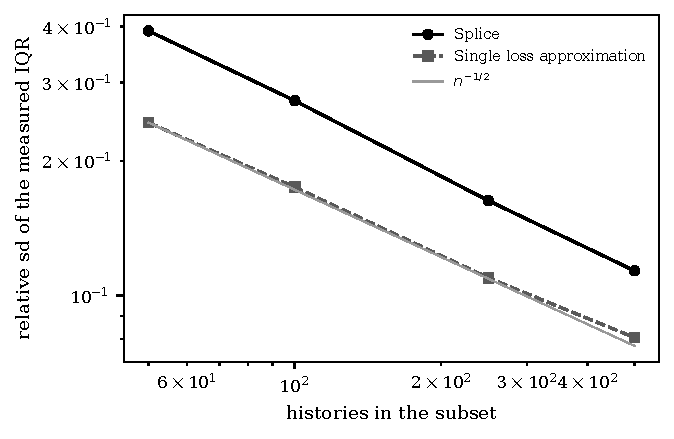
\includegraphics[width=0.62\textwidth]{precision-vs-histories.pdf}
\caption{Relative standard deviation of the measured interquartile range of the capital ratio over 400 random subsets of 50 to 500 of the 1{,}000 histories of a cell, median over the 16 cells, for the splice and the single loss approximation; the grey line is the $n^{-1/2}$ reference scaled to the first point.}
\label{fig:precision}
\end{figure}

\subsection{The main comparison}
\label{sec:res-main}

\Cref{tab:main-results} gives, for each of the 16 cells, the splice and the single loss approximation as multiples of the true quantile, with 95 percent bootstrap intervals over the 1{,}000 histories. The splice is defined on \cSpDTaNdef{} to \cSpATaNdef{} of the 1{,}000 histories of a cell, and \cref{fig:iqr-by-cell} plots its interquartile range, with the interval, against the tail index for the four cells. The interquartile range of the splice capital lies between \spIqrMin{} and \spIqrMax{} times the true quantile:
the smallest value is at $\xi=0.6$ with 10 years and a threshold of EUR 20,000, where the interval is \cSpATbIqrLo{} to \cSpATbIqrHi{}, and the largest is at $\xi=0.96$ with 5 years and EUR 20,000. The same table shows a median ratio between \cSpDFaMed{} and \cSpCTbMed{} for the splice, so the splice both understates the truth in the typical history and disperses by a multiple of it.
For the single loss approximation, which is defined on every history, the interquartile range is between \cSlATaIqr{} and \cSlDFbIqr{}, roughly half of the splice's, and the share of histories below the truth is 50 to 63 percent.

\begin{table}[htbp]
\centering\scriptsize
\caption{The 99.9 percent capital of the lognormal-GPD splice and of the single loss approximation as a multiple of the true quantile, in the 16 cells of 1{,}000 independent histories each: the histories on which the splice is defined, the median ratio, the interquartile range of the ratio with its 95 percent percentile bootstrap interval over the histories (2{,}000 resamples), and the percentage of histories below the truth. The single loss approximation is defined on every history.}
\label{tab:main-results}
\fitwidth{\begin{tabular}{rrrr|rrr|rrr}
\toprule
 & & & \multicolumn{4}{c|}{Splice} & \multicolumn{3}{c}{Single loss approximation} \\
$\xi$ & Years & $H$ (EUR k) & Defined & Median & IQR [95\% CI] & Below 1 (\%) & Median & IQR [95\% CI] & Below 1 (\%) \\
\midrule
0.6 & 5 & 10 & 959 & 0.76 & 1.95 [1.67, 2.29] & 56 & 0.84 & 1.03 [0.96, 1.13] & 58 \\
0.6 & 5 & 20 & 771 & 0.76 & 2.03 [1.68, 2.39] & 58 & 0.84 & 1.10 [1.01, 1.24] & 57 \\
0.6 & 10 & 10 & 996 & 0.85 & 1.43 [1.25, 1.59] & 56 & 0.84 & 0.69 [0.61, 0.76] & 61 \\
0.6 & 10 & 20 & 859 & 0.84 & 1.35 [1.13, 1.61] & 57 & 0.80 & 0.73 [0.67, 0.79] & 63 \\
\midrule
0.8 & 5 & 10 & 904 & 0.66 & 2.74 [2.23, 3.09] & 59 & 0.92 & 1.28 [1.18, 1.44] & 54 \\
0.8 & 5 & 20 & 682 & 0.64 & 2.56 [2.15, 3.42] & 60 & 0.90 & 1.53 [1.38, 1.76] & 54 \\
0.8 & 10 & 10 & 971 & 0.82 & 1.78 [1.54, 2.11] & 55 & 0.93 & 0.82 [0.70, 0.90] & 54 \\
0.8 & 10 & 20 & 727 & 0.91 & 1.98 [1.71, 2.24] & 53 & 0.96 & 1.02 [0.91, 1.14] & 52 \\
\midrule
0.96 & 5 & 10 & 725 & 0.78 & 3.10 [2.29, 3.87] & 57 & 0.94 & 1.34 [1.19, 1.56] & 53 \\
0.96 & 5 & 20 & 550 & 0.63 & 3.30 [2.44, 4.70] & 56 & 0.90 & 1.74 [1.50, 1.94] & 54 \\
0.96 & 10 & 10 & 818 & 0.76 & 2.11 [1.76, 2.54] & 55 & 0.97 & 0.90 [0.78, 0.99] & 52 \\
0.96 & 10 & 20 & 572 & 0.93 & 2.23 [1.83, 2.58] & 53 & 0.97 & 1.18 [1.05, 1.29] & 51 \\
\midrule
1.1 & 5 & 10 & 229 & 0.50 & 3.30 [2.39, 5.26] & 57 & 0.95 & 1.32 [1.18, 1.48] & 52 \\
1.1 & 5 & 20 & 443 & 0.72 & 3.18 [2.56, 4.60] & 55 & 0.84 & 1.78 [1.50, 1.98] & 55 \\
1.1 & 10 & 10 & 128 & 0.89 & 1.68 [1.32, 3.32] & 52 & 0.94 & 0.95 [0.87, 1.03] & 53 \\
1.1 & 10 & 20 & 409 & 0.73 & 2.32 [1.90, 2.78] & 57 & 1.00 & 1.44 [1.29, 1.63] & 50 \\
\bottomrule
\end{tabular}}
\end{table}


\begin{figure}[htbp]
\centering
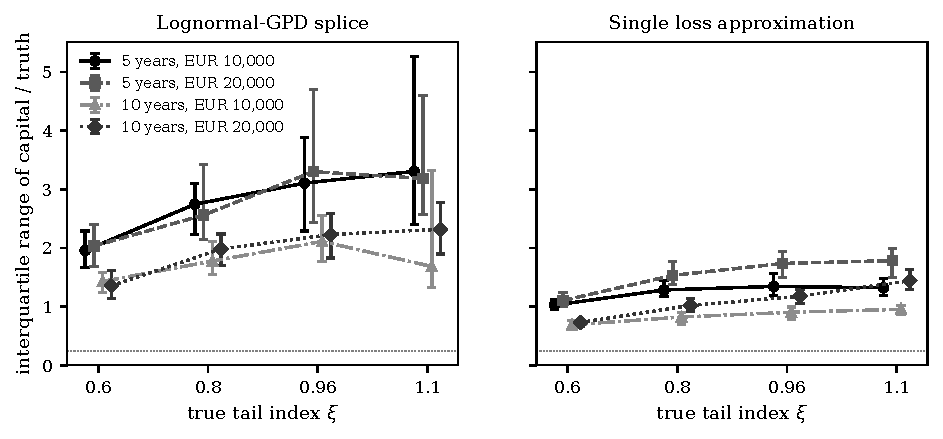
\includegraphics[width=0.95\textwidth]{iqr-by-cell.pdf}
\caption{Interquartile range of the capital divided by the true quantile against the true tail index for the splice (left) and the single loss approximation (right), in the four combinations of history length and collection threshold, with 95 percent bootstrap intervals over 1{,}000 histories; the dotted line is the green limit 0.25 of the product.}
\label{fig:iqr-by-cell}
\end{figure}

\Cref{fig:ecdf} shows the distribution of the ratio itself for four rungs in the cell of 10 years and EUR 20,000. The curves are wide on a logarithmic axis: at $\xi=0.96$ the 5th and the 95th percentiles of the splice ratio are \cSpCTbPlo{} and \cSpCTbPhi{}, a factor of more than one hundred, and the share of histories within a factor of two of the truth is only \plSpWithin{} percent for the splice over all cells, against \plSlWithin{} for the single loss approximation and \plScWithin{} for the scenario combination.

\begin{figure}[htbp]
\centering
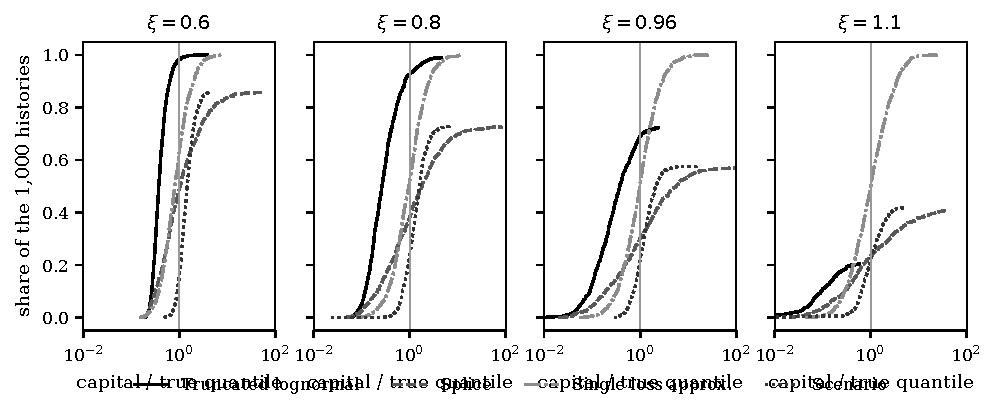
\includegraphics[width=\textwidth]{ecdf-ratio.pdf}
\caption{Cumulative share of the 1{,}000 histories of the cell of 10 years and threshold EUR 20,000 whose capital divided by the true quantile is at most the abscissa, for the truncated lognormal, the splice, the single loss approximation and the scenario combination, at the four tail indices; a curve ends below one where the rung is undefined on the remaining histories, and the vertical line marks the truth.}
\label{fig:ecdf}
\end{figure}

\subsection{The ladder}
\label{sec:res-ladder}

\Cref{tab:rungs} summarises the ten rungs over the 16 cells and \cref{fig:iqr-by-rung} plots their interquartile ranges at the shortest and the longest history. No rung is stable. The lognormal that ignores the threshold has a very small interquartile range, \plLgIqr{} on average, because its error is systematic: its median capital is \cLgATbMed{} of the truth at $\xi=0.6$ and \cLgDTbMed{} at $\xi=1.1$,
and practically no history (\plLgWithin{} percent) falls within a factor of two of the truth. The truncated lognormal removes part of that bias, and is defined on only \plTrDef{} percent of the histories, \cTrDTaNdef{} of the 1{,}000 at $\xi=1.1$ with 10 years and EUR 10,000. The scenario combination has a mean interquartile range of \plScIqr{}, comparable with the mean-adjusted fits (\plMaIqr{}, \plObIqr{} and \plCvIqr{} for the maximum likelihood, bias-robust and Cram\'er-von Mises fits), and the highest share within a factor of two, \plScWithin{} percent, but its prior is the expert's true severity quantile of the generator, rounded to two significant figures, so it measures what an informative prior is worth and not an estimate from data.

\begin{table}[htbp]
\centering\small
\caption{The ten estimation rungs over the 16 cells: the share of the 16{,}000 histories on which the rung returns a capital, the mean over cells of the median ratio to the truth, the range over cells of the interquartile range of the ratio, the share of defined histories within a factor of two of the truth with its Wilson 95 percent interval, and the number of cells on which the capital stability test is red.}
\label{tab:rungs}
\fitwidth{\begin{tabular}{lrrrrr}
\toprule
Rung & Defined (\%) & Mean median & IQR range over cells & Within factor 2 (\%) [95\% CI] & Red cells \\
\midrule
Lognormal, threshold ignored & 100 & 0.06 & 0.00 to 0.03 & 0.0 [0.0, 0.0] & 16 of 16 \\
Truncated lognormal & 74 & 0.20 & 0.05 to 0.35 & 14.8 [14.2, 15.5] & 16 of 16 \\
Lognormal-GPD splice & 67 & 0.76 & 1.35 to 3.30 & 34.0 [33.1, 34.9] & 16 of 16 \\
Single loss approximation & 100 & 0.91 & 0.69 to 1.78 & 57.2 [56.4, 57.9] & 16 of 16 \\
Single loss approximation, mean correction & 66 & 0.85 & 0.56 to 1.32 & 65.5 [64.5, 66.4] & 12 of 12 \\
Scenario combination & 68 & 1.18 & 0.51 to 1.23 & 82.3 [81.6, 83.0] & 16 of 16 \\
\midrule
Mean-adjusted single loss approximation & 71 & 0.70 & 0.12 to 1.31 & 61.6 [60.7, 62.5] & 16 of 16 \\
Cram\'er-von Mises GPD & 70 & 0.65 & 0.13 to 1.85 & 46.8 [45.9, 47.8] & 16 of 16 \\
Optimally bias-robust GPD & 70 & 0.71 & 0.12 to 1.48 & 59.6 [58.7, 60.5] & 16 of 16 \\
Cram\'er-von Mises lognormal & 72 & 0.13 & 0.06 to 0.26 & 8.3 [7.8, 8.8] & 16 of 16 \\
\bottomrule
\end{tabular}}
\end{table}


\begin{figure}[htbp]
\centering
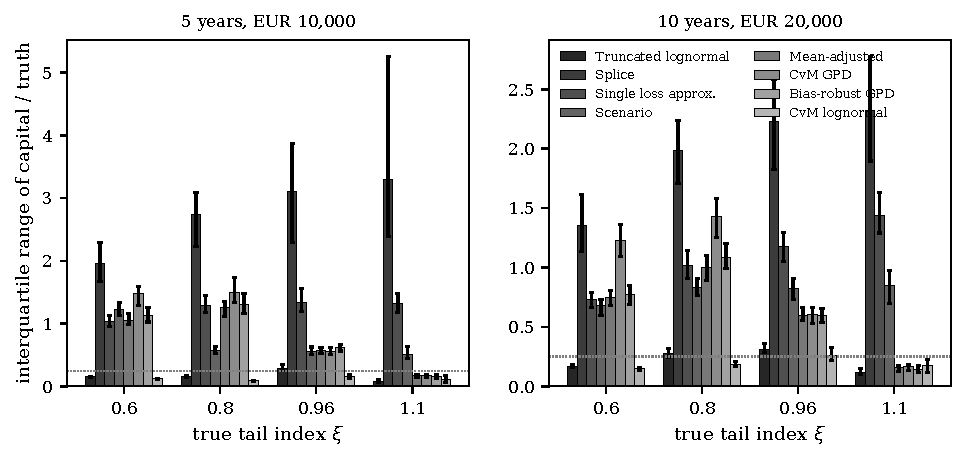
\includegraphics[width=\textwidth]{iqr-by-rung.pdf}
\caption{Interquartile range of the capital divided by the true quantile by estimation rung and tail index, in the cell of 5 years and threshold EUR 10,000 (left) and in the cell of 10 years and threshold EUR 20,000 (right), with 95 percent bootstrap intervals; the dotted line is the green limit 0.25 of the product.}
\label{fig:iqr-by-rung}
\end{figure}

\Cref{tab:lights} counts the lights of the capital stability test: every rung is red in every cell where it is defined, \redTotal{} of \redTotal{} rows, and \redSix{} of \rowsSix{} on the six-rung ladder. The test combines the interquartile range and the bias, so a rung may be red for either reason; the lognormals, which understate the truth by a large margin, fail on bias, and the splice, the single loss approximation and the scenario combination fail on dispersion.

\begin{table}[htbp]
\centering\small
\caption{The lights of the capital stability test over the 16 cells for each rung, against the limits of 0.25 and 0.50 on the interquartile range of the ratio and 0.10 and 0.25 on the absolute bias: the number of cells in which each rung is green, amber and red, from the committed documents. The last row, the mean-corrected single loss approximation, is a comparison only and is in no count of the text; it is computed on 12 cells.}
\label{tab:lights}
\begin{tabular}{lrrr}
\toprule
Rung & Green & Amber & Red \\
\midrule
Lognormal, threshold ignored & 0 & 0 & 16 \\
Truncated lognormal & 0 & 0 & 16 \\
Lognormal-GPD splice & 0 & 0 & 16 \\
Single loss approximation & 0 & 0 & 16 \\
Scenario combination & 0 & 0 & 16 \\
Mean-adjusted single loss approximation & 0 & 0 & 16 \\
Cram\'er-von Mises GPD & 0 & 0 & 16 \\
Optimally bias-robust GPD & 0 & 0 & 16 \\
Cram\'er-von Mises lognormal & 0 & 0 & 16 \\
\midrule
\multicolumn{4}{l}{\emph{Comparison only, in no count of the text (form not confirmed)}} \\
Single loss approximation, mean correction & 0 & 0 & 12 \\
\bottomrule
\end{tabular}
\end{table}


\subsection{Bias}
\label{sec:res-bias}

\Cref{fig:median} plots the median ratio, averaged over the four cells of each tail index. The single loss approximation has a mean median of \plSlMed{}, below one in \slBelowCells{} of the 16 cells, and it approaches one as the tail gets heavier; this follows the gap of the approximation at the true parameters, \slGapA{} percent at $\xi=0.6$ and \slGapD{} percent at $\xi=1.1$ (\cref{sec:theory-conditions}).
The splice has a mean median of \plSpMed{}, further from one at every tail index, and the scenario combination overshoots, with \plScMed{}. The median is a statement about the typical history and says nothing about a single bank, whose ratio is spread as in \cref{fig:ecdf}.

\begin{figure}[htbp]
\centering
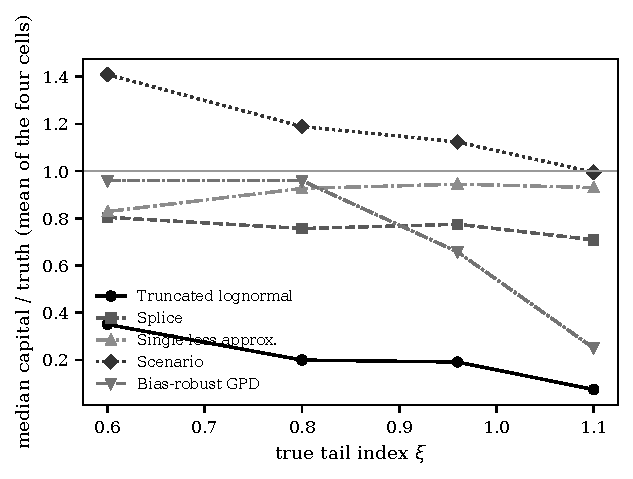
\includegraphics[width=0.62\textwidth]{median-by-xi.pdf}
\caption{Median capital divided by the true quantile against the true tail index for five rungs, averaged over the four cells of each index in which the rung is defined; the horizontal line marks the truth at one.}
\label{fig:median}
\end{figure}

The bias of the splice and of the scenario combination is not a defect of estimation alone. The splice conditions on a fit that succeeds, and the scenario combination takes its tail from the prior, so each has a different relation to the truth than the single loss approximation, whose target is the closed form of the tail.

\subsection{Histories on which a rung is undefined}
\label{sec:res-undefined}

The engine refuses a fit it cannot make, and the refusal is counted. The splice is defined on \plSpDef{} percent of the 16{,}000 histories and the scenario combination on \plScDef{} percent, and the number varies by cell from \cSpDTaNdef{} of 1{,}000 (splice, $\xi=1.1$, 10 years, EUR 10,000) to 996. The truncated lognormal and the splice fail most often where the tail is heaviest, and more often at the lower threshold, because the maximum likelihood fit of a lognormal to Pareto-like data can run to a degenerate maximum.
The statistics of these rungs are conditional on the fit succeeding, and the conditioning flatters them: a history on which the fit fails is exactly one in which the capital would have been furthest from the truth. The single loss approximation is defined on every history and its dispersion is unconditional.

The count of undefined histories is itself a result for a validator. A method that returns a capital on fewer than half of the histories of a bank-like process at the heavy tails cannot be applied to a given bank without a fallback, and a fallback changes the statistics reported here.

\subsection{The wrong conclusion about the mean}
\label{sec:res-mean}

\Cref{tab:tail-index} and \cref{fig:infinite} report the tail index fitted above the collection threshold. At $\xi=0.96$ the share of histories with $\hat\xi\ge1$ is between \infLo{} and \infHi{} percent over the four cells: roughly one history in three concludes that the mean does not exist when it does. At $\xi=1.1$ the share that concludes a finite mean is between \finLo{} and \finHi{} percent.
The median fitted index at $\xi=0.96$ and 5 years is \cXiCFaMed{}, within the error of the true value, so the wrong conclusion is a property of the spread of the fit and not of a bias. Fitting above two, four and eight times the threshold leaves fewer exceedances and moves the share toward one half (columns $2H$ to $8H$ of \cref{tab:tail-index}), which is the behaviour a threshold-stability plot shows and why the plot cannot settle the question at these sample sizes.

\begin{table}[htbp]
\centering\scriptsize
\caption{The tail index fitted above the collection threshold in each cell: the histories with a fit, the median and the 5th to 95th percentiles of the fitted index, the percentage of histories whose index is 1 or more with its Wilson 95 percent interval, the percentage predicted by the normal approximation of the maximum likelihood estimator, and the measured percentage when the fit is made above two, four and eight times the threshold.}
\label{tab:tail-index}
\fitwidth{\begin{tabular}{rrrrrrrrrr}
\toprule
$\xi$ & Years & $H$ (EUR k) & Fits & Median $\hat\xi$ [5\%, 95\%] & $\hat\xi\ge1$ (\%) [95\% CI] & Predicted (\%) & $2H$ & $4H$ & $8H$ \\
\midrule
0.6 & 5 & 10 & 1000 & 0.60 [0.44, 0.75] & 0.0 [0.0, 0.4] & 0.0 & 0 & 0 & 3 \\
0.6 & 5 & 20 & 1000 & 0.59 [0.42, 0.78] & 0.0 [0.0, 0.4] & 0.0 & 0 & 2 & 9 \\
0.6 & 10 & 10 & 1000 & 0.60 [0.48, 0.70] & 0.0 [0.0, 0.4] & 0.0 & 0 & 0 & 0 \\
0.6 & 10 & 20 & 1000 & 0.59 [0.47, 0.73] & 0.0 [0.0, 0.4] & 0.0 & 0 & 0 & 5 \\
\midrule
0.8 & 5 & 10 & 1000 & 0.80 [0.63, 0.96] & 2.4 [1.6, 3.5] & 2.2 & 5 & 12 & 18 \\
0.8 & 5 & 20 & 1000 & 0.79 [0.57, 1.01] & 6.3 [5.0, 8.0] & 5.6 & 11 & 16 & 23 \\
0.8 & 10 & 10 & 1000 & 0.80 [0.69, 0.92] & 0.5 [0.2, 1.2] & 0.2 & 2 & 5 & 11 \\
0.8 & 10 & 20 & 1000 & 0.80 [0.65, 0.94] & 1.2 [0.7, 2.1] & 1.2 & 4 & 9 & 20 \\
\midrule
0.96 & 5 & 10 & 1000 & 0.95 [0.80, 1.13] & 33.2 [30.4, 36.2] & 34.8 & 37 & 38 & 38 \\
0.96 & 5 & 20 & 1000 & 0.95 [0.73, 1.18] & 34.4 [31.5, 37.4] & 38.5 & 37 & 35 & 38 \\
0.96 & 10 & 10 & 1000 & 0.96 [0.84, 1.07] & 26.8 [24.1, 29.6] & 29.0 & 32 & 35 & 36 \\
0.96 & 10 & 20 & 1000 & 0.96 [0.79, 1.12] & 31.7 [28.9, 34.6] & 34.0 & 37 & 40 & 36 \\
\midrule
1.1 & 5 & 10 & 1000 & 1.09 [0.92, 1.26] & 81.8 [79.3, 84.1] & 83.8 & 72 & 66 & 57 \\
1.1 & 5 & 20 & 1000 & 1.08 [0.84, 1.33] & 73.2 [70.4, 75.9] & 75.2 & 64 & 57 & 53 \\
1.1 & 10 & 10 & 1000 & 1.09 [0.98, 1.21] & 91.2 [89.3, 92.8] & 91.8 & 82 & 71 & 66 \\
1.1 & 10 & 20 & 1000 & 1.10 [0.93, 1.27] & 83.6 [81.2, 85.8] & 83.3 & 76 & 67 & 59 \\
\bottomrule
\end{tabular}}
\end{table}


\begin{figure}[htbp]
\centering
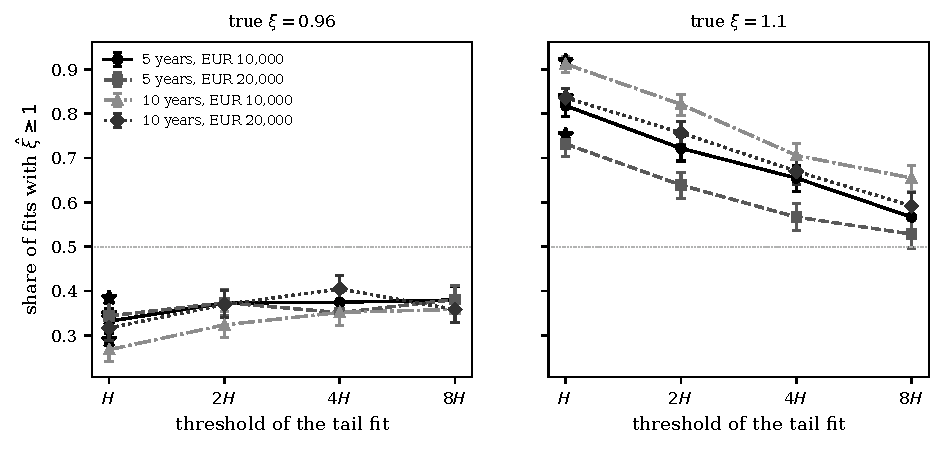
\includegraphics[width=0.95\textwidth]{infinite-mean-share.pdf}
\caption{Share of histories whose fitted tail index is one or more against the threshold of the tail fit, from the collection threshold $H$ to eight times it, for true tail indices 0.96 (left) and 1.1 (right) in the four cells, with Wilson 95 percent intervals; stars mark the share predicted at $H$ by the normal approximation of the theory.}
\label{fig:infinite}
\end{figure}

In no cell of the design is the share of false infinite-mean conclusions at 0.96 below \infLo{} percent, so there is no combination of the lengths and thresholds studied in which a validator can rule out the wrong side of the boundary.

\subsection{The theory against the measurement}
\label{sec:res-theory}

\Cref{tab:theory} and \cref{fig:theory} set the delta-method dispersion of \cref{eq:dispersion} against the measured standard deviation of the logarithm of the ratio of the single loss approximation. The prediction is within \thSdMaxErr{} percent in every cell and its mean error over cells is \thSdMeanErr{} percent, well inside the tolerance of \preSd{} percent of H5.
The interquartile range predicted from the lognormal approximation of the ratio is less accurate: it exceeds the measured one in \thIqrOver{} of the 16 cells, by \thIqrMean{} percent on average and up to \thIqrMaxErr{} percent, because the distribution of the logarithm of the ratio is more peaked than a normal one. The share of histories with $\hat\xi\ge1$ predicted by \cref{eq:misclassification} is within \thShareMaxErr{} points of the measured share in the cells at 0.96 and 1.1, inside the tolerance of \preShare{} points of H6, and it is slightly above the measured share in most cells, as the right panel of \cref{fig:theory} shows.
The same formula gives the history that would bring the interquartile range to 0.25 (\cref{fig:years}): \yrsMin{} years at the lightest tail and shortest threshold and \yrsMax{} years at $\xi=1.1$ with a threshold of EUR 20,000, an order of magnitude more than the 5 or 10 years of a bank.

\begin{table}[htbp]
\centering\scriptsize
\caption{The dispersion of the single loss approximation predicted by the delta method at the true parameters against the dispersion measured over the 1{,}000 histories of each cell: the expected number of recorded losses $k$, the standard deviation of the logarithm of the ratio, measured and predicted, the relative error of the prediction in percent, the interquartile range of the ratio, measured and predicted by a lognormal of the predicted dispersion, and the years of history at which the predicted interquartile range reaches 0.25.}
\label{tab:theory}
\fitwidth{\begin{tabular}{rrrrrrrrrr}
\toprule
$\xi$ & Years & $H$ (EUR k) & $k$ & $\mathrm{sd}$ measured & $\mathrm{sd}$ predicted & Error (\%) & IQR measured & IQR predicted & Years for 0.25 \\
\midrule
0.6 & 5 & 10 & 296 & 0.810 & 0.815 & +0.7 & 1.03 & 1.16 & 97 \\
0.6 & 5 & 20 & 205 & 0.939 & 0.939 & +0.0 & 1.10 & 1.35 & 129 \\
0.6 & 10 & 10 & 592 & 0.596 & 0.577 & -3.2 & 0.69 & 0.80 & 97 \\
0.6 & 10 & 20 & 410 & 0.645 & 0.664 & +3.0 & 0.73 & 0.93 & 129 \\
\midrule
0.8 & 5 & 10 & 326 & 0.954 & 0.930 & -2.5 & 1.28 & 1.34 & 127 \\
0.8 & 5 & 20 & 205 & 1.171 & 1.116 & -4.7 & 1.53 & 1.65 & 182 \\
0.8 & 10 & 10 & 653 & 0.644 & 0.658 & +2.1 & 0.82 & 0.92 & 127 \\
0.8 & 10 & 20 & 410 & 0.791 & 0.789 & -0.3 & 1.02 & 1.11 & 182 \\
\midrule
0.96 & 5 & 10 & 367 & 0.995 & 0.993 & -0.2 & 1.34 & 1.44 & 144 \\
0.96 & 5 & 20 & 205 & 1.241 & 1.249 & +0.6 & 1.74 & 1.89 & 228 \\
0.96 & 10 & 10 & 734 & 0.691 & 0.702 & +1.6 & 0.90 & 0.98 & 144 \\
0.96 & 10 & 20 & 410 & 0.871 & 0.883 & +1.4 & 1.18 & 1.26 & 228 \\
\midrule
1.1 & 5 & 10 & 429 & 1.016 & 1.017 & +0.1 & 1.32 & 1.48 & 151 \\
1.1 & 5 & 20 & 205 & 1.355 & 1.363 & +0.6 & 1.78 & 2.11 & 272 \\
1.1 & 10 & 10 & 857 & 0.716 & 0.719 & +0.5 & 0.95 & 1.01 & 151 \\
1.1 & 10 & 20 & 410 & 0.955 & 0.963 & +0.9 & 1.44 & 1.39 & 272 \\
\bottomrule
\end{tabular}}
\end{table}


\begin{figure}[htbp]
\centering
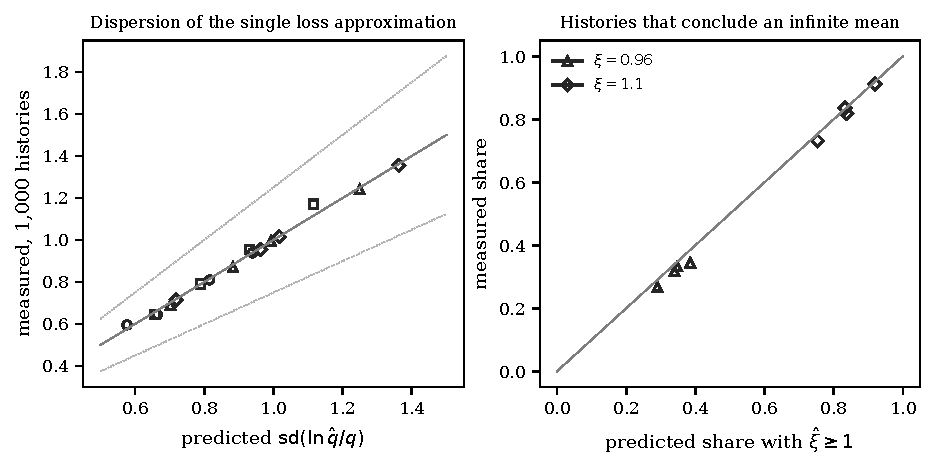
\includegraphics[width=0.95\textwidth]{theory-vs-measured.pdf}
\caption{Measured against predicted standard deviation of the logarithm of the capital ratio of the single loss approximation in the 16 cells, with lines at equality and at plus and minus 25 percent (left), and measured against predicted share of histories with a fitted tail index of one or more at indices 0.96 and 1.1 (right).}
\label{fig:theory}
\end{figure}

\begin{figure}[htbp]
\centering
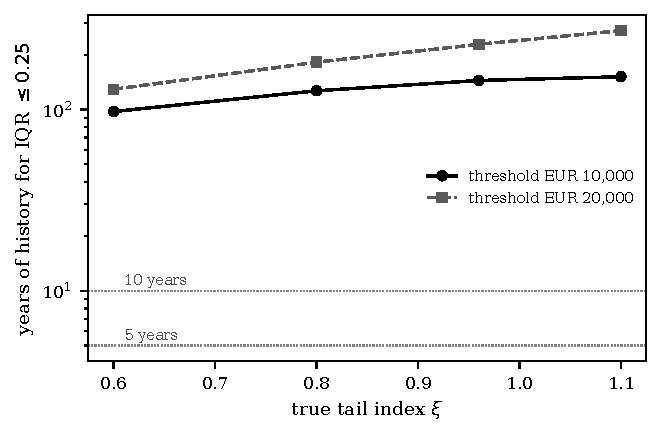
\includegraphics[width=0.62\textwidth]{years-for-green.pdf}
\caption{Years of history at which the predicted interquartile range of the single loss approximation reaches the green limit 0.25 of the product, against the true tail index for the two collection thresholds, on a logarithmic axis; the dotted lines mark the 5 and 10 years of the experiment.}
\label{fig:years}
\end{figure}

\subsection{The standardised approach}
\label{sec:res-sma}

\Cref{tab:sma} gives the capital of the standardised approach as a multiple of the true quantile. It is stable across histories relative to its own level, because it depends on the losses only through the average annual loss and enters the multiplier with the exponent 0.8, and it does not track the tail: its median is \smaA{} times the true quantile at $\xi=0.6$, \smaB{} at 0.8, \smaC{} at 0.96 and \smaD{} at 1.1 in the cell of 10 years and EUR 20,000.
The approach is not calibrated to the 99.9 percent quantile of any bank, so the ratio is a comparison and not an error; it shows that the standardised capital is neither a conservative nor an aggressive proxy for the quantile of this process, but a quantity that does not move with the tail that the quantile follows.

\begin{table}[htbp]
\centering\small
\caption{The standardised approach against the true quantile in the 16 cells: the median over the 1{,}000 histories of the operational risk capital divided by the true 99.9 percent quantile, its first and third quartiles, its interquartile range and the median capital in EUR million, at the business indicator component of EUR 180 million of the synthetic bank.}
\label{tab:sma}
\begin{tabular}{rrrrrrr}
\toprule
$\xi$ & Years & $H$ (EUR k) & Median ratio & Quartiles & IQR & Median capital (EUR m) \\
\midrule
0.6 & 5 & 10 & 4.022 & 3.941 to 4.120 & 0.179 & 136.3 \\
0.6 & 5 & 20 & 3.967 & 3.890 to 4.073 & 0.183 & 134.5 \\
0.6 & 10 & 10 & 4.030 & 3.967 to 4.111 & 0.144 & 136.6 \\
0.6 & 10 & 20 & 3.975 & 3.906 to 4.053 & 0.147 & 134.7 \\
\midrule
0.8 & 5 & 10 & 0.873 & 0.846 to 0.921 & 0.075 & 142.7 \\
0.8 & 5 & 20 & 0.859 & 0.829 to 0.901 & 0.071 & 140.4 \\
0.8 & 10 & 10 & 0.882 & 0.857 to 0.915 & 0.058 & 144.1 \\
0.8 & 10 & 20 & 0.869 & 0.843 to 0.908 & 0.064 & 142.0 \\
\midrule
0.96 & 5 & 10 & 0.239 & 0.227 to 0.258 & 0.031 & 151.6 \\
0.96 & 5 & 20 & 0.233 & 0.221 to 0.254 & 0.033 & 147.7 \\
0.96 & 10 & 10 & 0.242 & 0.231 to 0.261 & 0.030 & 153.6 \\
0.96 & 10 & 20 & 0.239 & 0.227 to 0.258 & 0.031 & 151.6 \\
\midrule
1.1 & 5 & 10 & 0.076 & 0.070 to 0.085 & 0.015 & 162.4 \\
1.1 & 5 & 20 & 0.074 & 0.068 to 0.083 & 0.015 & 158.5 \\
1.1 & 10 & 10 & 0.078 & 0.072 to 0.088 & 0.016 & 167.2 \\
1.1 & 10 & 20 & 0.077 & 0.071 to 0.087 & 0.016 & 165.0 \\
\bottomrule
\end{tabular}
\end{table}


\subsection{Whether each hypothesis held}
\label{sec:res-hypotheses}

\Cref{tab:hypotheses} lists the six predictions of \cref{sec:ed-hypotheses} with the measured values. All six held. H1 holds at two decimals, with a range of \spIqrMin{} to \spIqrMax{}; the bootstrap interval of the smallest cell, \cSpATbIqrLo{} to \cSpATbIqrHi{}, shows that the endpoints of the range are themselves uncertain by tenths of the truth. H2 holds on the six-rung ladder and on the four additional rungs.
H3 and H4 hold with the ranges \infLo{} to \infHi{} and \finLo{} to \finHi{} percent, which round to the stated 27 to 34 and 9 to 27 at the whole percent. H5 and H6 hold with the errors in the table. The agreement of the delta-method dispersion with the measurement is closer than the sampling noise of the measurement in several cells, so the data cannot separate the prediction from a slightly different formula; the evidence is that the formula is adequate for the purpose of finding the history needed, not that it is exact.

\begin{table}[htbp]
\centering\small
\caption{The six predictions stated before the measurements, the value measured on the 16{,}000 histories, and whether each held. H1 to H4 are the quantitative statements of the measurement; H5 and H6 are the predictions of the theory, with the tolerances fixed before they were compared with the 16 cells.}
\label{tab:hypotheses}
\begin{tabularx}{\textwidth}{lXXl}
\toprule
Id & Prediction & Measured & Outcome \\
\midrule
H1 & The interquartile range of the splice capital over the true quantile lies between 1.35 and 3.30 in the 16 cells & 1.3536 to 3.3038 & Held \\
H2 & Every capital stability row of the six-rung ladder is red & 92 of 92 rows red (156 of 156 with the four robust rungs) & Held \\
H3 & 27 to 34 percent (whole percent) of the histories at $\xi=0.96$ conclude an infinite mean & 26.8 to 34.4 percent & Held \\
H4 & 9 to 27 percent (whole percent) of the histories at $\xi=1.1$ conclude a finite mean & 8.8 to 26.8 percent & Held \\
H5 & The delta-method dispersion of the single loss approximation is within 25 percent of the measured one in every cell & largest relative error 4.7 percent & Held \\
H6 & The predicted share of histories with $\hat\xi\ge1$ is within 5 points of the measured one in every cell at $\xi=0.96$ and $1.1$ & largest absolute error 4.1 points & Held \\
\bottomrule
\end{tabularx}
\end{table}


\section{Ablation}
\label{sec:ablation}

The ablation asks what each component of the estimation ladder contributes, and what the design variables of the protocol contribute, on the same histories. A component is compared with the rung just before it on the histories where both return a capital, so the comparison is paired and is not confounded by the histories on which a rung fails.

\subsection{Components of the estimation ladder}
\label{sec:abl-components}

\Cref{tab:ablation} and \cref{fig:ablation} give, for each component, the share of paired histories within a factor of two of the truth before and after, the change with its 95 percent bootstrap interval, and the standard deviation of the logarithm of the ratio.
Modelling the collection threshold lifts the share within a factor of two from \abThresholdFrom{} to \abThresholdTo{} percent, a gain of \abThresholdDelta{} points (interval \abThresholdLo{} to \abThresholdHi{}) over \abThresholdN{} paired histories: it is necessary, because ignoring it puts the median capital at \cLgATbMed{} of the truth at $\xi=0.6$ and at \cLgDTbMed{} at $\xi=1.1$, and far from sufficient.
Splicing a generalised Pareto tail onto the lognormal body adds \abHeavytailDelta{} points (\abHeavytailFrom{} to \abHeavytailTo{} percent) but increases the dispersion of the logarithm of the ratio from 0.79 to 1.52: the splice removes bias and adds variance, because the tail has two parameters fitted only on the losses above EUR 100,000, a small part of the recorded history.
Replacing the aggregation of the splice by the closed-form single loss approximation on a generalised Pareto fit above the collection threshold adds \abClosedformDelta{} points and halves the dispersion of the logarithm, because the fit uses every recorded loss above the threshold instead of the few above the splice point; this is the largest gain among the components that read only the data.
The adjustment by one mean adds \abMeanadjustedDelta{} points (interval \abMeanadjustedLo{} to \abMeanadjustedHi{}), which is small but has an interval that excludes zero. It is refused wherever the fitted index is one or more and is compared over \abMeanadjustedCells{} cells, at 1.1 only on the histories whose fitted index is below one.
The mean correction is not read as a component, because its form is not confirmed against a primary text (\cref{sec:pm-ladder}). Its row, the last of \cref{tab:ablation} and set apart there, is a comparison on the \abMeancorrectionCells{} cells where it is computed (it is not computed for the variant whose true index is 1.1): it adds \abMeancorrectionDelta{} points (interval \abMeancorrectionLo{} to \abMeancorrectionHi{}). The two corrected capitals differ by exactly one mean of the fitted severity (\cref{eq:mean-corrections}) and agree on the same history to a median of \rFiveSevenMed{} percent, so the comparison row and the adjustment are one effect in two forms and are not added.

\begin{table}[htbp]
\centering\scriptsize
\caption{The ablation of the estimation ladder: for each component, the paired comparison on the histories of the 16 cells where both rungs return a capital, the share of those histories within a factor of two of the truth before and after, the change in percentage points with its 95 percent bootstrap interval over the paired histories, and the standard deviation of the logarithm of the ratio before and after. The last row is a comparison only, on the 12 cells where the mean-corrected rung is computed: its form is not confirmed against a primary text, so it is not read as a component of the ladder.}
\label{tab:ablation}
\fitwidth{\begin{tabular}{llrrrrr}
\toprule
Component & Rungs compared & Pairs & Before (\%) & After (\%) & Change (points) [95\% CI] & $\mathrm{sd}$ of $\ln$ ratio \\
\midrule
Model the collection threshold & Lognormal, threshold ignored to Truncated lognormal & 11{,}876 & 0.0 & 14.8 & +14.8 [+14.2, +15.5] & 1.24 to 0.86 \\
Splice a GPD tail onto the body & Truncated lognormal to Lognormal-GPD splice & 9{,}385 & 13.6 & 35.2 & +21.6 [+20.4, +22.9] & 0.79 to 1.52 \\
Closed-form tail instead of aggregation & Lognormal-GPD splice to Single loss approximation & 10{,}743 & 34.0 & 59.5 & +25.4 [+24.3, +26.6] & 1.63 to 0.87 \\
Replace the tail by the scenario credibility tail & Lognormal-GPD splice to Scenario combination & 10{,}743 & 34.0 & 82.5 & +48.5 [+47.3, +49.6] & 1.63 to 0.48 \\
Adjust the approximation by one mean & Single loss approximation to Mean-adjusted single loss approximation & 11{,}337 & 58.6 & 61.6 & +3.0 [+2.6, +3.4] & 0.84 to 0.82 \\
Fit the GPD by Cram\'er-von Mises & Mean-adjusted single loss approximation to Cram\'er-von Mises GPD & 10{,}371 & 62.2 & 47.6 & -14.6 [-15.7, -13.5] & 0.81 to 1.07 \\
Fit the GPD by the bias-robust estimator & Mean-adjusted single loss approximation to Optimally bias-robust GPD & 10{,}941 & 61.7 & 60.0 & -1.7 [-2.4, -1.0] & 0.82 to 0.86 \\
Fit a lognormal instead of the GPD & Cram\'er-von Mises GPD to Cram\'er-von Mises lognormal & 10{,}275 & 49.1 & 4.9 & -44.2 [-45.3, -43.1] & 1.05 to 0.91 \\
\midrule
\multicolumn{7}{l}{\emph{Comparison only, in no count of the text (form not confirmed)}} \\
Add the mean correction & Single loss approximation to Single loss approximation, mean correction & 10{,}635 & 62.5 & 65.5 & +2.9 [+2.5, +3.4] & 0.79 to 0.76 \\
\bottomrule
\end{tabular}}
\end{table}


\begin{figure}[htbp]
\centering
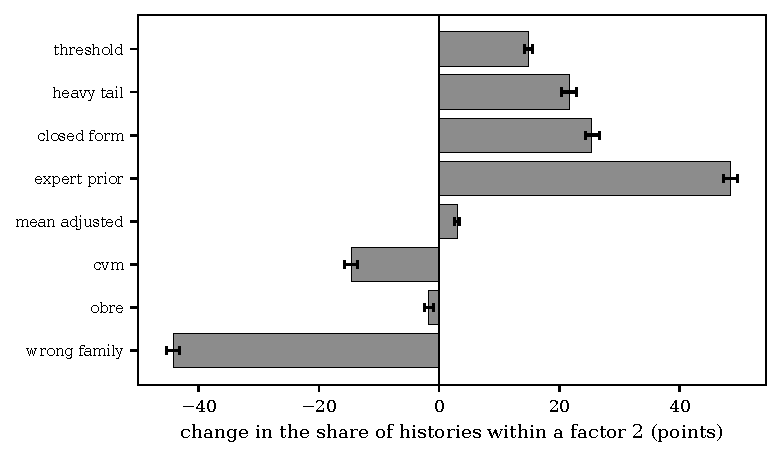
\includegraphics[width=0.78\textwidth]{ablation-change.pdf}
\caption{Change in the share of histories within a factor of two of the truth when each component of the estimation ladder is added, in percentage points with 95 percent bootstrap intervals over the paired histories of the 16 cells where both rungs return a capital; the comparison row of the mean-corrected rung is in \cref{tab:ablation} only.}
\label{fig:ablation}
\end{figure}

The scenario credibility tail adds \abExpertpriorDelta{} points over the splice, from \abExpertpriorFrom{} to \abExpertpriorTo{} percent, the largest change of the table. It is also the component that does not read the data: the prior of the Pareto shape is the expert's, the true severity quantiles of the generator rounded to two significant figures, so the gain measures what an accurate expert is worth to the estimate and not what the method extracts from a history. A biased expert would move the same rung the other way, and the experiment does not vary the expert.
The two robust fits do not help on this process. The minimum Cram\'er-von Mises fit lowers the share within a factor of two by \abCvmDown{} points (interval \abCvmDownLo{} to \abCvmDownHi{}) and raises the dispersion, as expected of a distance on the distribution function, which gives the largest losses, the ones that fix the tail, little weight, and the optimally bias-robust fit at an efficiency of 0.95 lowers it by \abObreDown{} points. The synthetic losses contain no contamination, so the protection of a robust estimator has nothing to protect against, and what remains is its loss of efficiency.
Fitting a lognormal instead of the generalised Pareto family drops the share within a factor of two to \abWrongfamilyTo{} percent: a misspecified family is the largest negative effect of the table and is not repaired by robustness.

\subsection{Length of the history and collection threshold}
\label{sec:abl-design}

Doubling the history from 5 to 10 years divides the standard deviation of the logarithm of the single loss approximation by \yrRatio{} on average over the eight pairs of cells (range \yrRatioMin{} to \yrRatioMax{}), which is the \sqrtTwo{} of the $1/\sqrt T$ law of \cref{cor:leading} to within the error of the measurement. Raising the collection threshold from EUR 10,000 to 20,000 removes between 31 and 52 percent of the median number of recorded losses (the expected numbers $k$ of \cref{tab:theory}), and multiplies the dispersion by \thrRatio{} on average (range \thrRatioMin{} to \thrRatioMax{}), in the direction and of the order that the $k^{-1/2}$ law of \cref{cor:leading} gives for the smaller number of recorded losses.
Neither variable brings any rung near the green limit, and the history that would is of the order of a century (\cref{fig:years}). The threshold is a modelling choice a bank makes, and the result says that the cost of a higher threshold is a larger dispersion even when the truncation is modelled correctly.

The two effects combine multiplicatively in the theory, so that a bank with ten years and the lower threshold has the smallest dispersion of the four cells at every tail index.

\subsection{Number of histories}
\label{sec:abl-histories}

The number of histories per cell is a component of the protocol. With 50 histories the relative standard deviation of the measured interquartile range of the splice is \subSpFifty{} percent and with 250 it is \subSpTwoFifty{}, and it falls close to the $n^{-1/2}$ law (\cref{fig:precision}); with the 1{,}000 histories of the experiment the bootstrap relative standard deviation is \bootSpMed{} percent for the splice (\bootSpMin{} to \bootSpMax{} across cells) and the intervals of \cref{tab:main-results} separate the lightest tail from the heaviest ones but, for the splice, overlap between neighbouring cells at the same tail index.

The number of histories is a cost and not only a precision. The 16 cells took about 70 minutes on ten processes, and the cost grows linearly with the number of histories while the precision improves as its inverse square root: halving the relative standard deviation of \subSpFiveHundred{} percent of the measured interquartile range of the splice at 500 histories would take four times as many histories. The number of histories is fixed by the design at 1{,}000 and no stopping rule is applied; at that number the interval of the interquartile range at the heavy tails is still wide, and the protocol reports the interval so that the reader sees the remaining uncertainty and not a point value that seems precise. A study of a single cell could draw many more histories at the cost of the other cells.

\section{Discussion}
\label{sec:discussion}

\subsection{Why the capital is unstable}
\label{sec:disc-why}

The instability is the arithmetic of extrapolation. A capital at the level 0.999 of an annual loss with \lamMin{} to \lamMax{} losses a year above the floor (\cref{tab:truth}) lies at the quantile of the severity of order $1-\tailOrderLo\times10^{-5}$ to $1-\tailOrderHi\times10^{-5}$, far beyond a history of a few hundred recorded losses, and the estimator reaches it through the tail index, which multiplies the logarithm of the extrapolation factor $L$.
\Cref{eq:leading} shows the consequence: the standard deviation of the logarithm of the capital is of order $(1+\xi)\,\ell/\sqrt k$ with $\ell\approx L-1/\xi$ between \ellMin{} and \ellMax{} in the 16 cells, so that a standard error of the fitted index of 0.1 becomes a standard deviation of the logarithm of the capital of almost one. The measurement and the theory agree to within \thSdMaxErr{} percent in all 16 cells, which means that the instability measured on the ladder is not a feature of one estimator or of one implementation: it is what an unbiased consistent estimator of the index does to a quantile that far out.
The other rungs differ from the single loss approximation in bias and in the use they make of the data, and the ablation shows how: the splice spends its parameters on the few losses above EUR 100,000 and pays in variance, the lognormal ignores the tail and pays in bias, and the scenario combination borrows the tail from an expert and gains because the expert is right.

\subsection{Which result is the most informative}
\label{sec:disc-informative}

The misclassification of the mean is the result with the most direct consequence. A validator who fits a generalised Pareto tail to five years of data at a process of index 0.96 finds an index of one or more in about one history in three (\infLo{} to \infHi{} percent), and the fitted index at 1.1 is below one in \finLo{} to \finHi{} percent of the histories. The fitted index is centred near the true value (a median of \cXiCFaMed{} at 0.96 and five years), so the validator cannot tell from the point estimate which side of the boundary the process is on, and the conclusion that the mean does not exist, which has practical consequences for the expected shortfall and for the mean-corrected approximation, flips with the history.
\Cref{prop:mean} says the same in advance: the band of indistinguishability of \exBandC{} around the boundary at five years is wider than the distance of 0.04 between 0.96 and one, so a history of that length cannot decide.

\subsection{What the standardised approach does and does not do}
\label{sec:disc-sma}

The standardised approach is the stable number: its interquartile range over histories is small against its level, and a validator who recomputes it from another history of the same bank gets nearly the same capital. The measurement shows what it buys and what it costs. The capital does not move with the tail index, so it is \smaA{} times the true quantile at $\xi=0.6$ and \smaD{} times at $\xi=1.1$ for this process, and the measurement makes no claim about its adequacy because the approach is not calibrated to the 99.9 percent quantile of any bank.
The comparison supports the argument of \citet{peters2016} that the standardised approach is insensitive to the risk of the bank, in the one sense that can be measured here, and it is consistent with the concern of the Basel Committee about the variability of risk-weighted assets under internal modelling \citep{bcbsd355}, in the sense that the measured dispersion is a source of variability even when every bank uses the same model; it does not show that either is the better capital, because their targets differ.

\subsection{Negative and partial results}
\label{sec:disc-negative}

Four results go against a hope. The hypothesis stated before the robust fits were run, that they beat the splice in spread and in bias, is not confirmed: it is inconclusive over the 16 cells (the bias count is \rhCvmBias{} and \rhObreBias{} of \rhCells{}) and refuted at the tail indices 0.96 and 1.1, partly because the mean-adjusted rungs are defined only where the fitted index is below one (\cref{sec:res-hypotheses}). The robust fits do not help on clean data of the assumed family: the Cram\'er-von Mises fit lowers the share within a factor of two by \abCvmDown{} points and the bias-robust fit by \abObreDown{}; the benefit that \citet{opdyke2012} expect from them is protection against contamination, which the synthetic losses do not contain, so the experiment cannot confirm or refute that benefit. The mean correction changes the share within a factor of two by only \abMeancorrectionDelta{} points, and its form was not confirmed against a primary text.
And the splice, the rung of the loss distribution approach that a practitioner would consider the most complete, is the worst of the ladder after the three lognormal rungs on the share within a factor of two, \plSpWithin{} percent, because it conditions on a fit that fails on up to \spUndMax{} of 1{,}000 histories and has the largest dispersion where it succeeds.

One partial result concerns the interquartile range. The prediction from a lognormal ratio with median one is too large by up to \thIqrMaxErr{} percent, although the dispersion of the logarithm is right within \thSdMaxErr{} percent; the cause is the median, which is below one (\slMedMin{} to \slMedMax{}), and not the shape of the ratio: multiplied by the measured median, the prediction is within \thIqrScaledErr{} percent of the measurement in every cell. The history needed for the green limit is given by the dispersion in any case, and the median is the finite-sample bias that \cref{conj:bias} states and does not explain.

\subsection{What follows for a validator}
\label{sec:disc-implications}

A validator can use the theory without the simulation. For a bank with $k$ recorded losses above its threshold and a tail index estimated at $\hat\xi$, \cref{eq:dispersion} gives the dispersion of the logarithm of the capital, and \cref{eq:years} gives the history after which the dispersion would be acceptable. The first number is a statement about what the capital means: a point estimate reported without an interval of that width suggests a precision it does not have.
The second number says that at the horizons available, which are far shorter than the \yrsMin{} to \yrsMax{} years of the table, the right response is not a better fit of the same model but an interval on the capital, or a reliance on information that does not come from the history, as the scenario combination shows, with the condition that the information is accurate.

The recommendation is conditional on the same assumptions as the theory, and it is a statement about the estimator and not about the bank: a validator who reports the interval has described the uncertainty of the number, not the adequacy of the model that produced it.

\section{Limitations}
\label{sec:limitations}

\subsection{External validity}
\label{sec:lim-external}

The bank is synthetic. Its frequency and severity are calibrated to the median statistics of the 2008 Loss Data Collection Exercise, which are medians of per-bank statistics and are not the statistics of any bank, so the numbers of this work say nothing about the capital of a real bank \citep{bcbs160}. The process has one unit of measure, a Poisson frequency, an independent and identically distributed severity, no recoveries, no dependence between losses and a fixed size of EUR 50 billion in assets;
real banks have several units of measure whose capitals are aggregated, overdispersed counts, and severities that are not exactly Pareto above any threshold. The severity belongs to the family that the tail estimators assume, which favours them: the error measured here is the error of a correctly specified estimator, and a misspecified family would add a bias that the design does not measure, as the control lognormal indicates.
The scenario combination uses the true severity quantiles of the generator, rounded, and the true expected number of losses above EUR 100{,}000, rounded, as the expert's scenario points, so its performance is that of an accurate expert.

\subsection{Internal validity}
\label{sec:lim-internal}

The estimators are those of one engine, \texttt{riskvalidation} 1.1.0. A defect of the engine would be a defect of every rung that calls it; the engine reproduces the benchmark of a Poisson frequency of rate 100 with a lognormal severity of parameters 0 and 2 of Example 9.4 of \citet{shevchenko2010}, whose Panjer recursion on a unit grid reaches the 99.9 percent level at 5{,}849 (the tests of the engine check the cumulative sums of that table), and the true quantile of each variant is confirmed by three independent aggregations, but the fits themselves are not checked against a second implementation here.
The mean-corrected single loss approximation has a form that is quoted in the literature and was not confirmed against a primary text, and the robust fits and the mean-adjusted approximation follow secondary sources, so those rungs are labelled as such in the product and are reported for comparison. The per-history capitals are stored at six significant digits; the statistics recomputed from them differ from the committed percentiles by at most $\chkRatio$ in relative terms, and the shares below one by at most \chkShare{}, which is one history in a thousand whose ratio rounds across one.
The engine also gives a reason when it refuses a fit or a quantity, but the per-history files of this work record only the absence of a capital, and the cache of the bake is not part of the repository, so the histories on which a rung is undefined are counted here and not classified by reason. The reproduction of the pipeline was checked on the first eight histories of one cell and on the percentiles of all 16, not on the 16{,}000 histories redrawn, which would take about as long as the original bake.

\subsection{Construct validity}
\label{sec:lim-construct}

The ratio of a capital to the true quantile of the generator measures the error of an estimator of that quantile. It is a measure of the instability of the estimate and is not a measure of the adequacy of the capital for the bank, whose losses do not come from the generator. The lights of the capital stability test are internal limits of the product, set at 0.25 and 0.50 for the interquartile range and 0.10 and 0.25 for the bias, and not regulatory thresholds; under a different limit the lights would change, though the measured dispersions would not.
The share within a factor of two of the truth is a convenient summary and not a loss function of the bank. The standardised approach is not calibrated to the 99.9 percent quantile of any bank, so its ratio to the truth is a comparison and not an error.

The ratio is also asymmetric in its consequences: a capital twice the truth costs a bank in funding and a capital half the truth costs it in solvency, and the summary treats both as one factor of two.

\subsection{Scope of the survey of the literature}
\label{sec:lim-literature}

The statement that no study measures the dispersion of the loss distribution approach capital against a known truth over independent histories is a statement about the sources surveyed in \cref{sec:related-work}, which are the published studies of the method, its regulation and the statistics of extreme quantiles that we found and read; it is not a proof of absence, and a study outside those sources may have run such a measurement.
The theory is asymptotic in the number of recorded losses and rests on \cref{as:model}; the finite-sample bias of the median ratio is stated as a conjecture and is not proved. The measurement covers four tail indices, two lengths and two thresholds; it does not cover other levels of the quantile, which the theory says would change the dispersion through $L$, nor other frequencies.

The survey is selective in a second sense: it covers the estimators that the engine implements and the standard references of extreme value theory, and it does not cover Bayesian estimators with informative priors beyond the one credibility rung, nor machine-learning estimators of extreme quantiles, which the product does not implement.

\section{Reproducibility}
\label{sec:reproducibility}

The source code, the committed results and the scripts of this work are in the repository named in the header block, release v1.00.000 of CAOS\_Contraste (tag v1.00.000), the release that carries this document version, with the engine \texttt{riskvalidation} 1.1.0 from the Python Package Index. The results of the 16 cells are the committed documents \texttt{data/derived/C17/xi-0-6.json}, \texttt{xi-0-8.json}, \texttt{xi-0-96.json} and \texttt{xi-1-1.json}, listed with their digests in \texttt{data/derived/C17/SHA256SUMS.txt}.
Four commands rebuild every table and figure from the manuscript folder, in this order (each script resolves its inputs from its own location, so the commands also run from the repository root with the folder prefixed):
\begin{enumerate}
\item \texttt{python experiments/extract\_histories.py --cache <folder>} reads the cached per-history arrays of the case bake, refuses any cell whose percentiles, shares and counts do not reproduce the committed document for all ten rungs, and writes the four \texttt{histories-*.json} files; with \texttt{--check-rerun 8} it redraws the first eight histories of a cell through the pipeline and compares them with the cache.
\item \texttt{python experiments/analyse.py} computes every statistic, bootstrap interval, theory value and ablation, and writes \texttt{results.json}.
\item \texttt{python tables/make\_tables.py} writes the nine tables and the number macros.
\item \texttt{python figures/make\_figures.py} writes the nine figures as vector PDF.
\end{enumerate}
The bibliography is rebuilt with \texttt{experiments/fetch\_references.py}, which fetches each record. The seeds are in \cref{eq:seeds} with $\varsigma_0=42$ and in the settings of \texttt{analyse.py}. The bake of the 16{,}000 histories takes about 70 minutes on ten processes; the extraction takes under a minute, the analysis about 20 seconds, the tables and figures a few seconds, and the check of eight histories about 25 seconds on eight processes.
The per-history files total about 2 MB. The document builds with \texttt{pdflatex} and \texttt{bibtex} from the manuscript folder.

\section{Conclusions}
\label{sec:conclusions}

Measured against a known truth on \nHist{} independent synthetic histories, the 99.9 percent operational-risk capital of the loss distribution approach is unstable at the horizons a bank has. The interquartile range of the splice capital is \spIqrMin{} to \spIqrMax{} times the true quantile, the capital stability test is red for all \redTotal{} rung-by-cell rows, and \infLo{} to \infHi{} percent of the histories at tail index 0.96 conclude an infinite mean that does not exist while \finLo{} to \finHi{} percent at 1.1 conclude a finite one.
A delta-method theory of the single loss approximation explains the dispersion to within \thSdMaxErr{} percent and the false conclusion about the mean to within \thShareMaxErr{} points, and shows that the dispersion falls only as the inverse square root of the number of recorded losses: \yrsMin{} to \yrsMax{} years of history would bring the interquartile range to 0.25 times the truth. What each estimation component adds is measured on the same histories; modelling the threshold and using the data above it are necessary, the expert's tail is worth the accuracy of the expert, and the robust fits and a misspecified family do not help on this process.
The next steps are to run the protocol on a severity that is not exactly Pareto above the threshold, to contaminate the histories so that the robust estimators can be tested on what they are for, to vary the level and the frequency to check the dependence of the dispersion on $L$ that the theory predicts, and to propose and test an estimator whose interval is part of the capital it reports.


\bibliographystyle{plainnat}
\bibliography{references}

\end{document}
